%This is a comment, it will not be compiled...

\listfiles
\documentclass[12pt]{report}
\usepackage[intoc]{nomencl}

\textwidth=6in
\oddsidemargin=0.2in
\topmargin=-0.5in
\textheight=9in  % 9in must include page numbers
\textfloatsep=0.4in \addtocontents{toc}{\vspace{0.4in} \hfill
Page\endgraf} \addtocontents{lof}{\vspace{0.2in} \hspace{0.13in} \
Figure\hfill Page\endgraf} \addtocontents{lot}{\vspace{0.2in}
\hspace{0.13in} \ Table\hfill Page\endgraf}

%\usepackage{enumitem}
\usepackage{hyphenat}
\usepackage{siunitx}
\usepackage{fancyvrb}
\usepackage{amsmath}
\usepackage{rotating}
\usepackage[export]{adjustbox}
\usepackage[T1]{fontenc}
\usepackage{textcomp}
\usepackage{array}
\usepackage{listings}
\usepackage{tabularx}
\usepackage{setspace}
\usepackage{mathptmx}
\usepackage[table, svgnames]{xcolor}
\usepackage{colortbl}
\usepackage{graphicx}
\usepackage{amssymb, amsmath}
\usepackage{subfig}
\usepackage{epsfig}
\usepackage{times}
\usepackage{float}
\usepackage{pbox}
\usepackage{rotating}
\usepackage{makeidx}
\usepackage{url}
\usepackage{multirow}
\usepackage{booktabs}
\usepackage[subfigure, titles]{tocloft}
\usepackage[printonlyused,withpage]{acronym}
\usepackage{datetime}
\usepackage{fancyvrb}
\usepackage{color}
\usepackage[autostyle,english=american]{csquotes}
\usepackage{wrapfig}
\usepackage{fixltx2e}
\usepackage[shortcuts]{extdash}
\usepackage{sidecap}
\usepackage{lipsum}
%\usepackage[demo]{graphicx}
\MakeOuterQuote{"}
%%another algorithm package
\usepackage{algorithm}
\usepackage{algorithmic}
%\usepackage{enumitem}
\usepackage{paralist}
\usepackage{sidecap}
\usepackage{listings}
\sidecaptionvpos{figure}{t}
%\renewcommand{\nomname}{LIST OF ABBREVIATIONS}
%\makenomenclature
\graphicspath{{images/intro/}}
\DeclareGraphicsExtensions{.pdf,.jpeg,.png,.PNG, .eps, .tiff}

\urlstyle{same}

\usepackage{appendix}
\usepackage{makecell}
\usepackage{titletoc}
\usepackage{sfchap}
\usepackage{sfsection}
\usepackage[authoryear]{natbib}
\usepackage[nottoc]{tocbibind}
\setcounter{secnumdepth}{7}
\setcounter{tocdepth}{7}
\usepackage{hyperref}
\hypersetup{
	pdftitle={Rational Design of Antibodies: From Mechanisms of Specificity to Novel Vaccine Strategies},
	pdfauthor={Jordan Willis},
	bookmarksnumbered, %Determined if chapter numbers are included in the bookmark list
	pdfstartview={FitH},
	pdfborder={0 0 0},
	plainpages=false
}%
\usepackage[all]{hypcap}
\usepackage{amsmath} % or simply amstext
\newcommand{\angstrom}{\text{\normalfont\AA}}

% Stats table label
\newcommand{\statslabel}[2]{\multirowcell{#1}[-1.6mm][c]{#2}}

% Below heading rule.
\newcommand{\otoprule}{\midrule[\heavyrulewidth]}

% Prevent double spaced equations
\newenvironment{tightequation}{\singlespace\begin{equation}}{\end{equation}}

% Extra junk to pretty up the table of contents
\setlength{\cftsecnumwidth}{2.8em}
\setlength{\cftsubsecnumwidth}{3.7em}
\setlength{\cftsubsubsecnumwidth}{4.6em}
\setlength{\cftparanumwidth}{5.5em}
\setlength{\cftsubparanumwidth}{6.5em}
\setlength{\cfttabnumwidth}{3.5em}
\setlength{\cftfignumwidth}{3.5em}

\renewcommand{\contentsname}{TABLE OF CONTENTS}
\renewcommand{\listfigurename}{LIST OF FIGURES}
\renewcommand{\listtablename}{LIST OF TABLES}
\renewcommand{\bibname}{ \texorpdfstring{{BIBLIOGRAPHY\vspace{10mm}}}{BIBLIOGRAPHY}   }
%
\renewcommand{\chaptermark}[1]{%
  \markboth{\MakeUppercase{%
      \chaptername}\ \thechapter.%
    \ #1}{}}

%For title page
\newcommand*{\SignatureAndDate}[1]{%
    \setlength{\parskip}{0cm}
    \par\noindent\makebox[3.5in]{\hrulefill} \hfill\makebox[2.0in]{\hrulefill}%
    \par\noindent\makebox[3.5in][l]{#1}      \hfill\makebox[2.0in][l]{}%
   \\[0.15in]%
}%

\interfootnotelinepenalty=10000 %prevents the splitting of long footnotes across multiple pages. Use with caution.

%%Put useful shortcuts here:
\newcommand{\ki}{K$_{i}$}
\newcommand{\ic}{IC$_{50}$ }
\newcommand{\mcml}{$\mu$g/mL}
\newcommand{\ec}{EC$_{50}$ }
\newcommand{\naive}{na\"{i}ve}
\newcommand{\silico}{\textit{in silico}}
\newcommand{\rosetta}{R\textsc{osetta}}
\newcommand{\rosettadesign}{R\textsc{osetta}D\textsc{esign}}
\newcommand{\scripts}{R\textsc{osetta}S\textsc{cripts}}
\newcommand{\ddg}{$\Delta\Delta$G}
\newcommand{\microliter}{$\mu$L}
\newcommand{\degree}{$^{\circ}$}


%Finally we will begin the thesis
\begin{document}
%%%%%%%%%%%%%%%%%%%%%%%%%%%%%%%%%%%%%%%%%%%%%%%%%%%%%%%%%%%%%%%%%%%%%%%%%%%%%%%%
%% Prevent the warning: pdfTeX warning (ext4): destination with the same identifier (name{page.1}) has been already used, duplicate ignored
%%	This setting will make a difference to the output because the page number is suppressed for the title page

%nonnumeric page numbering
\pagenumbering{alph}
\begin{titlepage}
\thispagestyle{empty}\enlargethispage{\the\footskip}%
\begin{center}
	{\setstretch{1.66} \MakeUppercase{Rational Design of Antibodies: From Mechanisms of Specificity to Novel Vaccine Strategies}\par }%
	\vskip.3in
	By
	\vskip .3in
	{Jordan  R. Willis}
	\vskip .3in

	\begin{doublespace}
		Dissertation\\
		Submitted to the Faculty of the \\
		Graduate School of Vanderbilt University \\
		in partial fulfillment of the requirements \\
		for the degree of \\ [.2in]
	\end{doublespace}

	\MakeUppercase{Doctor of Philosophy} \\[.1in]
	in \\[.2in]
	\MakeUppercase{Chemical and Physical Biology} \\[.25in]
	August,\space\number\year \\[.45in]
	Nashville, Tennessee
	\vskip .5in
\end{center}


%%%%%%Uncomment  for Approved Names%%%%%%
\begin{center}
\begin{singlespace}
Approved: \hskip 2.9in Date:\\[1.2em]
\SignatureAndDate{Benjamin Spiller, Ph.D (Chair)}
\SignatureAndDate{Christopher Aiken, Ph.D}
\SignatureAndDate{Spyros Kalams, M.D.}
\SignatureAndDate{Jens Meiler, Ph.D (Advisor)}
\SignatureAndDate{James E. Crowe, Jr., M.D. (Advisor)}
\end{singlespace}
\end{center}
\end{titlepage}
\doublespacing
\pagenumbering{roman}
\setcounter{page}{1}
\clearpage
\vspace*{\fill}
\begin{center}
\begingroup
\fontsize{14pt}{11pt}\selectfont
For my friends and family, \\
who convinced me to take the red pill.
\endgroup
\end{center}
\vfill % equivalent to \vspace{\fill}
\clearpage
\clearpage
\vspace*{\fill}
\begin{center}
\textbf{Copyright \textcopyright 2014 by Jordan Willis} \\
All Rights Reserved
\end{center}
\vfill % equivalent to \vspace{\fill}
\clearpage
\chapter*{Acknowledgements}
\addcontentsline{toc}{chapter}{Acknowledgements}
\vspace{7mm}
This work would not have been possible without the following people.
First and foremost, I would like to thank my two mentors, James Crowe and Jens Meiler. The general consensus of the biomedical science community is that principal investigators often dislike interdepartmental collaboration. When I talk to other graduate students, I find that they have many unpleasant experiences with just a single investigator. I feel very fortunate to have two PIs with whom I get along so well. From opposite ends of the spectrums of science, they never objected to such a collaboration. Were it only a few years ago this feat may have been unattainable. Both of you are an inspiration to my scientific future. Jens with his incredible and often frustrating brilliance of the task at hand, and Jim with his scientific leadership. I could not have asked for two better bosses to nurture my scientific growth.

I would lake to thank all my colleagues in the Crowe and Meiler Labs. An early thanks goes to Kristian Kaufmann, Ralf Mueller, and Mark Hicar, as their initial guidance through my rotation was a deciding factor in my choice for the future. There are innumerable scientific colleagues who helped me with my work including Jessica Finn who helped with the high-throughput sequencing, Mark Hicar who taught me about HIV virology, Sam DeLuca who would answer every question I had about computers, Gordon Lemmon who taught me scripting, Steven Combs who guided me through \rosetta, and Natalie Thornburg for teaching me many molecular biology techniques. I would also like to thank the lab technicians who made this throughput of work possible, Rachelle Falk, Vidisha Singh, and Hannah King. Special thanks go to a dear friend and brilliant scientist Gopal Sapparapru. Your troubleshooting techniques, management of large amounts of experimental data, and guidance through countless experiments has helped make me a better scientist. I would like to make a very special mention to my very good friend and colleague Bryan Briney, who taught me almost everything I know about immunology and high-throughput sequencing. Our names appear together on many publications for good reason.

I want to thank my friends and family. Graduate school is a long arduous process and without them I would not be where I am today. First, my sister, who I cannot live up to. You have a heart of gold. My Mother, my number one fan. Her constant encouragement has helped me survive graduate school. I'm lucky to have her in my life and to have spent a majority of my time in Nashville with her close. She is a great source of inspiration in all that I do. A constant drive and loving force. My Father, my role model. His support for me has been tremendous. His drive and motivation showed me what a little hard work can do. I hope to become half of the man he is today. My friends, helping me keep sanity through graduate school. I would especially like to thank Sean Welch, who allowed me sanctuary away from graduate school. You are also a tremendous inspiration. Lastly I would like to thank my best friend in graduate school, my cat Ocho, the only constant through these last six years. I love you little buddy! Here's to many more years together.

\chapter*{Summary}
\addcontentsline{toc}{chapter}{Summary}
\vspace{7mm}
This document is the culmination of my work on antibody design. Primarily, my target system is HIV with some work on Influenza. It is divided up into orthogonal publications, with each publication having incorporated an aspect of antibody design. Here I use the modeling suite \rosetta~whenever I mention \silico~solutions to design problems. All computational work was done by me as well as validation with the experimental characterization.

The introduction in chapter \ref{chap:chapter1} outlines four pieces of background knowledge that must be considered for the remaining chapters to become clear. I first detail antibodies in general, as this document only considers immunoglobulins as the design target of interest. I detail their purpose and how they are diversified to create an immunoglobulin repertoire. I next detailed the pandemic of HIV, its structure, and the current state of an efficacious vaccine, and describe the broadly neutralizing antibodies that have been characterized to date. I also describe the molecular modeling suite \rosetta~and briefly cover the \rosetta~energy function. I detail a particular application in \rosetta~known as \rosettadesign, which is the focus of my thesis. I then describe how \rosettadesign~has been used in translational medicine. Lastly I detail the current state of the field, the difficulties in molecular modeling, the challenges in protein design, and how this work can be used to aid in these challenges. Briefly, I describe how antibody design is used to answer questions about basic science to implications for vaccine strategies. It is here that I tie antibody design with all aspects of my research.

The beginning of my research starts in chapter \ref{chap:chapter2}. This part of my research aims to answer a basic question in immunology. Here I used \rosettadesign~to investigate the molecular basis for polyspecificity. It is known that a finite set of antibodies is able to accommodate a nearly limitless antigen space. Using design, I investigated which sequences are ideal to bind multiple antigens or single antigens in a protocol I used called multi-state design.

Using the strategies and principles built upon in chapter \ref{chap:chapter2}, chapter \ref{chap:chapter3} focuses on a novel vaccine paradigm. Here I used antibody design to interrogate the HIV-\naive~donor antibody repertoire with a simple goal in mind: Does the HIV-\naive~antibody repertoire contain antibodies that resemble known broadly neutralizing antibodies? This paradigm focuses on a structural mimicry rather than a sequence identity, which not only allows me to use \rosettadesign~and homology modeling as a tool to investigate this hypothesis, but mandates it, showing the necessity of molecular modeling. All antibodies found in this chapter were made experimentally and characterized to corroborate computational findings.

In chapter \ref{chap:chapter4}, I used \rosettadesign~to show that the antibody PG9, which is known to be one of the most broad and potent antibodies against HIV-1 characterized to date, still has room for improvement. Mutations were returned from \rosettadesign~which were predicted to enhance breadth and specificity. These mutations were tested experimentally and did indeed corroborate our hypothesis that even the most broad and potent antibodies could be improved with careful computational design and analysis.

Finally, chapter \ref{chap:chapter5} details future directions I foresee for these project. These strategies are generalizable and can be applied to any given antibody/antigen system and may even extend to any given protein-protein interface. In addition, I consider reasons for design failures, imperfect sequence recovery, and antibodies that failed to corroborate \silico~predictions. I give an idea of many future experiments that could be used to take of advantage of the information detailed in this document. I also detail  some of my other work on viral escape assessed by computational modeling and broadly neutralizing mAbs to Influenza which were in various stages of completion.
\singlespacing
\tableofcontents

%%%%%%%%%%%%%%%%%%%%%%%%%%%%%%%%%%%%%%%%%%%%%%%%%%%%%%%%%%%%%%%%%%%%%%%%%%%%%%%%
\begingroup
\setlength{\parskip}{1\baselineskip}
\listoftables
\newpage
\listoffigures
\newpage
%\chapter*{LIST OF ABBREVIATIONS}
\addcontentsline{toc}{chapter}{LIST OF ABBREVIATIONS}
\vspace{7mm}
\begin{acronym}[ROC-AUC]
\acro{ANN}{Artificial Neural Network}
\acro{BCL}{BioChemical Library}
\acro{BLAST}{Basic Local Alignment Search Tool}
\acro{CASP}{Critical Assessment of protein Structure Prediction}
\acro{CPU}{Central Processing Unit}
\acro{CSAR}{Community Structure-Activity Resource}
\acro{CSV}{Comma Separated Value}
\acro{DBN}{Deep Belief Network}
\acro{FPR}{False Positive Rate}
\acro{GOLD}{Genetic Optimization of Ligand Docking}
\acro{GPCR}{G-Protein Coupled Receptor}
\acro{GPU}{Graphical Processing Unit}
\acro{HSE}{Half Sphere Exposure}
\acro{JSON}{JavaScript Object Notation}
\acro{KBP}{Knowledge-Based Potential}
\acro{LGA}{Lamarckian Genetic Algorithm}
\acro{MCM}{Monte Carlo Minimization}
\acro{MIN}{Minimization}
\acro{NCR}{Neighbor Count}
\acro{NR}{Non-Redundant}
\acro{NV}{Neighbor Vector}
\acro{ORM}{Object-Relational Mapping}
\acro{PBS}{Portable Batch System}
\acro{PDB}{Protein DataBank}
\acro{PPV}{Positive Predictive Value}
\acro{PSSM}{Position Specific Scoring Matrix}
\acro{QSAR}{Quantitative Structure Activity Relationship}
\acro{RDF}{Radial Distribution Function}
\acro{RMS}{Root Mean Square}
\acro{RMSD}{Root Mean Square Deviation}
\acro{ROC}{Receiver Operating Characteristic}
\acro{ROC-AUC}{Receiver Operating Characteristic Area Under Curve}
\acro{rSASA}{relative Solvent Accessible Surface Area}
\acro{SASA}{Solvent Accessible Surface Area}
\acro{SCOP}{Structural Classification of Proteins}
\acro{SDF}{Structure Data File}
\acro{SQL}{Structured Query Language}
\acro{TPR}{True Positive Rate}
\acro{vHTS}{virtual High Throughput Screening}
\acro{WNCR}{Weighted Neighbor Count}
\acro{XML}{Extensible Markup Language}
\end{acronym}
 %table of acronymns
\newpage
\endgroup
%%%%%%%%%%%%%%%%%%%%%%%%%%%%%%%%%%%%%%%%%%%%%%%%%%%%%%%%%%%%%%%%%%%%%%%%%%%%%%%%
\normalsize
\doublespacing
\pagenumbering{arabic}
\setcounter{page}{1}
%In addition you need a substantial (10-20 pages) introductory chapter detailing
%  Significance (Why was the research done needed) and
%  Innovation (Why was the research done novel? How does it relate to competing methods?) of the body of work in your thesis.
%This chapter could ideally come form a review article you have written.
\chapter{Introduction}
\label{chap:introduction}
\section{Antibody Overview}
The lymphocytes that make up the adaptive immune system have evolved to recognize a limitless number of antigens that constitute viruses, bacteria and all foreign material to a hosts immune system  \citep{Murphy:2007tl}. The concern of this thesis is on the antigen-recognition molecules of the B-cell known as immunoglobulins (Ig). These can exists either as a membrane-anchored form to the B-cell known as the B-cell receptor (BCR) or as a secreted form with a wide range of functionality known as the antibody. The main effector function of the antibody is to bind foreign pathogens in the body and is the basis for the adaptive immune response. The antibody molecule has two separate functions. One is to bind specifically to molecules known as antigens. The other is to recruit other cells and molecules to destroy the pathogens each immunoglobulin is bound to. There are two genetic domains that make up the antibody structure and differentiate these processes (figure \ref{fig:antibodyoverview}). One is the variable domain responsible for specificity. The other is the constant domain that engages different effector functions such as cytokine recruitment and phagocytosis of compromised cells. Structurally, antibodies consist of two identical heavy chains, that are recombined gene segments of the heavy variable and constant domain gene segments, and two identical light chains, which are recombined copies of light chain variable and constant domains gene segments.

The variability of the antibody molecule is what ensures that any individual with a functional immune system can produce an antibody to recognize almost any structure. The mechanisms of variability are discussed in further sections but are typically distributed to the apical tips of the antibody structure. It is important to note that the B-cell bound receptor and effector function of antibodies play an important role in the humoral immune system, but the remainder of this document will focus on the diversity and specificity of secreted antibodies of the IgG class, the most common circulating immunoglobulin.  

\begin{figure}%Antibody Structure
\centering
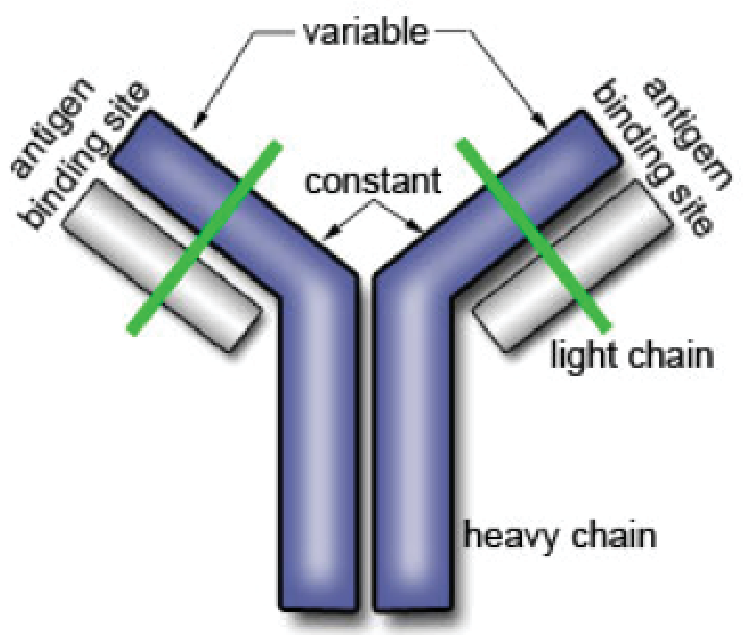
\includegraphics[width=.45\textwidth]{images/intro/figure1_1.pdf}
\caption[Overview of Antibody Structure]{
Overview of Antibody Structure. Heavy chain is shown in blue, light chain in grey. The structure is divided into the variable portion responsible for recognition, and the constant portion responsible for effector function. The apical tips of the antibodies are where antigens typically bind and are therefore known as the antigen binding sites. Image reproduced from http://crdd.osdd.net/raghava/absource/abasic.html.
}
\label{fig:antibodyoverview}
\end{figure}

\subsection{Antibody Diversification}
The antibody genes that encode heavy and light chains are located in three primary locations in the human genome: heavy chain genes (IGH) are located on chromosome 14, light chain kappa genes (IGK) are located on chromosome 2, and light chain lambda genes (IGK) are located on chromosome 22 \citep{Brochet:2008kq}. Each of these loci consists of multiple variable (V, not to be confused with the variable region of an antibody) and joining (J) gene segments. In addition the IGH locus also contains several diversity (D) gene segments.  Sequencing of the human IGH locus revealed 55 functional V genes, 23 D genes, and six J genes \citep{Matsuda:1998ua,Lefranc:2009ga}. The human variable genes (and, at the IGH locus, the diversity genes) can be phylogenetically grouped into families based on sequence similarity. Heavy chain variable genes are organized into seven families and homology within gene families is typically above 80\%. The 23 functional human diversity genes are also organized into seven families. An example variable gene, IGVH5-15*01, the standard IMGT nomenclature for human V and D genes follows the following pattern: the chain and gene description (IGHV for variable genes, IGHD for germline genes), the family, the gene number (determined by position in the germline locus), and the allele. The gene number is separated from the family with a hyphen and the allele is separated from the gene number with an asterisk.


\subsubsection{Recombination to Enable Diversity}
The tremendous sequence and structural diversity  can be attributed to two immunologic processes that act on antibody germline gene segments. The first is the initial recombination initiated by the recombination activating gene machinery (RAG) \citep{Brack:1978ie,Alt:1982uq,Tonegawa:1983vw,Schatz:1989tk,Oettinger:1990ud}. The RAG machinery is responsible for the recombination of V, D, and J gene for the heavy chain, and the V and J gene for the light chain (figure \ref{fig:Diversification}, left-panel). This process takes place to make functional B-cell receptors in the bone marrow before antigenic stimuli. If a B-cell receptor is found to bind self-antigens of the host, it is eliminated. This clonal selection and deletion is the fundamental process for which antibodies are able to recognize foreign antigens while not attacking the host.
 
Much progress has been made in determining the genetic and mechanistic elements that participate in the antibody recombination process. Recombination signal sequences (RSS), which flank V, D and J genes and are composed of conserved AT-rich heptamer and nonamer sequences separated by spacers of either 12 or 23 nucleotides, are recognized and bound by recombination activating gene (RAG1 and RAG2) proteins at the initiation of the recombination process \citep{Hesse:1989us,Alt:1992bh}. Recombination typically occurs only between RSS elements of different spacer lengths, in a model commonly referred to as the 12/23 rule of recombination \citep{Ramsden:1996tw,Steen:1996ut,vanGent:1996uw,Schatz:2011hb}. After binding to one 12-bp RSS and one 23-bp RSS, the RAG complex induces single-strand DNA nicks between the coding sequence and the heptamer of each RSS, resulting in hairpin formation on each of the coding ends and a blunt double-stranded break on each signal end \citep{Roth:1992wg,Schlissel:1993tg,McBlane:1995kp,Sadofsky:2001we}. The hairpins are opened with other RAG mutation machinery (Artemis) \citep{Ma:2002en}.  Nucleotides may be added to or removed from the coding ends, and the double strand breaks at the coding ends are joined into a single coding strand with DNA ligase IV \citep{Lewis:1994vp,Mahajan:1999wz,Shockett:1999vp,Walker:2001kn,MansillaSoto:2003ws,Roth:2003ji} (figure \ref{fig:Diversification}, middle panel). The newly recombined gene produces a functional antibody (figure /ref{fig:Diversification}, right panel). Recombination of the light chain is similar but the result of a single V$_{L}$J$_{L}$ recombination. To establish a diverse na�ve antibody repertoire, these events of RAG-mediated recombination produce an initial repertoire of ~3x10$^{7}$ different recombinations. This happens all before antigen stimulus in the bone marrow leading to the next form of antibody diversity, somatic hypermutation.

\begin{figure}%Recombination Diversification
\centering
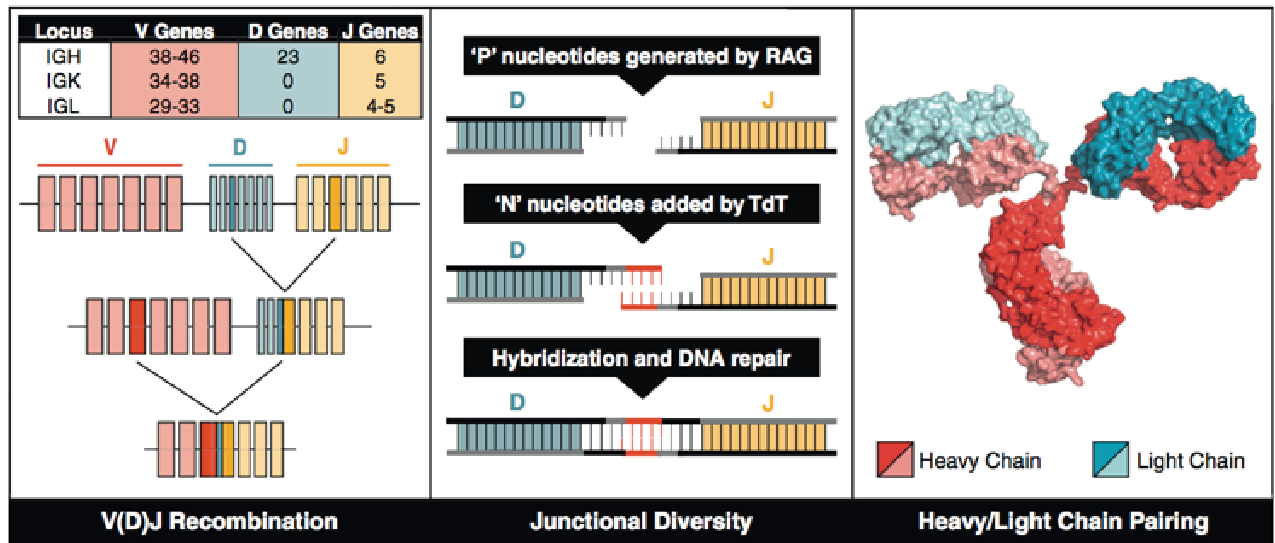
\includegraphics[width=1\textwidth]{images/intro/figure1_2.pdf}
\caption[Overview of Antibody Recombination]{
Overview of Antibody Recombination. Diversity in the antigen-combining site of the B-cell receptor repertoire (and thus also in the corresponding secreted antibody repertoire) is mediated by three principal molecular mechanisms, illustrated in the three panels, left, middle, and right. Figure adapted from \citep{Finn:2013fr}.
}
\label{fig:Diversification}
\end{figure}


\subsubsection{Somatic Hypermutation to Enable Diversity}
Maturation of the antibody repertoire to hone specificity is known as somatic hypermutation (SHM) and is initiated by the somatic hypermutation machinery (SHAM). Somatic hypermutation is the response to antigen stimulus and happens in various lymph tissues. This process is known as the secondary diversification \citep{Tonegawa:1983vw,Brenner:1966vj}. 

Na�ve, antigen inexperienced B-cells undergo the SHM process upon recognition of an infectious agent. It is through the SHM process, which occurs primarily in lymphoid tissue, mutate the variable region of their antibody genes (figure \ref{fig:somaticdiversification})  \citep{Li:2004it,MacLennan:1992we}. Many of these mutations have no effect on antigen recognition and many have deleterious effects on either antigen recognition or proper folding of the antibody protein. However, some mutations produce antibodies with improved affinity for the target pathogenic epitope  \citep{Casali:2006dn}.Thus, the SHM process provides a basis for the positive selection of high affinity antibodies that are characteristic of a mature immune response  \citep{MacLennan:1994bo}. SHM introduces point mutations at a frequency of approximately 103 mutations per base pair, which is 106-fold higher than the rate of spontaneous mutation in other genes \citep{Rajewsky:1987wn}. Activation-induced cytidine deaminase (AID) is required for SHM and initiates the SHM process by the deamination of cytosine nucleotides, which results in the conversion of cytosine to uracil \citep{Muramatsu:2000um,Muramatsu:1999ur}. Deamination thus produces a uracil-guanine mismatch, and several possible processes result in the error-prone repair of the mismatch. The precise mechanism(s) responsible for error-prone repair during SHM are not known, although several DNA repair mechanisms have been shown to be critical to the SHM process, including base excision repair and mismatch repair \citep{Phung:1998vx,Rada:1998tf,Wiesendanger:2000wl,DiNoia:2002ix,Zheng:2005dy}. 

\begin{figure}%Somatic Diversification
\centering
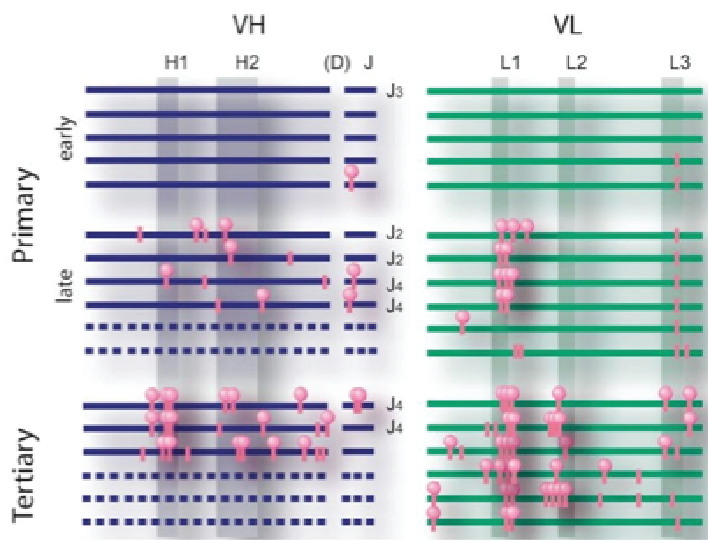
\includegraphics[width=.5\textwidth]{images/intro/figure1_3.pdf}
\caption[Somatic Mutations in Response to Antigen Stimulus]{
Somatic mutations in response to antigen stimulus. The VH gene and VL gene are shown for various VH and VL pairs represented by blue and green lines. The CDR loops H1-H3 and L1-L3 are darkened. The pink dots represent mutations. The early response has little to no somatic mutations recapitulating na�ve repertoire. The late and response starts developing mutations. A second challenge with the same antigen shows even more mutations to hone specificity. Figure adapted from \citep{Berek:1988ww}, redrawn by C., Scotti }
\label{fig:somaticdiversification}
\end{figure}

\subsubsection{Implications for Antibody Structure}
Antibody complementarity determining regions (CDRs, also referred to as hypervariable regions, figure /ref{fig:abwithloops}) are the primary region of antigen recognition that lie at the apical tip of the antibody structure (figure \ref{fig:abwithloops}). They are preferentially targeted for affinity maturation by the SHM machinery, making them the most variable regions of the antibody gene \citep{Padlan:1994wq}.  Structurally, the CDRs are largely loop-based, which make them sufficiently flexible to incorporate the substitutions and without compromising structural integrity. Framework regions (FRs) are highly structured and less able to accommodate somatic mutations \citep{Jimenez:2003by}.

\begin{figure}%Antibody with Loops
\centering
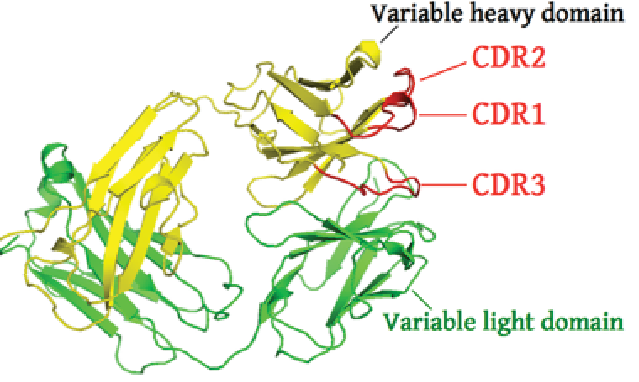
\includegraphics[width=.5\textwidth]{images/intro/figure1_4.pdf}
\caption[Antibody Structure with CDR Loops]{Antibody structure with CDRs.The light chain in green with the LCDRs not pictured. The heavy chain is shown in yellow with the HCDRs shown in red. Figure adapted from PDB: 1IGT\citep{Harris:1997eo}.
}
\label{fig:abwithloops}
\end{figure}

\section{HIV Pandemic Overview}
HIV-1 is an unprecedented health problem that continues to remain a worldwide pandemic. Since the recognition of acquired immune deficiency syndrome (AIDS) in 1981 \citep{Gottlieb:1981ge} followed by the discovery of it's causative agent, human immunodeficiency virus (HIV) in 1983 \citep{BarreSinoussi:1983ta}, an estimated 65 million have been infected with over 25 million deaths \citep{Hemelaar:2012cv}. The amount of people estimated to be still living with HIV is 30 million, many of which live in the developing world \citep{Anonymous:1vVbBZBX}.

More than 40 different nonhuman primate species harbor SIV infections, with each species carrying a species-specific virus. Each independent zoonotic transmission can generate a different lineage. HIV type 1 (HIV-1), thought to be transmitted from chimpanzees in the Congo around 1900 \citep{Keele:2006fi}, is the most common and further is split into groups M, N, O, and P. HIV-1 group M is responsible for the global pandemic and is further split into subtypes clades A-D,F-H, J and K that are tropic to specific regions. Within each subtype variation of the amino acids vary as much as 30\%. For example, clade B is the most common in North America while clade C is the most common in Sub-Saharan Africa (figure \ref{fig:pandemic}). If a full genome sequence is found that are recombinations of different HIV-1 group M subtypes, they are designated circulating recombinant forms (CRFs) if they are epidemiologically linked or unique recombinant forms if they are unlinked (URF) \citep{Robertson:2000bv}.

A major contributing factor to HIV spread and defense is its potential for enormous genetic diversity. This genetic diversity stems from the error rates of the reverse-transcription machinery which lacks proof-reading capabilities \citep{Ho:1995fn}. This genetic diversity gives rise to sequence divergence of up to 10\% within a single individual \citep{Korber:2001tc}. This is one of the many defense mechanisms HIV uses to evade host response and contemporary vaccination strategies.

\begin{figure}%HIV Pandemic
\centering
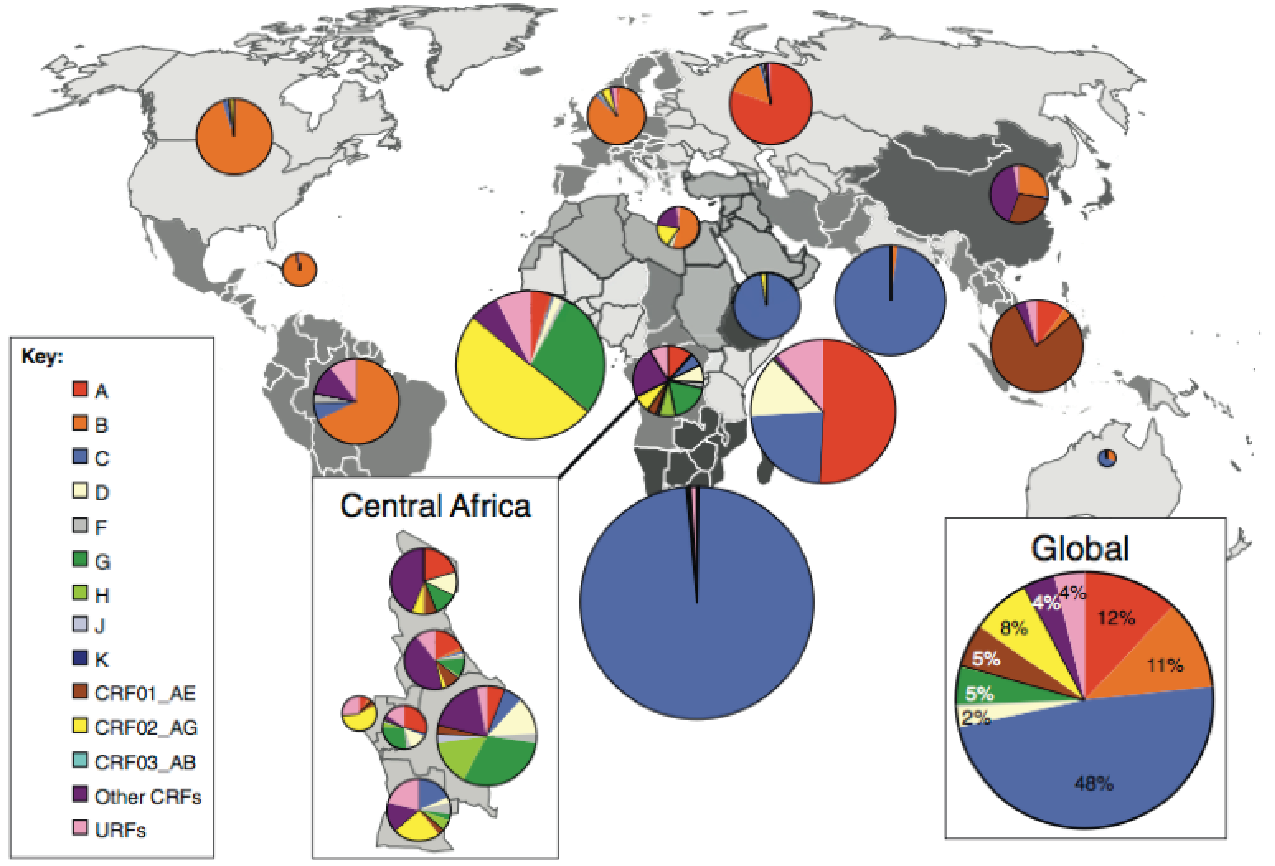
\includegraphics[width=1\textwidth]{images/intro/figure1_5.pdf}
\caption[Global Distributions of HIV-1 Subtypes]{Global distributions of HIV-1 subtypes. In the main figure, pie charts representing the distribution of HIV-1 subtypes and recombinants from 2004 to 2007, colored by HIV-1 subtype. Adapted from UNAIDS report 2013.}.
\label{fig:pandemic}
\end{figure}

\subsection{The HIV Virus Genome and Structure}
HIV-1 is an enveloped virus containing a duplicate positive-strand RNA genome (figure \ref{fig:hivgenome}, left panel). The functional spike on the surface of the virion is the Env glycoprotein and is coded by the env gene (figure \ref{fig:hivgenome}, right panel). The Env glycoprotein complex is originally produced as a single-chain glycoprotein precursor, gp160, which is cleaved by a cellular protease. Cleavage of gp160 results in the cell-surface attachment protein gp120 and the membrane-spanning protein gp41. The gp160 cleavage products are noncovalently linked and assemble into a trimer of gp120-gp41 heterodimers that are expressed on the virion surface \citep{Kowalski:1987vq}. Gp120 is heavily glycosylated, with nearly half the total mass being the result of N-linked glycans \citep{Poignard:2001hu}. It is composed of five variable regions (V1-V5) interspersed with five constant regions (C1-C5) \citep{Starcich:1986ty}. The principle function of the glycoprotein spike is to facilitate cell entry by binding to the primary cell-surface receptor, CD4, and one of the two co-receptors, CCR5 and CXCR4. Binding to the receptor and co-receptor is accomplished by gp120, and fusion of the viral and cell membranes is mediated by gp41 \citep{Zwick:2001ei}. 

The rest of the genome is composed of viral enzymes such as the error-prone reverse transcriptase, the integrase that allows integration of viral DNA to the host genome, and protease, to allow cleavage of gene products into their functional subunits. There are also structural proteins that lie below the envelope that make up the inner matrix and nucleocapsid. There are also several accessory proteins, Vpu, Vif, Vpr, P6, Nef, Rev, and Tat which aid in combating host defense or enhancing viral fitness \citep{Fields:2007vu}. All of these proteins serve a significant purpose to the virulence and life cycle of the HIV-1 virus but will not be discussed further and they have low antigenicity to antibodies, the primary focus of my research. A list of their genes and gene products can be found in figure \ref{fig:hivgenome}, right panel. 

\begin{figure}%HIV Genome and Structure
\centering
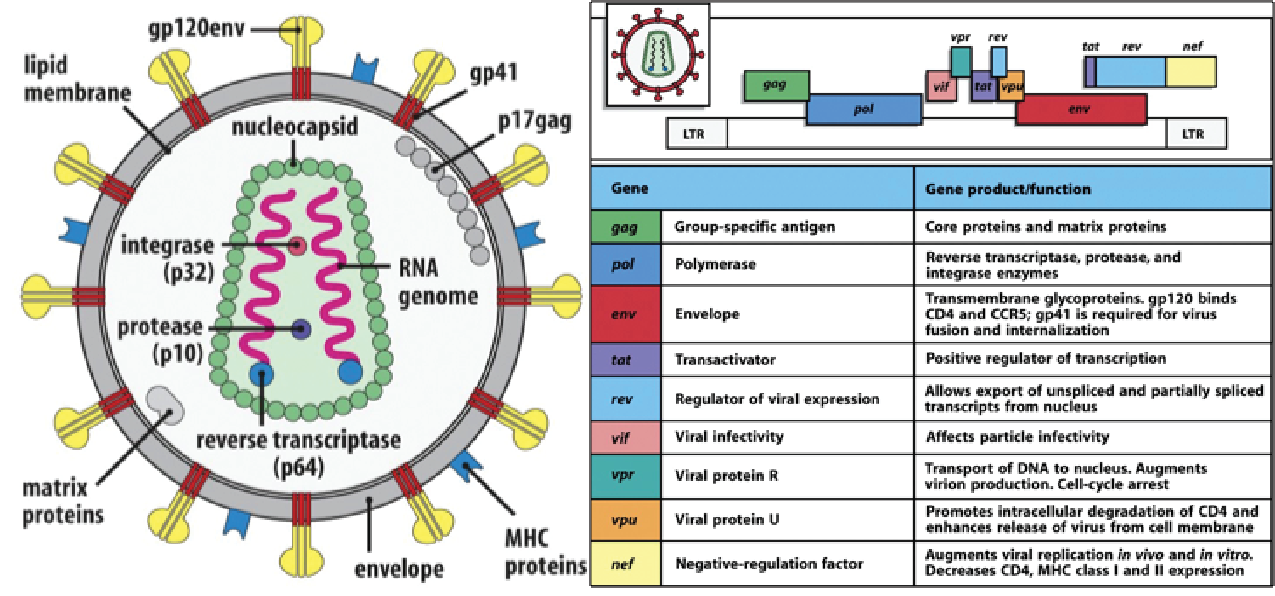
\includegraphics[width=1\textwidth]{images/intro/figure1_6.pdf}
\caption[Simplified View of HIV Structure and Genome]{Simplified view of HIV structure and genome. The proteins that make up the virus structure are displayed as a schematic. The virus is coded by a duplicated RNA genome (pink) surrounding by a viral nucleocapsid proteins. The inner envelope is supported by gag protein with gp120 envelope shown as a trimer bound to gp41. These trimeric "spikes" are responsible for infectivity by binding CD4-binding sites (left panel).\linebreak Each gene is represented in a different color and localizes to either the nucleocapsid (green) or the outer envelope (red). }
\label{fig:hivgenome}
\end{figure}

\subsection{The Viral Spike and Humoral Resistance}
The failure of conventional vaccines to prime the immune system for a broad response against HIV-1 challenge is partially explained thorough the structural definition of the HIV-1 spike reveling mechanisms of defense. Much of the surface is covered in carbohydrates that shield neutralizing epitopes \citep{Binley:2010du}. The conserved CD4 binding site is recessed and sits behind the hypervariable loops \citep{Burton:2005db}. The co-receptor binding site is also recessed unless CD4 has triggered a conformational shift exposing this region \citep{Harris:2011gm}. Another defense is the relative lability of the trimeric complex \citep{Wyatt:1998vs}. The gp120 head often sheds creating "stumps" that serve as decoy epitopes against the viral complex \citep{Liu:2008in}. In addition there are few functional trimeric spikes on the surface of HIV limiting immune response to few locations on the virion. 

The biggest defense is sequence variability. Much of the antibody response is targeted to the hypervariable loops that can easily change sequence without much consequence to viral fitness. This is why the humoral response produces autologous or strain-specific neutralizers that must catch up to a constantly evolving antigenic target \citep{Albert:1990ua,Gray:2007hi,Pilgrim:1997wj,Richman:2003dc,Sagar:2006eb,Wei:2003ea}.  

\section{Broadly Neutralizing Antibodies to HIV}
Given the major defenses of the HIV envelope structure, it provided a rather discouraging view for vaccine development. In fact, only four modestly neutralizing antibodies were discovered between the 1991 and 2010 \citep{Burton:2005db,Kwong:2012cc}, two membrane proximal extracellular region (MPER) binders 2F5 and 4E10 \citep{Zwick:2001ei,Muster:1994tw}, a CD4 binding site neutralizer b12 \citep{Burton:1994wl}, a complex carbohydrate binder 2G12 \citep{Trkola:1996vb} (table \ref{tab:allmabs}, figure \ref{fig:bnabmap}). 

It was thought that the conventional vaccine strategies could not stimulate immune system to produce broadly neutralizing antibodies to HIV do to the extreme variability of the viruses and the capability of the virus to escape an antibody response. Then, high throughput neutralization assays were developed that could rapidly test sera for neutralization capacity \textit{in vitro} allowing researchers to accurately quantify the neutralizing response of HIV infected patients \citep{Binley:2004hd,Blish:2007ef,Li:2005go,Mascola:2005fe,Montefiori:2005jt}. Several groups found that there were multiple patients that could neutralize very genetically diverse panels HIV variants, even those that were not in that patients sub-type \citep{Binley:2008gj,DoriaRose:2010js,Simek:2009cn,Wu:2006cd}. That lead to longitudinal studies to show how long it took for a broadly neutralizing response to develop. Researchers showed that this generally took anywhere from 2-4 years \citep{Gray:2011ki,Mikell:2011hr,Moore:2011hy} with earliest time points arising at 1 year \citep{DoriaRose:2014ic}. The question still remained if those neutralizing responses were caused by few monoclonal antibody responses or just a large polyclonal response \citep{Gray:2007hi,Binley:2008gj,Li:2007em,Rong:2009ky,Sather:2009jb,Scheid:2009bv,Tomaras:2011bc,Walker:2010bm}.

The question was answered by the recent explosion of new broadly neutralizing antibodies isolated by multiple research groups \citep{Corti:2013ex}. It started with two new isolates, PG9 and PG16, from an African donor that lead to the discovery of a completely new neutralizing epitope which is the focus of my research (figure  \ref{fig:bnabmap}) \citep{Walker:2009cd}. Both PG9 and PG16 bind to a proteoglycan epitope through an extended HCDR3 structure \citep{McLellan:2011dg}. 

The discovery of PG9 and PG16 lead to newly characterized antibodies using similar techniques such as microneutralization screening, high-throughput sequencing, and hybridoma technology. The Haynes laboratory characterized additional long HCDR3 antibodies that bound similarly as PG9 and PG16 but with less breadth \citep{Bonsignori:2011dq}. There are other classes of glycan dependent antibodies isolated by the Poignard group that bind the V3 and beta-strands that are higher potency than PG9 and PG16 \citep{Walker:2011ew}. Other MPER antibodies have also been characterized to by the Connors group such as 1E08 that neutralizes 98\% of viruses \citep{Huang:2012fh}. Focused epitopes designed computationally can also be used to identity some of the most potent antibodies to date (the VRC series) \citep{Wu:2010jv}. These antibodies were identified using a designed scaffold of gp120 that 'knocked-out' non-neutralizing epitopes. Thus, only neutralizing antibodies would be isolated upon binding. I will not enumerate further on all the antibodies characterized to date, their method of isolation and if any longitudinal studies were used to determine their pathways of development. These characteristics are summed in table \ref{tab:allmabs} and figure \ref{fig:bnabmap}.

It is interesting to note, and important for the work that will be presented here, that the broadly neutralizing antibodies to date share one of two characteristics. They are either highly somatically mutated, indicative of years of chronic infection and selective pressure, or have a very long non-canonical HCDR3 (figure \ref{fig:bnabcorrelabion}). Both of these characteristics make it difficult to elicit in a vaccine attempt, but will be discussed further in the upcoming chapters.

%comes from excel to table
% Table generated by Excel2LaTeX from sheet 'page 1'
\begin{sidewaystable}[htbp]
  \centering
\begin{tabular}{lllllcl}
\toprule
Antibody & Specificity & Breadth & V$_{H}$ & SHM & HCDR3 Length & Screening Strategy \\ 
\midrule
	2F5 & gp41 MPER & \textasciitilde60-70\% & 2-5 & 15.2 & 24 & gp160 and p24 binding \\
	4E10 & gp41 MPER & \textasciitilde96-98\% & 1-69 & 15.6 & 20 & gp160 and p24 binding   \\ 
	1EO8 & gp41 MPER & \textasciitilde98\% & 3-15 & 22.1 & 22 & Microneutralization  \\ 
	2G12 & gp120 glycans & \textasciitilde25-30\% & 3-21 & 33.6 & 16 & gp160 and p24 binding   \\ 
	PGT128 & Glycans and V3 $\beta$-strand & \textasciitilde70-75\% & 4-39 & 27.9 & 21 & Microneutralization  \\ 
	PGT127 & Glycans and V3 $\beta$-strand & \textasciitilde50\% & 4-39 & 23.2 & 21 & Microneutralization   \\ 
	PGT121 & Complex type V3 N-glycans & \textasciitilde65-70\% & 4-59 & 21.2 & 26 & Microneutralization  \\ 
	10-1074 & Complex type V3 N-glycans & \textasciitilde55-60\% & 4-59 & 24.4 & 26 & gp140 binding   \\ 
	PGT135 & Glycans and V4 & \textasciitilde30-35\% & 4-39 & 26.8 & 20 & Microneutralization   \\ 
	PG9/PG16 & Glycans and V1/V2 & \textasciitilde75-80\% & 3-33 & 15.4-16.8 & 30 & Microneutralization   \\ 
	CH01- CH04 & Glycans and V1/V2 & \textasciitilde50\% & 3-20 & 23.3-19.5 & 26 & Microneutralization  \\
	PGT145 & Glycans and V1/V2 & \textasciitilde75-80\% & 1-8 & 22.8 & 33 & Microneutralization \\
	b12 & gp120 CD4bs & \textasciitilde30-35\% & 1-3 & 17.3 & 20 & Phage library  \\ 
	HJ16 & gp120 CD4bs & \textasciitilde30-35\% & 3-30 & 36.7 & 21 & EBV- immortalization  \\ 
	VRC01 & gp120 CD4bs & \textasciitilde90-95\% & 1-2 & 38.7 & 14 & Cell sorting/RT-PCR \\
	VRC03 & gp120 CD4bs & \textasciitilde50\% & 1-2 & 34.9 & 16 & Cell sorting/RT-PCR \\ 
	3BNC117 & gp120 CD4bs & \textasciitilde85-90\% & 1-2 & 36.9 & 12 & Cell sorting/RT-PCR  \\ 
	3BNC60 & gp120 CD4bs & NA & 1-2 & 36.9 & 12 & Cell sorting/RT-PCR \\
	NIH45-46 & gp120 CD4bs & \textasciitilde90\% & 1-2 & 44 & 18 & Cell sorting/RT-PCR \\
	CH30- CH34 & gp120 CD4bs & \textasciitilde80\% & 1-2 & 31.9-31.9 & 15 & Cell sorting/RT-PCR  \\
	PGV04 & gp120 CD4bs & \textasciitilde85-90\% & 1-2 & 38.2 & 16 & Cell sorting/RT-PCR\\
	3BC176 & CD4i/V3 & \textasciitilde60-70\% & 1-2 & 29.4 & 19 & Cell sorting/RT-PCR \\
\bottomrule
\end{tabular}
\caption[Broadly Neutralizing Antibody Properties]{Broadly neutralizing antibody properties. Breadth refers to the amount of viruses tested that fall below 50 $\mu$g/mL.  V$_{H}$ is the heavy chain accessed from IMGT, SHM is the somatic hypermutation percentage of heavy chains as assessed from IMGT. Table adapted from (2013)\citep{Corti:2013ex}. }
\label{tab:allmabs}%
\end{sidewaystable}%


\begin{figure}%HIV man map
\centering
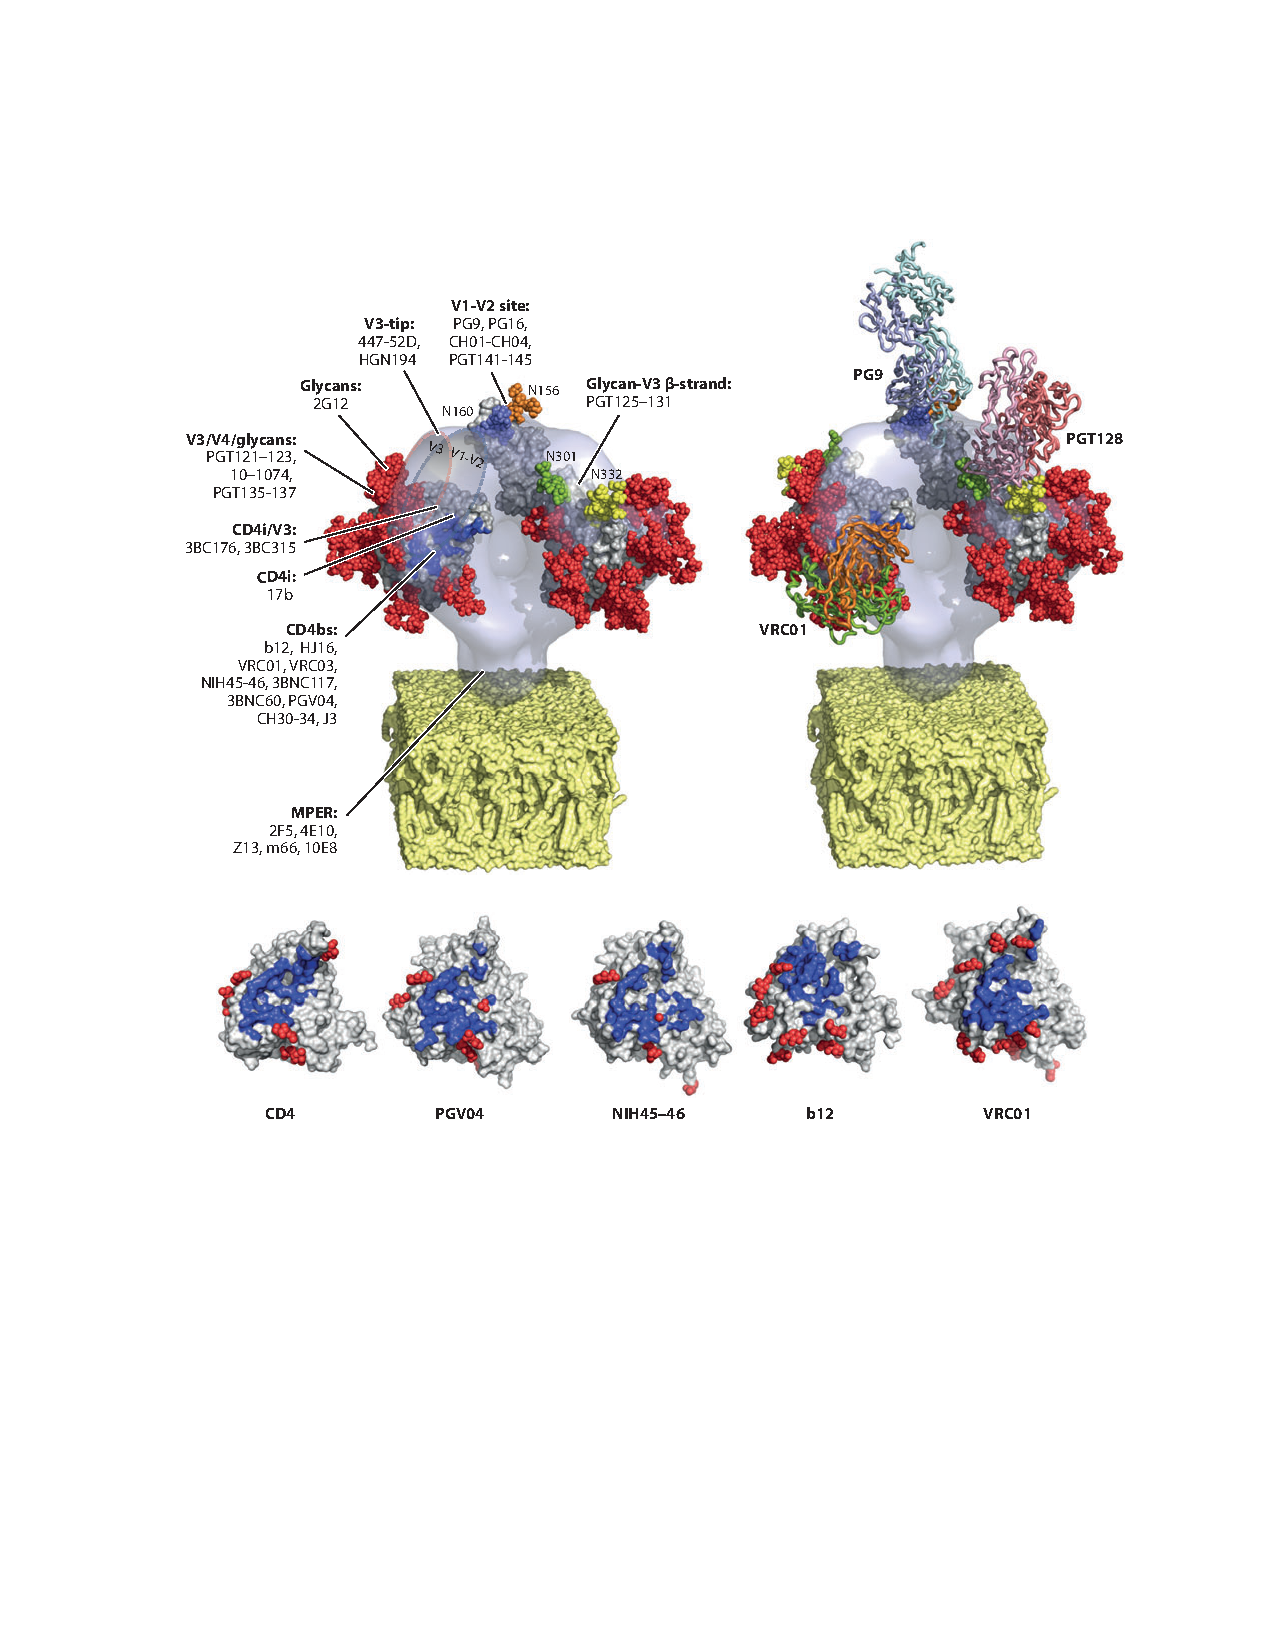
\includegraphics[width=1\textwidth]{images/intro/figure1_7.pdf}
\caption[Broadly Neutralizing Epitopes Mapped to HIV Env Trimer]{Model of the HIV-1 Env trimeric glycoprotein bound to broadly neutralizing antibodies. The left panel shows the major sites targeted by broadly neutralizing antibodies. The approximate positioning of the V1/V2 and V3 loops is shown, and the CD4 footprint on the gp120 monomer is highlighted in blue. The right panel shows the FABs of broadly neutralizing antibodies VRC01 (3NGB), PG9 (3US2), and PGT128 (3TYG) bound to gp120. Carbohydrates (oligomannose, red spheres) were modeled on the unliganded YU2 gp120 core (3TGQ) using GlyProt, with the exception of the glycans bound by PGT128 and PG9 (depicted with different colors), which were taken from the structures. The location of PG9 above the trimeric gp120 is approximate; VRC01 and PGT128 FABS were docked by superposition with the unliganded YU2 gp120 model. The bottom panel shows in blue the footprints of CD4 (1GC1) and the CD4bs-specific antibodies PGV04 (3SE9), NIH45-46 (3U7Y), b12 (3DNL), and VRC01 (3NGB). Figure adapted from \citep{Corti:2013ex}}
\label{fig:bnabmap}
\end{figure}

\begin{figure}%HIV man map
\centering
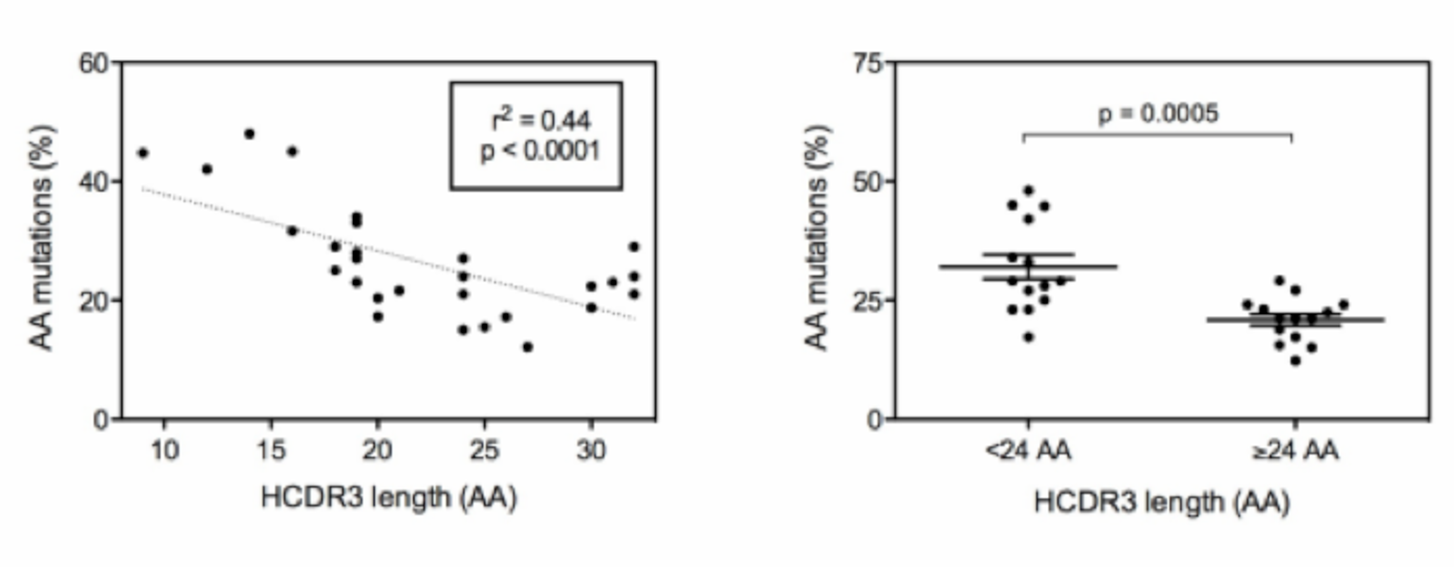
\includegraphics[width=1\textwidth]{images/intro/figure1_8.pdf}
\caption[Trends of HIV bNAbs]{Trends of HIV bNAbs. Plotted on the y-axis is the frequency of amino acid mutations of the currently characterized bNAbs. On the x-axis is the length of the heavy chain CDR3 (HCDR3). A negative correlation exists between the frequency of mutations and the HCDR3 length (r$^{2}$ = 0.44, left panel). When long HCDR3s (>24 AA) are binned against canonical length HCDR3s (<24AA), there is a statistical significance between the frequencies of amino acid mutation (p = 0.0005, right panel).}
\label{fig:bnabcorrelation}
\end{figure}



\section{Rosetta}
Many software packages exist for the specific task of threading, minimization, and design. The Rosetta software suite includes algorithms for all of these tasks and was developed for computational modeling and analysis of protein structures; further, it is free for noncommercial users. It has enabled notable scientific advances in computational biology, including de novo protein design, enzyme design, ligand docking and structure prediction of biological macromolecules and macromolecular complexes \citep{Rohl:2004bl,Siegel:2010bc,Kuhlman:2003kp,Davis:2009bf,Misura:2006hs,Davis:2009fx,Das:2008gf}. The broad spectrum of applications available through Rosetta allows for multiple computational problems to be addressed in one software framework. To aid in the understanding of Rosetta-specific language, a supplementary glossary has been provided in the appendix section for the Rosetta glossary.
One of the most common applications of Rosetta is protein structure prediction via \textit{de novo} folding and comparative modeling \citep{Kaufmann:2010ea,Rohl:2004bl}. \textit{De novo} folding can be used to predict the protein's tertiary structure when only the primary sequence of a protein is known. However, to date, Rosetta has been shown to successfully fold only small, soluble proteins (fewer than 150 amino acids), and it performs best if the proteins are mainly composed of secondary structural elements \citep{Meiler:2003dt}. Structures of helical membrane proteins between 51 and 145 residues were predicted to within 4� of the native structure \citep{YarovYarovoy:2006br}, but only very small proteins (up to 80 residues) have been predicted to atomic-detail accuracy \citep{Bradley:2005bu,Bradley:2005fs,Das:2007em}. Accurate prediction of larger and/or more complex proteins can be achieved with the addition of experimental data, such as NMR chemical shifts and distance data \citep{Rohl:2005kx,Lange:2012hp,Lange:2012wo}.

Another application, protein threading, refers to the tolerance of a tertiary fold given PDB coordinates. The Rosetta scoring function evaluates how well a sequence can "tolerate" a structure. It is often known as the "inverse folding problem". The known template structure of which a sequence will be threaded reduces almost all-conformational space by providing a protein backbone scaffold. Threading has played a major role in aiding experimental design and the interpretation of experimental results. They can be used to help predict structure-function relationships \citep{Kaufmann:2009cq}, and aiding in designing proteins for binding pathogens \citep{Azoitei:2011jd,Correia:2010ck,Correia:2011bk,Correia:2011hr,Schief:2009ke}, determining thermostable proteins \citep{Stranges:2013em,Kuhlman:2002ka,Der:2011gt},and aid in the determination of target residues for site-directed mutagenesis \citep{Keeble:2008hd,Fortenberry:2011gx}. 

\subsection{The Rosetta Energy Function}
All of the applications described above rely on a metric to score predictive models. This metric in Rosetta is referred to as the Rosetta energy function. The scoring function in Rosetta is derived empirically through analysis of observed geometries of a subset of proteins in the PDB. We call this scoring function a knowledge-based scoring function, since it relies on previous knowledge of observed structures. The measurements include, but are not limited to, radius of gyration, packing density, distance/angle between hydrogen bonds and distance between two polar atoms. The measurements are converted into an energy function through Bayesian statistics \citep{Simons:1997do,Metropolis:1953vj}.

The scoring function in Rosetta can be separated into two main categories: centroid-based scoring and all-atom scoring. The former is used for de novo folding and initial rounds of loop building \citep{Rohl:2005kx,Simons:1997do,Simons:1999wp}. The side chains are represented as "super-atoms", or "centroids", which limit the degrees of freedom to be sampled while preserving some of the chemical and physical properties of the side chain. Although this centroid-based scoring function is important for de novo folding, the folding protocol is not covered within the scope of this article.

The all-atom scoring function represents side chains in atomic detail. Similarly to the centroid-based scoring function, the all-atom scoring function comprises weighted individual terms that are summed to create a total energy for a protein. Most of the scoring terms are derived from knowledge-based potentials. The scoring function contains Newtonian physics based terms, including a 6-12 Lennard-Jones potential and a solvation potential. The 6-12 Lennard-Jones potential is split into two terms, an attractive term (fa\_atr) and a repulsive term (fa\_rep), for all van der Waals interactions \citep{Kuhlman:2000tc,Neria:1996wj}. The solvation potential (fa\_sol) models water implicitly and penalizes the burial of polar atoms \citep{Lazaridis:1999wi}. Interatomic electrostatic interactions are captured through a pair potential (fa\_pair) \citep{Simons:1999wp}, and an orientation-dependent hydrogen bond potential for long-range and short-range hydrogen bonding (hbond\_sc, hbond\_lr\_bb, hbond\_sr\_bb, and hbond\_bb\_sc, respectively) \citep{Gordon:1999tk,Wedemeyer:2003kh}. In addition to the electrostatic terms, the Rosetta all-atom scoring function contains terms that dictate side chain conformations according to the Dunbrack rotamer library (fa\_dun) \citep{Dunbrack:1993jt,Dunbrack:1997kh}, preference for a specific amino acid given a pair of phi/psi angles (p\_aa\_pp), and preference for the phi/psi angles in a Ramachandran plot (rama) \citep{Rohl:2004bl,Wedemeyer:2003kh,RAMACHANDRAN:1963wj}.

\subsection{Rosetta Minimization}
\label{subsec:Rosetta Minimization}
When new sequences are threaded, or rebuilt onto target protein structures, it is often necessary to go through a round of energetic minimization. The protein undergoes refinement using the Rosetta all-atom scoring function to yield an all-atom protein model \citep{Bradley:2005bu}. Both threading and docking in Rosetta involve an all-atom refinement of the protein. The protocol used for structural refinement, visually described in figure \ref{fig:minimization}, is often referred to as "relax". The goal of the relax protocol is to explore the local conformational space and to energetically minimize the protein. During this process, local interactions are improved by iterative side-chain repacking, in which new side chain conformations, or "rotamers", are selected from the Dunbrack library \citep{Dunbrack:1993jt}; and by gradient-based minimization of the entire model, in which the energy of the model is minimized as a function of the score. These small structural changes are evaluated according to the all-atom scoring function and are sampled in a Metropolis Monte Carlo method \citep{Metropolis:1953vj}. The relax protocol has been shown to markedly lower the overall energy of the Rosetta model and is essential to achieving atomic detail accuracy \citep{Das:2008gf,Bradley:2005fs,Rohl:2005kx}.

\begin{figure}%minimization
\centering
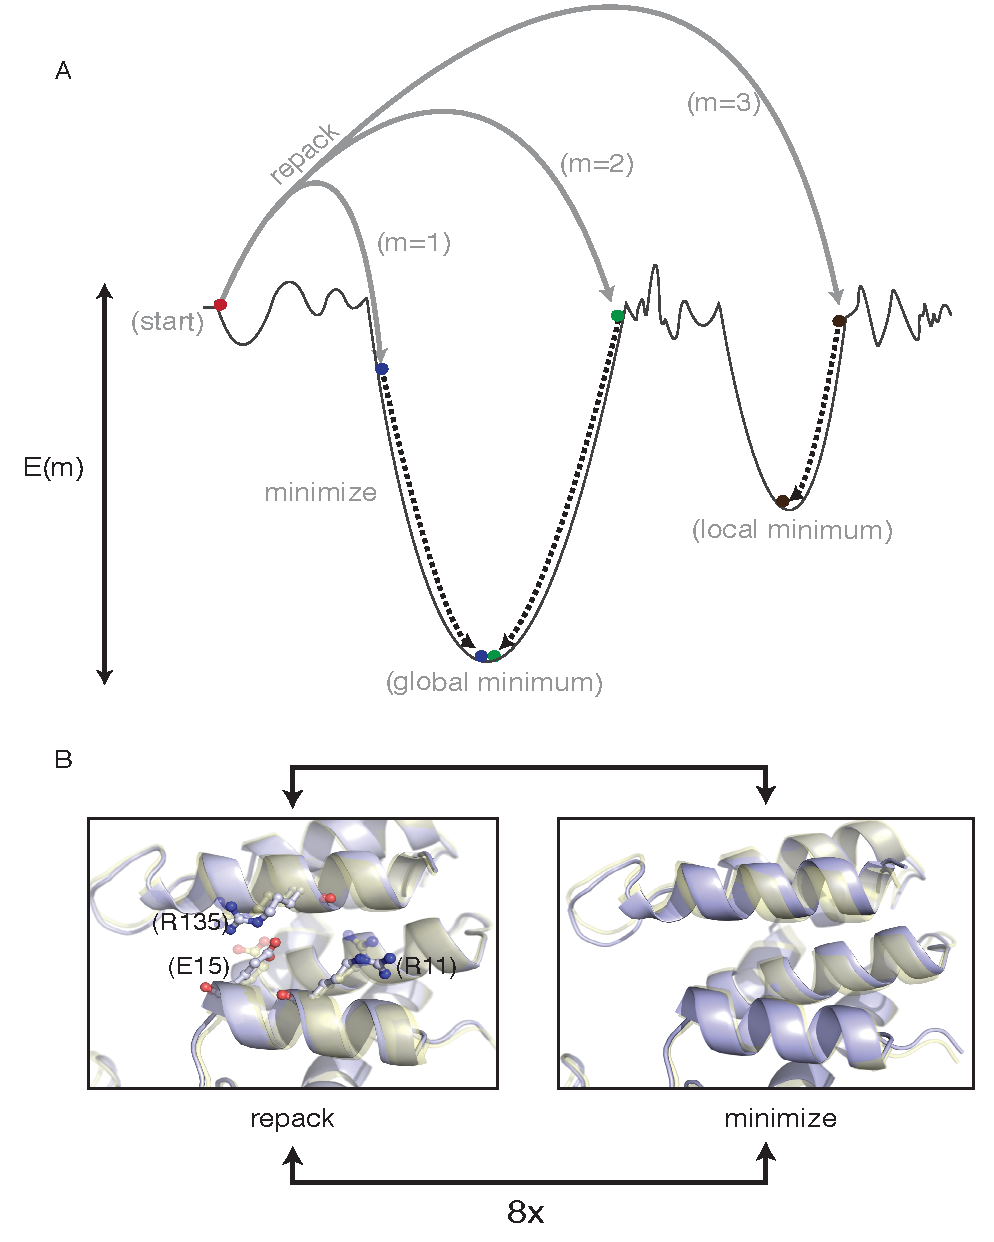
\includegraphics[scale=.7]{images/intro/figure1_9.pdf}
\caption[Refinement via Relax]{Refinement via Relax. Simplified energy landscape of a protein structure. The relax protocol combines small backbone perturbations with side-chain repacking. The coupling of Monte Carlo sampling with the Metropolis selection criterion allows for sampling of diverse conformations on the energy landscape. The final step is a gradient-based minimization of all torsion angles to move the model into the closest local energy minimum (A). Comparison of structural perturbations introduced by the repack and minimization steps. During repacking, the backbone of the input models fixed, whereas side-chain conformations from the rotamer library33 are sampled. Comparison of the initial (transparent yellow) and final (light blue) models reveals conservation of the R135 rotamer but changes to the R11 and E15 rotamers. Minimization affects all angles and changes the backbone conformation (B).}
\label{fig:minimization}
\end{figure}



\subsection{Rosetta Design}
Protein design, seeks to determine an amino acid sequence that folds into a given protein structure or performs a given function. The RosettaDesign algorithm is an iterative process that energetically optimizes both the structure and sequence of a protein \citep{Kuhlman:2003kp}. RosettaDesign alternates between rounds of fixed backbone sequence optimization and flexible backbone energy minimization. During the sequence optimization step, a Monte Carlo simulated annealing search is used to sample the sequence space. Every amino acid is considered at each position in the sequence, and rotamers are picked from to the Dunbrack library \citep{Dunbrack:1993jt}. After each round of Monte Carlo sequence optimization, the backbone is relaxed to accommodate the designed amino acids. The practical uses of RosettaDesign can be divided into five basic categories: design of novel folds. Redesign of existing proteins, design to enhance knowledge of structure, enzyme design, and design applied to translational medicine. 

\subsubsection{Design of Novel Folds}
The RosettaDesign method was implemented by Kuhlman and colleagues \citep{Kuhlman:2000tc}. The method has been used for the \textit{de novo} design of a fold that was not (yet) represented in the PDB \citep{Kuhlman:2003kp}. This was arguably the start of the "golden age" of protein design and gave credibility to the algorithm. A starting backbone model consisting of a five-strand $\beta$-sheet and two packed helices was constructed with the Rosetta \textit{de novo} protocol using distance constraints derived from a two-dimensional sketch. The sequence was iteratively designed with five simulation trials of 15 cycles each. The final sequence was expressed, and the structure was determined using X-ray crystallography. The experimental structure has a deviation to the predicted structure of <1.1 angstroms.

\subsubsection{Redesign of Existing Proteins}
When nine globular proteins were stripped of all side chains and then redesigned using RosettaDesign, the average sequence recovery was 35\% for all residues \citep{Dantas:2003vt}. In four of nine cases, the protein stability improved as measured by chemical denaturation. The structure of a redesigned human protein was determined experimentally.  RosettaDesign was then used to systematically identify mutations of carboxypeptidase that would improve the stability of the protein. All of the tested mutants were more stable than the wild-type protein, with the top-scoring mutant having a reduction of free energy of 5.2 kcal/mol.

\subsubsection{Design to Enhance Knowledge of Structure}
Protein design approaches have enhanced our knowledge of how protein sequence relates to protein structure. For instance, the finding that designed protein sequences are highly similar to the native sequence suggests that native protein sequences are optimal for their structure \citep{Kuhlman:2000tc}. Babor and Kortemme investigated the antibody sequence-structure relationship using RosettaDesign. They demonstrated that native sequences of antibody HCDR3 loops are optimal for conformational flexibility \citep{Babor:2009it}. The authors collected pairs of unbound and antigen-bound antibody structures. They used multiconstraint design to find low-scoring sequences that were consistent with both unbound and bound structures. The sequences predicted by multiconstraint design were more similar to the native sequences than the sequences predicted to preferentially bind either the unbound or bound conformations. 

\subsubsection{Enzyme Design}
The RosettaMatch algorithm starts from the protein backbone and attempts to build toward the specified transition state geometry \citep{Zanghellini:2006is}. In this method, all possible active site positions are defined for the protein scaffold, and rotamers from the Dunbrack library are placed at each sequence position in the catalytic site. The sequence of the area surrounding the catalytic site is then designed. 
Recently, the RosettaMatch algorithm was used to design enzymes that catalyze the retro-aldol reaction \citep{Jiang:2008jk}.The degrees of freedom in the transition state, the orientation of the active site side chains, and the conformations of the active site side chains were simultaneously optimized. Of 72 models tested, a total of 32 were found to have catalytic activity as much as four orders of magnitude greater than that of an uncatalyzed reaction. Two of the active enzymes were crystallized. The experimental structures share a high degree of similarity with the computational design although the loop regions surrounding the catalytic site show significant variance from the model.

Computationally designed functional Kemp elimination catalysts using RosettaMatch have also been designed. Quantum chemical predictions were used to generate an idealized transition state model, and RosettaMatch was used to search for backbone configurations that would support the predicted transition sate \citep{Rothlisberger:2008ef}. 

\subsubsection{Design Applied to Translational Medicine}
The successes of the RosettaDesign algorithm in predicting new sequences that optimize binding and answer questions about protein structure lead to its application to more bio-medical applications such as vaccine design and protein therapeutics. Fleishman et al. used the paratope of an antibody to find hotspot positions that neutralized influenza. Using these positions, they designed a protein that would properly present a mimic of the paratope. The crystal structure of the design indicated that it did indeed present mimicry while functional studies confirmed its neutralization capacity \citep{Fleishman:2011fx}.
The works of the Schief group have expanded design to explore novel scaffolding approaches to be used as immunogens. Using RosettaDesign, they presented the epitope to broadly neutralizing antibodies 2F5 and 4E10 to HIV which elicited this class of antibody in animal models \citep{Correia:2010ck,Ofek:2010bv}. In addition, they have used RosettaDesign to target potently neutralizing antibodies against the CD4 site while eliminated binding to non-neutralizing antibodies that bind to decoy epitopes \citep{Wu:2010jv}. More recently, this lab has used design to mimic an epitope to RSV that is now being tried in animal models \citep{Correia:2014jp}.

A current major challenge in protein design is the \textit{de novo} design of a novel protein-protein interface. So far, the most successful attempts at \textit{de novo} interface design have been relatively modest, focusing on small proteins and yielding micromolar affinity \citep{Mandell:2009he,Huang:2007ge}. This small boost affinity often requires display technology to increase potency and specificity. The Rosetta community is well aware of these limitations and work on increasing the accuracy of predicted interface mutations, particularly around hydrogen bonding networks and explicit solvent models \citep{Combs:2012tl}. 



\chapter{Mechanisms of Polyspecificity}
\label{chap:chapter2}
\section{Introduction}
Human antibodies are critical for eradication of viral and bacterial infections, while providing the basis for immunological memory. Antibody protein molecules are encoded by several recombined germline gene segments prior to antigen exposure. The initial set of antibodies that are generated by recombination in the bone marrow is the antigen-na�ve antibody repertoire. It is of great interest to know how a finite set of such germline gene-encoded antibodies can recognize the large number of possible foreign antigens. A current hypothesis in the field suggests that antibodies encoded by germline gene segments are structurally flexible and therefore able to accommodate binding to many antigens, much like one glove fitting the shape of many hands. The phenomenon of one structure binding to many unrelated targets is known as polyspecificity. In this chapter, I will describe how I further support this hypothesis using computational design by showing the entire antibody protein variable region sequence is close to ideal for polyspecificity by mechanisms of flexibility. I will detail the computational protocol I have developed and the results that suggest how a finite set of antibody germline gene segments can encode antibodies that can engage a large number of potential antigens. Computational design of antibodies capable of binding multiple antigens may allow the rational design of antibodies that retain polyspecificity for diverse epitope binding, which will be an important to future vaccine design.

\subsection{Three Models of Protein Binding}
Antibodies are encoded by the rearrangement of variable (V), diversity (D), and joining (J) gene segments into recombined genes that encode a large but ultimately finite number of unmutated antibody structures, known as the germline repertoire \citep{Tonegawa:1983vw}. There are approximately 10$^{4}$ combinations of the V, D, and J heavy chain gene segments and an estimated 10$^{11}$ possible combinations when junctional diversity is considered \citep{Patten:1996vm}. This number of potential antibodies is far less than the immeasurable number of epitopes on foreign antigens to which one could be exposed. The germline gene repertoire therefore encodes a finite number of starting structures in the germline repertoire that must be capable of recognizing and binding a large and diverse array of antigens \citep{Patten:1996vm,Schultz:2002ef,Collins:2003wv}.

The classical protein binding mechanism was the "lock-and-key" model, where antibodies acquired somatic mutations in order to rigidify a pre-bound structure that would complement the shape of the epitope (figure \ref{fig:abmechanism}A). This mechanism dominated the field for many years but has to assume that one antibody optimally binds to one particular antigen \citep{Notkins:2004iz,James:2003ts}. The lock-and-key model has many shortcomings, as the "one paratope-one epitope" principle leaves little room to describe the polyspecificity phenomenon, an antibody's ability to recognize multiple unrelated antigens.

Polyspecificity has been demonstrated in a variety of biochemical and structural studies, therefore the "lock-and-key" model cannot possibly describe all antibody-antigen interactions without the existence of multiple paratopes per antibody \citep{Schultz:2002ef,Yin:2003wb,James:2003ip,Foote:1994tr}. In contrast to the "lock-and-key" model, a degree of pre-bound structural flexibility are found in two models of antigen binding, the "induced-fit" and the "conformational flexibility" models. In these models, germline gene-coded antibodies retain a degree of structural plasticity in their backbone in order to bind a number of different unrelated antigens. The induced-fit model hypothesizes that upon binding conformational changes are induced to accommodate the interacting structure (figure \ref{fig:abmechanism}B) \citep{Notkins:2004iz,James:2003ip}.

The conformational flexibility hypothesis in protein binding suggests that an unbound protein assume a variety of conformations (conformational isomerism), a subset of which is recognized by the interacting partner (figure \ref{fig:abmechanism}C). For antibodies, a large body of work has attributed polyspecificity to the nature of their germline gene sequences. It has been reported that polyspecific antibodies often retain a larger proportion of germline gene sequences than more mature, specific antibodies \citep{Notkins:2004iz,Chen:1991ug,Crouzier:1995ua,Harindranath:1993ty}.

\begin{figure}
   \centering
   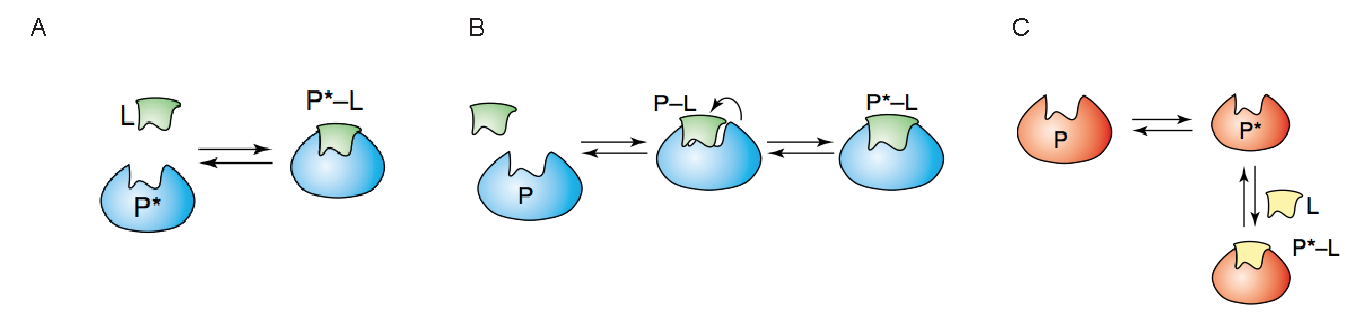
\includegraphics[width=1\textwidth]{images/chap2/figure2_1.pdf} %three modes of binding
   \caption[Three Models of Protein Binding]{ Three models of protein binding. The "lock-and-key" model assumes the protein binding site in a pre-bound state is optimized for the shape of the ligand (A). The "induced-fit" mechanism allows for conformational change after the ligand had bound to optimize shape in a two-step isomerization (B). For the "conformational flexibility" model, the pre-bound structure exists in several isomers which the ligand selects the conformation that complements it's structure (C). Figure adapted from \citep{James:2003ts} }
   \label{fig:abmechanism}
\end{figure}


\subsection{Evidence for Conformational Flexibility}
Conformational flexibility is emerging as an important hypothesis to explain both polyspecificity and changes in affinity between germline and mature antibody sequences \citep{Schultz:2002ef,Notkins:2004iz,James:2003ts,Yin:2003wb,James:2003ip,Foote:1994tr,Romesberg:1998ub,Manivel:2000wk,Yin:2001tq,Nair:2002wz,Jimenez:2003by,Li:2003ic,Mohan:2009hs,Marlow:2010jl,Wong:2011ff,Davies:1996wr,Mohan:2003ko,Wedemayer:1997wn,Zimmermann:2010fb}. The first evidence for conformational isomerism in antibodies was observed through kinetic experiments in which antibodies show a triphasic distribution that, in some cases, appears to reflect the existence of multiple isomers of the unbound antibody in solution, in the pre-equilibrium state \citep{James:2003ip}. To determine the dynamics of the binding process, James and colleagues examined the pre-steady-state kinetics of complex formation between SPE7 and DNP-Ser, as well as between SPE7 and the hapten cross-reactants. The kinetics confirmed the existence of an equilibrium in solution between two preexisting isomers, only one of which bound the haptens. Pre-steady-state binding kinetics were analyzed by monitoring changes in SPE7's intrinsic fluorescence upon rapid mixing with ligand.

In 1997, Wedemayer and colleagues found a structural basis for conformational flexibility observed for germline antibodies \citep{Wedemayer:1997wn}. They solved the crystal structures for a germline antibody with and without its target hapten, and mature antibody with 6 somatic mutations that bound the target hapten 30,000 times stronger than the germline counterpart. They noticed that the rigid-body deviation in the crystal structure was significant between the bound and unbound germline antibody structure indicating a degree of flexibility. In contrast, the mature antibody had less structural deviation upon hapten binding. They showed that the somatic mutations observed in the mature antibody stabilize the binding sites either directly or indirectly by locking the structure into the pre-bound conformation. This was the first indirect evidence showing that germline encoded antibodies may be more flexible than the mature sequences due to the intrinsic properties of the sequence.

More recently, structural studies along with computational tools have corroborated these findings by showing direct evidence that antibodies encoded by germline gene sequences retain flexibility in their HCDR3 loops \citep{Wong:2011ff,Babor:2009it}. For example, Babor et al. redesigned germline or mature HCDR3 loops in antibodies that had been crystallized in free or antigen-bound states \citep{Babor:2009it}. These investigators found that germline gene-encoded HCDR3 sequences are nearly optimal for conformational flexibility. The study, while exceptional in its concept, was limited as the dataset contained many antibody/hapten (non-protein) complexes, which may not reflect the biology of interactions with larger protein targets that are more typical in foreign pathogens. Some antibodies classified as "germline" in the study were not from antigen-na�ve cells. Further, that study exclusively analyzed the HCDR3 loop, not the entire variable region.

Schmidt \textit{et al.} used molecular dynamics simulations and structural analysis to determine how mutations in the antibody variable domain enhance antigen binding to the influenza virus HA protein \citep{Schmidt:2013ka}. In the study, they found two broadly neutralizing antibodies that have branched in lineage from a common intermediate, and an unmutated common ancestor (UCA) in which they obtained high-resolution crystal structures. They found that even though the UCA and mature antibodies have nearly identical binding configurations, the affinity for influenza for the mature antibodies was 40-fold greater than the UCA. Molecular dynamics simulations predicted that the paratope in unbound UCA was not in an optimal conformation for binding, while the mature antibodies had a higher probability of being pre-configured for the influenza HA epitope.

\subsection{Experimental Rationale}
The V\textsubscript{H}-gene encodes the HCDR1, HCDR2, much of the immunoglobulin framework regions and the beginning of the HCDR3 loop. I hypothesized that the conformational flexibility mediating the polyspecificity of germline gene-encoded antibodies is determined at least in part by the heavy chain variable region encoded by the V\textsubscript{H}-gene, considering it makes up a large portion of the structure. The focus of my study was to test this hypothesis using computational design. Specifically, I analyzed the somatic mutations in sets of mature antibodies that derived from the same V\textsubscript{H} gene and for which co-crystal structures with biologically relevant target proteins were available. Sets of mature antibody-antigen complexes incorporating antibodies that derived from a common germline V\textsubscript{H}-gene were input into the \rosetta~"multi-state" design algorithm that recovers the optimal single sequence for an antibody to bind all antigens simultaneously \citep{Babor:2009it,Humphris:2007gq,LeaverFay:2011ji}. The sequences recovered using this protocol would be considered inherently flexible and polyspecific, since they are predicted to accommodate binding to diverse antigens using a structurally diverse set of antibody conformational states.
In contrast, I also tested monospecificity for each antibody by measuring which sequences are preferred during the design towards a single antigen. This is known as the "single-state" design protocol. For any change between the preference for sequence between the multi-state design protocol that considered polyspecificity and the single-state design that considers monospecificity, recapitulates \textit{in silico}, the process of affinity maturation.

Fundamentally, our approach compares germline and mature antibody sequences optimized in nature through evolution and maturation with sequences predicted to be optimal based on \rosetta's energy function applied to a set of co-crystallized antibody/antigen complexes. The power of the present approach is that I predicted germline and mature sequences \textit{in silico} without any prior knowledge of either, which is an important step towards rational antibody design. I would expect that results of this type of analysis will continue to improve as the size of the collection of conformational ensembles available in the Protein Data Bank (PDB) increases and as the accuracy of the \rosetta~energy function continues to improve.

\section{Multi- and Single-State Design of Antigen-Antibody Complexes}
I compiled panels of antigen-antibody complexes from the Protein Data Bank (PDB) in which the antibody heavy chain variable region were encoded by germline V\textsubscript{H}-genes, designated V\textsubscript{H}3-23, V\textsubscript{H}1-69, or V\textsubscript{H}5-51 \citep{Wu:2010dw,Tian:2008vq}. Antigen-antibody complexes were selected only if they contained Homo sapiens or humanized antibodies and the binding partner was a protein antigen. The search of the PDB returns 10, 8 or 3 candidate complexes for V\textsubscript{H}1-69, V\textsubscript{H}3-23, or V\textsubscript{H}5-51 respectively (table \ref{tab:dataset}).

\begin{table}[h]
\centering
\begin{tabular}{llllc}
\toprule
PDB ID & V\textsubscript{H}* Germline & Antibody    & Ligand    & V\textsubscript{H}* Mutations \\
\midrule
2CMR   & 1-69*01      & D5          & gp41      & 6             \\
3FKU   & 1-69*01      & F10         & HA        & 13            \\
3GBM   & 1-69*01      & CR6261      & HA        & 15            \\
3MA9   & 1-69*01      & 8066        & gp41      & 4             \\
3MAC   & 1-69*01      & 8062        & gp120     & 7             \\
3P30   & 1-69*01      & 1281        & gp41      & 20            \\
1G9M   & 1-69*02      & 17b         & gp120     & 21            \\
2DD8   & 1-69*05      & M396        & SARS-RBD  & 5             \\
2XRA   & 1-69*05      & HK20        & gp41      & 14            \\
2XTJ   & 1-69*10      & 1D05        & PCSK9     & 4             \\
2QQN   & 3-23*01      & anti-Nrps-1 & Nrps-1    & 10            \\
2R56   & 3-23*01      & IgE         & BLG       & 23            \\
2VYR   & 3-23*01      & VH9         & MDM4      & 10            \\
3KR3   & 3-23*01      & DX-2647     & IGF-II    & 8             \\
1S78   & 3-23*04      & Pertiuzimab & ErbB2     & 22            \\
2FJG   & 3-23*04      & G6          & VEGF      & 15            \\
3DVN   & 3-23*04      & Apu2.16     & Ubiquitin & 18            \\
3BN9   & 3-23*04      & E2          & MT-SP1    & 5             \\
2B1A   & 5-51*01      & 2219        & UG1033    & 17            \\
2XWT   & 5-51*01      & K1-70       & TSHR      & 8             \\
3HMX   & 5-51*01      & Ustekinumab & IL-12     & 12           \\
\bottomrule
\end{tabular}
\caption[Antibody-antigen test set]{Antibody-antigen test set. Details of the 10, 8, and 3 complexes for V\textsubscript{H}1-69, V\textsubscript{H}3-23, and V\textsubscript{H} 5-51 respectively. The antibodies bind a diverse set of antigens but each share a common germline across a test set. The V\textsubscript{H} mutation count of amino acid mutations away from their inferred germline gene. *Predicted from IMGT}
\label{tab:dataset}
\end{table}



For each panel I compared the mature (somatically mutated) sequence to the inferred germline gene sequence via a multiple sequence alignment (figure \ref{fig:polymethods}A). The number of mutations with respect to the germline sequence range from 4 to 23 mutations with an average of 12.2. All HCDR1, HCDR2, and framework positions that differed from the germline sequence of the common V\textsubscript{H}-gene sequence in at least one position in the multiple sequence alignment were included in the computational design simulations as "variable positions". Note that my study explicitly excluded positions that remained unchanged as no claims can be made with respect to the relevance of these positions for conformational flexibility or polyspecificity. My analysis is limited to antibody regions encoded by the V\textsubscript{H}-gene as only this region can be unambiguously aligned within each set of antibodies. Therefore, I excluded D-gene and J-gene that encode HCDRH3, and antibody light chain positions. The identity and conformation in all variable positions to identify the sequence and conformation that return minimal energy for the given protein backbone of the antibody/antigen complex \citep{Kuhlman:2000tc}. In this work, I used multi-state design \citep{LeaverFay:2011ji} to find a single sequence that minimized energy with all antigens within each V\textsubscript{H} gene-encoded group. To reduce noise in the outcome of the computations, 100 simulations were executed, and results are displayed using WebLogo representation \citep{Crooks:2004do} (figure \ref{fig:polymethods} C).

For a concrete example, consider position 31 (PDB numbering, boxed in \ref{fig:polymethods} C). This position, encoded by V\textsubscript{H}5-51, diverged from a germline serine residue in the sequence for all three complexes. Complexes 2B1A and 2XWT (PDB code) possess an aspartate residue in this position acquired by somatic mutation, while 3HMX has a threonine in the same position. The multi-state design protocol selected the germline residue serine as the energetically most favorable residue out of all 20 possible genetically encoded amino acids when interaction with all three structurally diverse antigens is required. The experiment was repeated as three separate "single-state design" experiments (figure \ref{fig:polymethods}B, right side) to predict the sequences and conformations that minimized interaction energy for each antigen individually. The resulting sequences were compared to both the inferred germline and the mature sequence (figure \ref{fig:polymethods}C). In this experiment position 31 is predicted as an aspartate for complexes 2B1A and 2XWT, and as a threonine for 3HMX, the mature amino acid sequence (data not shown).

For this work, it was important to convert the outcome to a statistical quantitative analysis. Each design outcome is compared to the mature or germline sequence, by computing a bit-score "recovery" measure. The results can either recover towards germline, mature or neither sequences. The bit-score computation I used is described in the methods of the appendix section. The advantage of the bit-score measure in comparison to a more simplistic percentage-recovery is that it analyzes the relative probabilities of all twenty amino acids in a particular sequence position, not just the probability of the correct one. It thereby arrives at an accurate measure of "surprise" of seeing a certain outcome, a normalized measure in information theory that can be readily compared between different experiments. In our experiment high bit-score for the germline sequence indicated that among the 100 designed sequences, germline gene-encoded residues were chosen in a large number of instances (figure \ref{fig:polymethods}D). To facilitate comparison across complexes that have a different number of designed entities considered, I determined the sum bit-scores over all designed positions and normalized the score to fall between 0 and 1 by division with the maximum bit-score that could be achieved, \textit{i.e.}, every amino acid position designed towards a germline or mature sequence.

\begin{figure}[t!]
\centering
 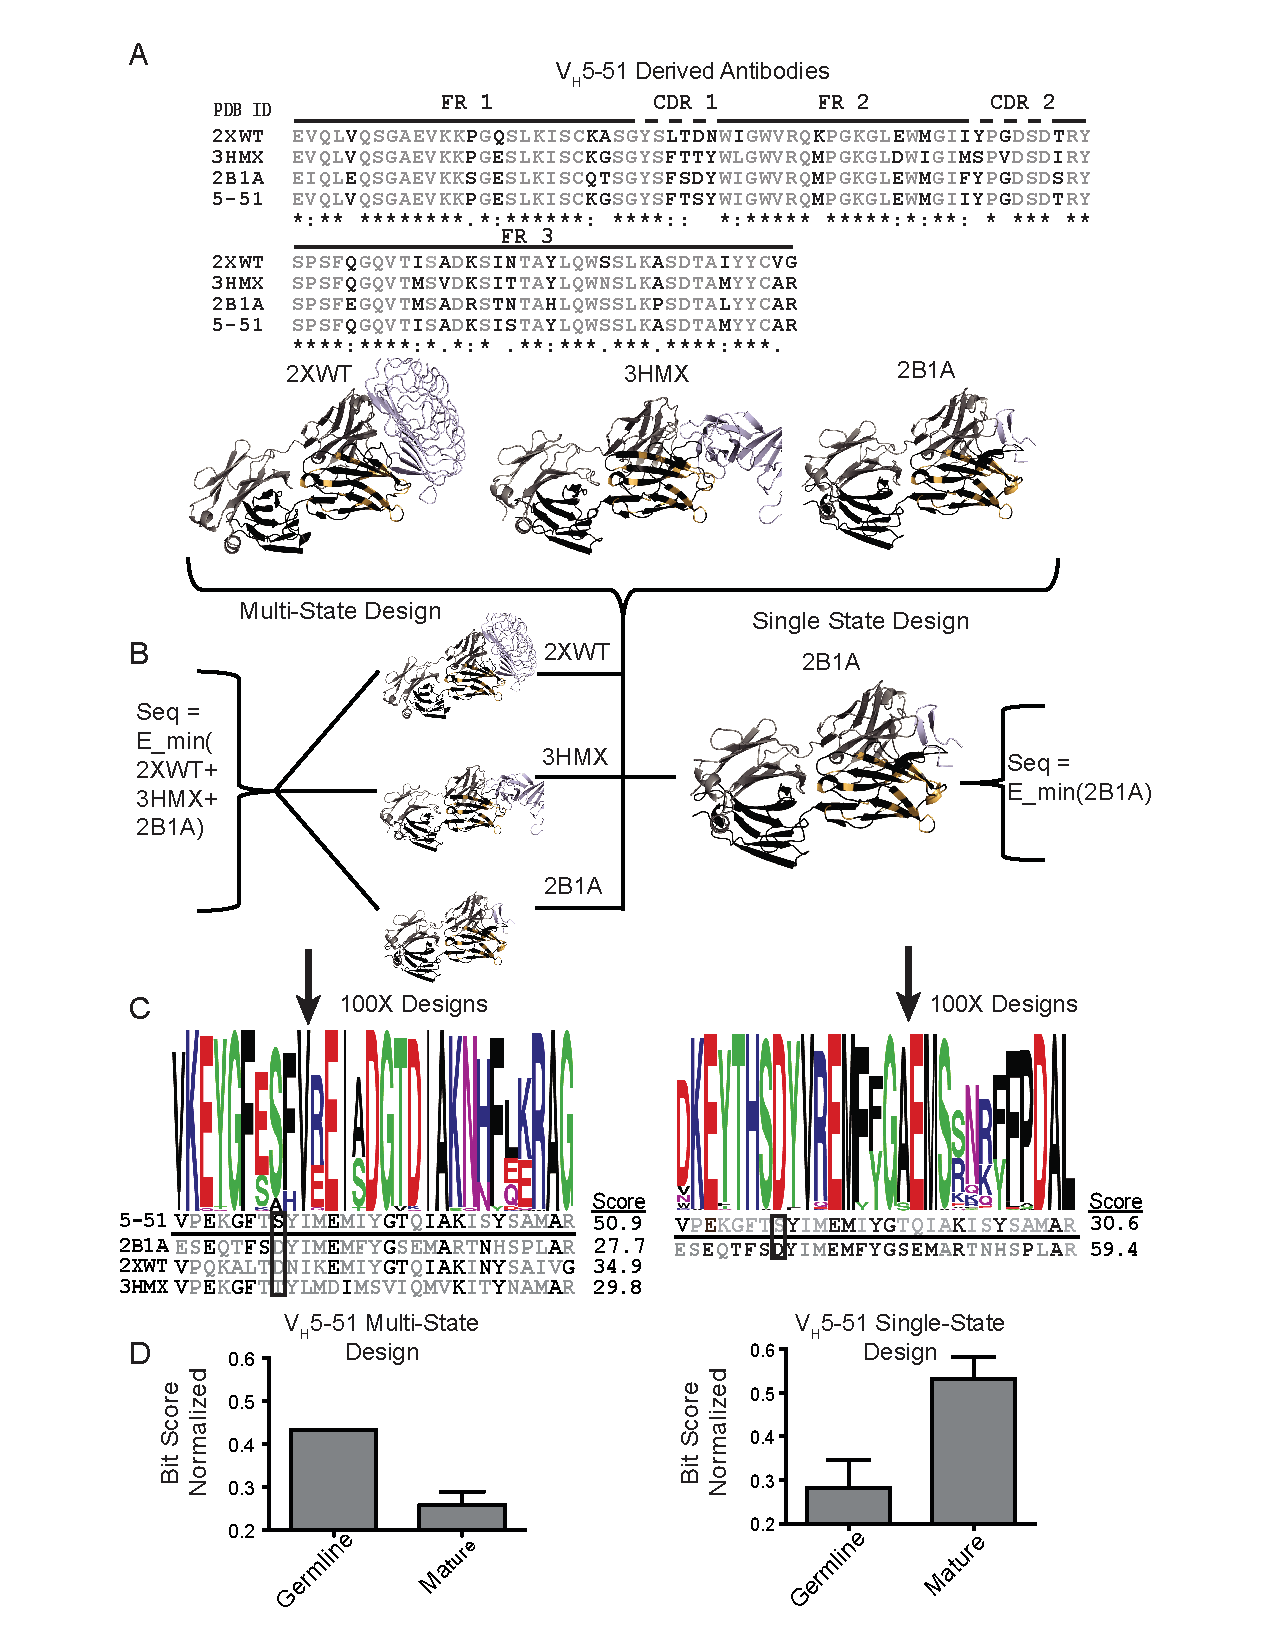
\includegraphics[width=.9\textwidth]{images/chap2/figure2_2.pdf}
   \caption[Multi-State and Single-State Design Methodology]{Multi-state and single-state design methodology. Position candidates were chosen for design if the position differed from the germline sequence in at least one mature complex (A). Co-crystal structures for each complex are shown with designed positions highlighted in gold. Single- and multi-state design schemes are shown (B)  Each position in the sequence logo corresponds to a position conserved for design (C). Bit-scores were determined quantitatively by measuring the frequency of a letter at each position (D).}
  \label{fig:polymethods}
\end{figure}



\section{Specificity Inferred by Sequence Design}
The results of the multi-state design simulations returned sequences that resembled germline gene-encoded sequences more often than mature sequences. This finding was remarkable as no information about germline sequences was input into the simulation. I found that the designed sequences gave normalized bit-scores of 0.54, 0.60, and 0.43 for germline genes V\textsubscript{H}1-69, V\textsubscript{H}3-23, or V\textsubscript{H}5-51, respectively. In contrast, statistically significant reduced bit-scores of 0.48, 0.45, or 0.26 (p < 0.0001) were observed when comparing the designed sequences with the mature genes (figure \ref{fig:polyresults}A).
The single-state redesign of mature antibodies for binding to their associated antigen gave normalized bit-scores of 0.47, 0.43, or 0.28 for comparison with germline gene-encoded sequences and 0.57, 0.54, or 0.53 for comparison with mature sequences of V\textsubscript{H}1-69, V\textsubscript{H}3-23 or V\textsubscript{H}5-51, respectively. In this design experiment, a proclivity to recover the somatically mutated mature sequences was observed (figure \ref{fig:polyresults}A). Given that a normalized bit-score is the preference for each design experiment to match a certain sequence profile, a high bit-score to germline sequence indicates the output matching the germline profile, while a high bit-score to the mature sequence indicates a preference for the mature profile, each design experiment outcome can be measured as a difference in bit-scores (mature - germline). With this definition, a preference for mature sequence gave a positive $\Delta$bit-score, while a preference for germline residues gave a negative $\Delta$bit-score for a given complex - \textit{i.e.}, the $\Delta$bit-score provided an \textit{in silico} predicted metric for antibody optimization for affinity to a specific antigen versus polyspecificty. I observed positive values for single-state design and negative values for multi-state design, indicating a preference for the mature or germline sequences, respectively (figure \ref{fig:polyresults}B, p < 0.0001).

\begin{SCfigure}
   \centering
   \caption[Multi-State Designs Toward the Germline Sequence ]{Multi-state designs toward the germline sequence. Antibodies encoded by the same inferred germline V\textsubscript{H} gene preferred germline sequences when considered in the multi-state design, inferring a more flexible combining site. The bar graph shows the bit-score for each of the three different inferred germline groups and then the sum of the scores in a grouped bar. A perfect design would have a normalized bit-score of 1.0, and summated score of 3.0 for three germline groups. Multi-state design preferred germline sequences for all complexes, while in contrast single-state design preferred mature sequences (A, p<0.0001). The change in bit-score is determined to be the proclivity to either the mature (positive score) or the germline (negative score) sequence. Each complex was assigned a change in bit-score. The change in proclivity between design protocols was significant (B, p< 0.0001). Each complex was scored against mature and germline sequences and a difference was calculated ($\Delta$bit-score). Positive numbers returned showed a proclivity towards mature sequences, while a negative score suggested a design toward germline. A tight correlation was observed (r$^{2}$=0.8263) for the \textit{in silico} predicted optimization for specificity versus polyspecificity ($\Delta$bit-score) and the \textit{in vivo} maturation process (C, plotted as the mutation percentage away from V\textsubscript{H} gene sequence).}
   	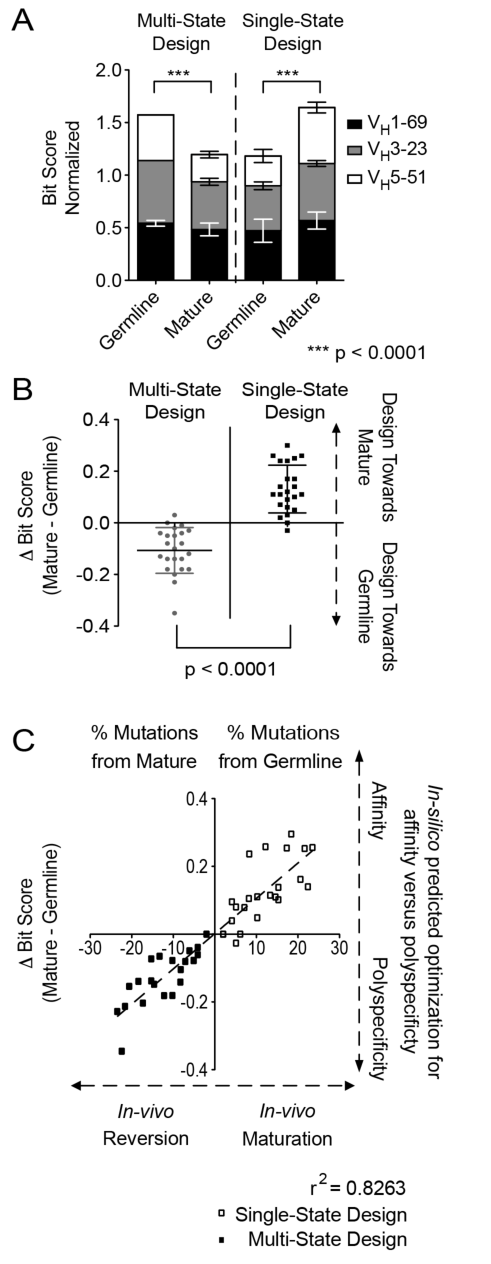
\includegraphics{images/chap2/figure2_3.pdf}
   \label{fig:polyresults}
\end{SCfigure}


\section{Affinity Maturation Correlates with Predicted Affinity}
The number of somatic mutations can be used as a measure of the maturity of an antibody \citep{Briney:2012ib}. Hence, I asked the question if the $\Delta$bit-score, the change in proclivity for a germline or mature sequence, correlated with affinity, \textit{i.e.}, if tendency to recover mature versus germline sequences increased as antibody maturation progressed. Such a correlation would indicate that as antibodies mature, features of the germline sequence critical for polyspecificity are replaced with features critical to recognize one target antigen. Figure \ref{fig:polyresults} C shows the somatic mutation percentage of antibodies in each complex as a metric  for ``\textit{in vivo} maturation'' correlated with the $\Delta$bit-score as a metric for "\textit{in silico} predicted optimization for affinity versus polyspecificty". For positive $\Delta$bit-scores, the mature sequence was preferred, indicating a preference for specificity. For negative values, the germline sequence, and hence polyspecificity was preferred. The correlation coefficient for the ``\textit{in vivo} affinity maturation'' and "\textit{in silico} predicted optimization for affinity vs. polyspecificity" was 0.83.

\section{Backbone Conformational Space for Germline Sequences}
Torsional phi-psi angles in the protein backbone were compared across the sets of experimental structures for positions that recovered to germline sequence for multi-state design and those positions that recovered to a non-germline sequence. I found that positions that converted back to germline in multi-state design, \textit{i.e.}, positions critical for conformational flexibility according to the simulation, had a deviation of 19.6$^\circ$ $\pm$ 2.0$^\circ$ across beta-sheet phi-psi torsion angles. Sequence positions that did not recover to a germline gene-encoded amino acid had a reduced deviation 15.5$^\circ$ $\pm$ 1.5$^\circ$ for beta-sheet backbone torsion angles (p = 0.099) (figure \ref{fig:polyfw} A-C). Considering the limited range for beta-sheet backbone torsion angles, I don't expect large deviations. For reference, all framework residue beta-sheets in antibody-antigen complexes across my dataset have an average phi-psi deviation of 18.7$^\circ$ $\pm$ 0.9$^\circ$.

\begin{SCfigure}
   \centering
   \caption[Phi-Psi Variances for Framework Residues]{Phi-psi variances for framework residues. The degree of structural variation of the framework residues were measured as the standard deviation of the phi and psi angles over each residue position. Side view of immunoglobulin fold for V\textsubscript{H}5-51 complexes aligned by framework residues. Beta-sheets included in the analysis are shown as a cartoon representation, while loop regions are in a transparent ribbon representation. Framework 1 is shown in brown, HCDR1 in green, framework 2 in black, HCDR 2 in magenta, and framework 3 in cyan (A). Same as (A) but top down view (B). The standard deviations of the phi-psi angles of each framework position were binned into either a residue that was found to be critical for polyspecificity (recovered to germline) or a residue that was not recovered to germline in multi-state design.  For each position, the phi-psi angles were averaged, and the standard error of the mean was calculated. An average of 19.6$^\circ$ $\pm$ 2.0$^\circ$ for germline recovered residues and 15.47$^\circ$ $\pm$ 1.5$^\circ$ for non-germline recovered residues supporting our hypothesis that residues which enable polyspecificity alter beta-sheet packing to a greater degree than residues that do not. The axis is normalized to 18.7$^\circ$ $\pm$ 0.9$^\circ$, the average deviation for all beta-sheet framework positions (C).}
   	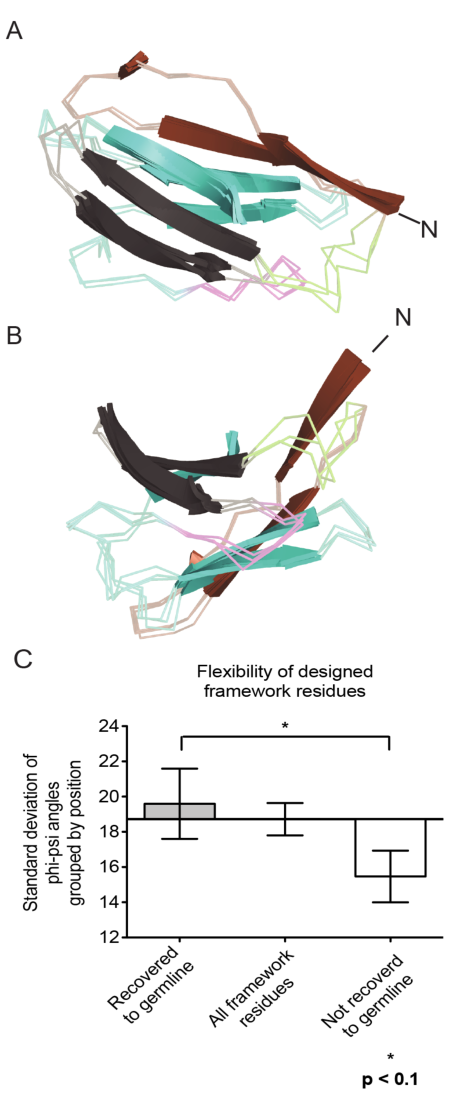
\includegraphics{images/chap2/figure2_4.pdf}
   \label{fig:polyfw}
\end{SCfigure}


\section{Impact of Residue Environment on Specificity}
Figure \ref{fig:polyenv} maps each amino acid position encoded by the V\textsubscript{H} gene segment onto the immunoglobulin fold using a custom Collier de Perles representation, as described by Ruiz and Lefranc \citep{Ruiz:2002jd}. I modified the output to distinguish positions by location in the interface with the antigen and the degree of burial. I correlated these metrics to the bit-score at a per-residue level. Each residue given is in IMGT numbering.

For multi-state design (figure \ref{fig:polyenv} A-C), 33 out of a possible 46 of the designed interface residues (72\%) contributed to polyspecificity, \textit{i.e.}, recovered to germline sequence with a normalized bit-score > 0. Remarkably, also 41 out of 77 residues outside the interface (53\%) recovered to germline. Residues 25, 40 and 105, far removed from the interface, recovered perfectly (normalized bit-score = 1) in at least two of the three germline gene test sets. These residues are highly buried, with a neighbor count score of 13.3 $\pm$ 0.5. The intermediately packed residues 17, 51, 70, and 71, with an average neighbor score of 8.6 $\pm$ 2.2 neighbors, were predicted to contribute to polyspecificity, even though they lie in distal positions from the antigen-binding site. The interface residues 35, 63, 64, and 82 were found to contribute to polyspecificity in two out of the three germline gene test sets. A conserved serine, which was found in all three germline sequences at position 36 in the CDR1, was the only residue identified as critical for polyspecificity in all three germline genes.

In contrast, for single-state design, it is more difficult to deduce overall trends for any specific position as the paratope is altered in each antibody and the recognized epitopes cover diverse structural space. Generally, when each complex was considered individually, 214 designed interface residues recovered to their mature sequence out of a possible 340 designed amino acids, indicating their importance for recognition of, and affinity for binding to, the specific antigen (63\%, figure \ref{fig:polyenv} D-F). When non-interface residues were considered, 411 out of a possible 699 designed residues recovered to their mature sequence (59\%).

Residues that were found to be critical for polyspecificity, \textit{i.e.}, reverted to germline in multi-state design, differed substantially for each germline gene test set considered. For the V\textsubscript{H}1-69 gene derived antibodies, all of the residues in the HCDR2 loop contributed to binding interactions in the single-state but not the multi-state design. In contrast only G63 and T64 residues contributed in the multi-state case but not in single-state designs. Residue L50 was recovered in all single-state complexes but was not critical for multi-state design. For the V\textsubscript{H}3-23 gene, residues A55 and Y66 were not recovered in multi-state design but were found to be important for high affinity in single-state design. For the V\textsubscript{H}5-51 complexes, non-interface residues P15, M53 and A80 were not recovered in multi-state design but were found to be critical in single-state design. HCDR2 was found to be critical in single-state design for all V\textsubscript{H}5-51 complexes.

\begin{figure}
\centering
 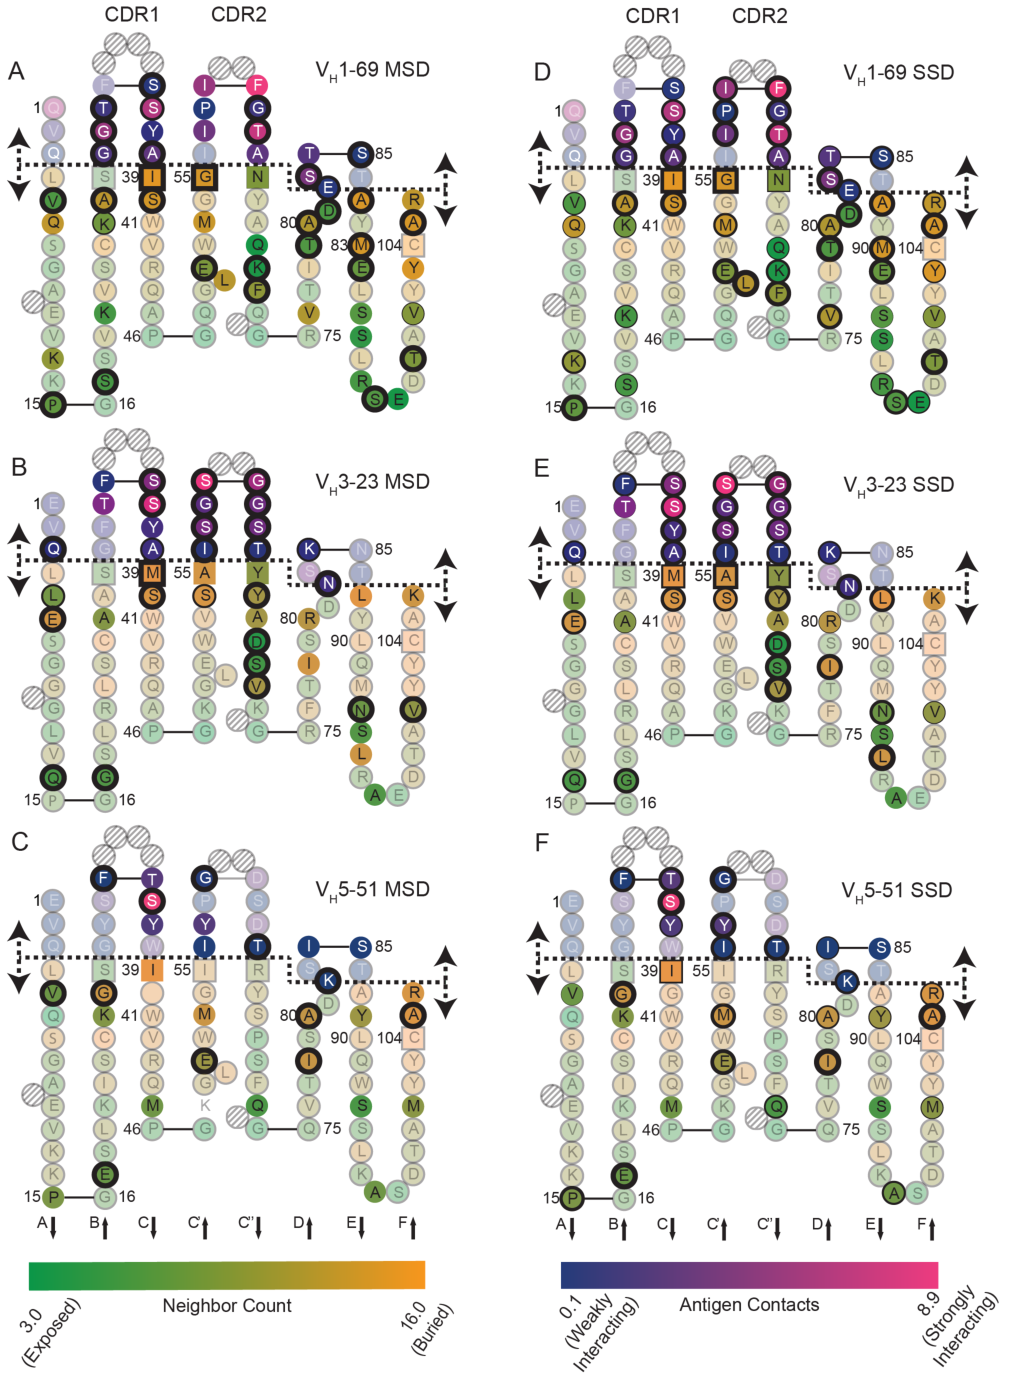
\includegraphics[scale=.7]{images/chap2/figure2_5.pdf}
   \caption[Colliers de Perles Representation of V\textsubscript{H} Gene Segments ]{Colliers de Perles reepresentation of V\textsubscript{H} gene segments. The 98 amino acids present in V\textsubscript{H}1-69, V\textsubscript{H}3-23, or V\textsubscript{H}5-51 are shown in a Collier de Perles two-dimensional representation and numbered according to the IMGT numbering scheme 37. Hatched circles are missing residues according to the IMGT numbering scheme and are shown to make graphs consistent. Square boxes represent the boundary between framework and CDR loops. A dashed line is shown for the interface. Interface residues are colored with a blue-pink gradient indicating a numerical antigen contact score defined by a change in neighbors between the free and bound complex. Non-interface residues are colored with a green-orange gradient according to their degree of burial defined through a neighbor count. A, B, C show the germline sequence represented in the immunoglobulin fold with the thickness of each line representing the design bit-score for that position relative to the germline sequence for multi-state design. D, E, F the thickness of the line corresponds to the mature sequence bit-score averaged over each complex.}
  \label{fig:polyenv}
\end{figure}


\section{Mature Sequence Bias}
\label{sec:maturebias}
To understand some of the trends described above more quantitatively, I determined for each residue in each antibody/antigen complex if it was part of the interface, \textit{i.e.}, directly engaging the antigen. For this purpose the change in neighbor count between unbound antibody and bound antibody/antigen complex score was measured, and positions with a change larger than 1.0 were classified as "interacting residues". Next, I counted how often a residue position appeared in the interface within each set of antibody/antigen complexes. Positions were binned as occurring in the ensemble interface never, once, two-four times, or more than four times and average bit-scores were compared (figure \ref{fig:polymsb}). I found a general trend for interface ensemble size correlating with interface ensembles sampled. For the set of structures derived from V\textsubscript{H}3-23, which contained a total of 8 complexes, I found that residue positions that are never found in the interface gave an average bit-score of 2.3 $\pm$ 0.4. If a residue position was found only in one interface, the average bit-score dropped to 1.2 $\pm$ 1.1. As residues were found more frequently at the interface between 2-4 complexes, and 5-8 complexes, the average bit-score increased to 2.5 $\pm$ 0.8 and 3.6 $\pm$ 0.7 respectively. For the 10 V\textsubscript{H}1-69 complexes, an average bit-score of 2.3 $\pm$ 0.3 was observed for residues that were never found in the interface. If a residue was only found in the interface once, the average bit-score dropped to 1.9 $\pm$ 1.0. For interface occurrences between 2-4 and 5-8, I found the average bit-score to increase to 2.6 $\pm$ 0.7 and drop to 0.8 $\pm$ 0.4 respectively. Due to the limited number of residues occurring in multiple interfaces, a significant change in bit-score between each grouping was not observed for V\textsubscript{H}1-69 (p= 0.1844) and V\textsubscript{H}3-23 residue positions (p=0.2007).

\begin{figure}[!t]
   \centering
   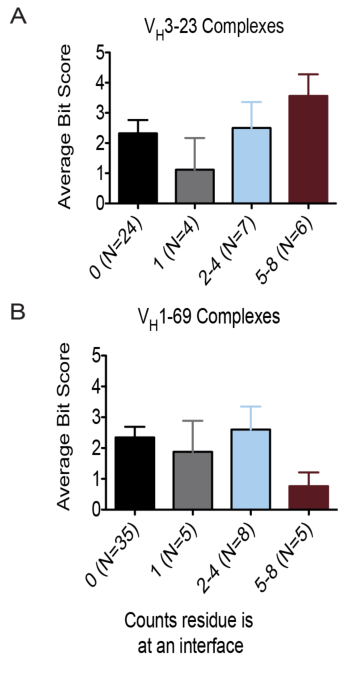
\includegraphics{images/chap2/figure2_6.pdf}
   \caption[Interface Occurrences Affect Germline Sequence Recovery]{Interface occurrences affect germline sequence recovery. For V\textsubscript{H}3-23 (A) and V\textsubscript{H}1-69 complexes (B), I binned each residue position into how many times it occurred in an interface (interface ensembles). Most designed positions never occurred in an interface. As their occurrences became more frequent, I observed a trend for increasing the recovered germline residue. This trend fell off for V\textsubscript{H}1-69 complexes (B) for positional occurrences between 5-8 interfaces.}
   	   \label{fig:polymsb}
\end{figure}


\section{Evolutionary Sequence Bias}
\label{sec:evobias}
I expected the result of multi-state design to deviate from germline in cases where alternate amino acids are compatible with the conformational space and binding modes observed in the ensemble of structures. Alternative amino acids might be tolerated but are not observed in evolution - "evolutionary sequence bias". To test this hypothesis, I reverted each position back to germline and compared the energetic change with the favored residue returned by multi-state design. Using reference energies, \rosetta~facilitates the direct comparison for energies between different residue types \citep{Kuhlman:2003kp}. For complexes derived from V\textsubscript{H}5-51, all positions in which the germline residue were not chosen in at least 10\% of the 100 simulated models were forced into the germline identity (figure \ref{fig:polyesb} A, x-axis). The difference in average energy of the germline sequence at that position from the average energy of the residue returned by multi-state design was calculated (y-axis). For each position, if positive values were returned for all three complexes, \rosettadesign~would most likely place a non-germline amino acid at that position. If negative values were returned for all three complexes, \rosetta~would most likely place a germline amino acid at that position. I found that, in most cases, the energetic contribution of the designed amino acid is not significantly more stabilizing than the germline amino acid, \textit{i.e.} the germline sequence is tolerated as well. Only positions 52, 76, 88, and 98 gave a significant energy increase for the germline sequence in at least one complex. Changes in energy were classified as significant if larger than 0.7 \rosetta~energy units (REU, horizontal dashed line). This threshold was derived from the average difference in energy between the germline and mature residue (0.7 $\pm$ 0.2 REU, data not shown). For Figure \ref{fig:polyesb}B, a multiple sequence alignment is given as a reference, where each position that was considered in multi-state design is highlighted in bold while each position that recovered well to the germline sequence is highlighted in green.

\begin{figure}[!t]
   \centering
   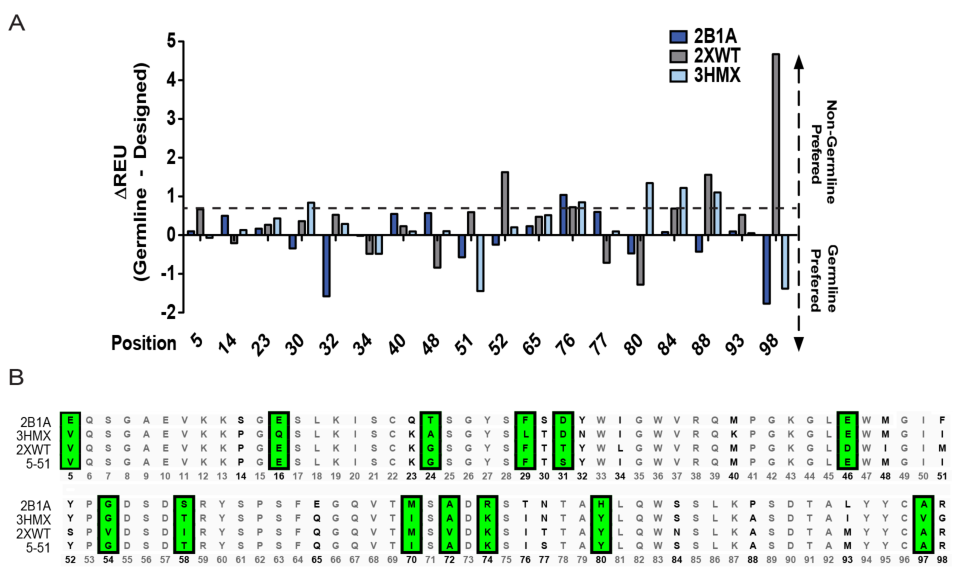
\includegraphics[width=\columnwidth]{images/chap2/figure2_7.pdf}
   \caption[\rosetta~Multi-State Design Solutions]{\rosetta~multi-state design solutions. I evaluated a complete germline reversion of V\textsubscript{H}5-51 sequence versus the sequences output by multi-state design. (A) Consideration of positions in which the multi-state design algorithm chose a non-germline amino acid for at least 10\% of the models where evaluated. The difference in energy of the germline sequence and the multi-state design solution sequence is shown for each position. Bars above 0 represent the multi-state design sequence preferred while bars below the line represent the germline amino acid preference. The horizontal dashed line at 0.7 \rosetta~energy units (REU) shows the average energy difference between the germline and mature sequence and is represented as a marker for sequence tolerance. (B) The multiple sequence alignment for each V\textsubscript{H}5-51 complex is shown and compared with the germline sequence. Sequences highlighted in bold were considered for design. Sequences highlighted in green are positions in which the multi-state design algorithm chose the germline amino acid as the design solution. The numbers in the bottom row are the alignment-numbering scheme of each position and correspond to the position numbers in (A).}
   	   \label{fig:polyesb}
\end{figure}



\section{Discussion}
\subsection{Limitations of Computation}
\label{sec:limits}
I recognize several important limitations of my study: \begin{enumerate}
\item I assumed that the \rosettadesign~protocol determined the optimal sequence for any given design challenge. While it has been demonstrated that \rosettadesign~typically recovers close-to-optimal sequences \citep{Kuhlman:2000tc}, inaccuracies in the scoring function and limitations in the sampling algorithm will introduce errors. In the future, this limitation could be reduced by improvements applied to the energy function and comparing the results obtained with complementary energy functions. I assumed that the finite and small set of antibody conformations observed in the set of co-crystallized mature antibodies completely describes the conformational flexibility of the germline gene-encoded antibody (finite ensemble bias). While I used the largest ensembles available (10, 8, and 3 antigen-antibody complexes), this assumption must be wrong, introducing a bias. For example, assume there is a sequence position that is part of the paratope in only one of the n complexes. In this antibody, a somatic mutation occurred at this position greatly increasing affinity to the antigen. The somatically mutated amino acid is however compatible with all other n-1 complex structures. In such a scenario the multi-state design algorithm will recover the somatically mutated instead of the germline amino acid. Here, I found that as a residue was more often part of the paratope, it became more likely to be recovered to the germline sequence. This finding might be due to the fact that a critical conformation that the germline antibody needs to adopt was not represented in the ensemble (for framework residues) or the epitope needed for recognition by a critical germline amino acid represented in the ensemble.

\item I assumed that the germline gene-encoded antibodies were able to adopt the conformations of each of the mature antibodies derived from it. This assumption is important, as crystal structures of the "true" germline antibody in complex with the antigen are generally not available. While this assumption is expected to be correct for the majority of cases, notable exceptions are discussed in the literature \citep{Yin:2003wb,Li:2003ic,Wedemayer:1997wn,Sethi:2006dq}.

\item It is not guaranteed that only the germline amino acid is compatible with all conformations adopted by mature antibodies. Rather, it is likely that for some positions alternative amino acids are plausible or even better in realizing the conformational flexibility needed. The germline sequence observed in nature is optimized in evolution and clearly works, but does not need to be perfect in all positions. In such a scenario, multi-state design could return amino acids that deviate from germline (evolutionary sequence bias). Conversely, the mature sequences observed in the co-crystal structures are not guaranteed to be the perfect sequence for high affinity. In some positions a somatic mutation might have introduced a better amino acid but is not the "true" best option. Some somatic mutations might have occurred by chance and do not contribute to affinity maturation. Some positions might not have experienced somatic mutations but still favorable mutations exist. In all these cases I expect the single-state design to deviate from the mature sequence observed in the co-crystal structure (evolutionary sequence bias).

\item The imperfect nature of the \rosetta~scoring function will not yield 100\% agreement with natural phenomenon \citep{Kuhlman:2000tc}. Importantly, water coordination can often be important in antibody-antigen binding sites. However, \rosetta~is currently being developed to include tools with explicit solvent models \citep{Lemmon:2012ku}.



\end{enumerate}
It is important to understand these biases and limitations to arrive at an accurate interpretation of the results. Given these known limitations, I expected imperfect agreement of \textit{in silico} predicted and natively observed mature and germline gene-encoded antibody sequences. Nevertheless, I found a remarkably high correspondence of residues designed for polyspecificity in a blinded fashion and the amino acids encoded by germline genes.

\subsection{Interpretation}
Germline gene-encoded sequences for commonly used V\textsubscript{H} segments are hypothesized to possess high conformational flexibility making them ideal for binding diverse antigens, \textit{i.e.}, being polyspecific. During antibody maturation, somatic mutations are introduced that increase affinity for a specific target in part by adding attractive interaction to the antigen (increasing enthalpic gain) and in part by locking the conformation critical for interaction with the specific antigen (reducing entropic cost). Here I tested this hypothesis by analyzing three sets of antibodies, each derived from a commonly used V\textsubscript{H} gene and each co-crystallized with a protein target in its antigen-specific binding conformation.

I chose to not directly compare conformational flexibility for germline and mature antibodies. While this approach may be feasible in general through predicting the accessible conformational space using molecular dynamics \citep{Wong:2011ff}, it is challenging to achieve complete sampling of large conformational spaces that include the entire immunoglobulin framework. To circumvent this problem, I chose to solve the inversely related protein design problem, which was to study amino acid sequences that are consistent with the conformational space seen in antibody/antigen co-crystal structures. This approach is complementary and potentially superior as it replaces sampling of the large conformational space in antibody backbone regions with solving the better understood ranking of amino acid sequences, given a certain antibody/antigen complex conformation. Specifically, I employed multi-state design to find single amino acid sequences that were compatible with the multiple conformations of antigen combining sites.

Computational tools to design multi-specific proteins were first described by pioneering work in the Kortemme laboratory \citep{Babor:2009it,Humphris:2007gq}. In parallel, Leaver-Fay and colleagues developed a general algorithm for multi-state design in the \rosetta~framework, in which they designed one protein to interact with non-native targets \citep{LeaverFay:2011ji}. I used the latter tool to design antibody sequences that are optimal for facilitating interactions to: \begin{enumerate}
\item Multiple and diverse antigens, or
\item A single specific antigen.
\end{enumerate}

In the absence of \textit{a priori} knowledge of the germline or mature sequences or the mechanism of antibody maturation through somatic mutations, multi-state design of one antibody to recognize several target proteins recovered sequences similar to those encoded by the inferred germline gene segment. When designing the same antibody to recognize one specific target, the sequence recapitulated the mature antibody sequence. This trend correlated tightly with the divergence of the mature sequence from the inferred germline sequence, \textit{i.e.}, the more somatic mutations an antibody contained, the more reversions to germline needed in order to facilitate interactions to multiple antigens.

Use of a computational tool to approach questions regarding polyspecificity as a function of protein sequence is advantageous, as the \rosettadesign~algorithm is able to rapidly enumerate the effect of multiple simultaneous mutations in sequence space for the entire heavy chain variable region. This task is quite difficult if not impossible to complete experimentally at this scale. In this manner, conformational flexibility in the framework regions, HCDR1, and HCDR2 can be tested in a holistic model. All mutated positions in the V\textsubscript{H} gene segment were considered simultaneously, including the effect of interactions between different domains in the antibody, thus revealing the role of interface and non-interface residues in both poly- and monospecificity. Because this approach considers multiple antibodies of variable conformation at once, each with a distinct binding mode, the multi-state design algorithm predicts sequences that are inherently flexible and capable of adopting the diverse set of conformations needed to bind to multiple antigens.

Harindranath and colleagues demonstrated that polyspecific antibodies were encoded largely by germline gene sequences \citep{Harindranath:1993ty}. Romesberg and Spiller presented structural evidence for flexibility in germline gene-encoded sequences \citep{Romesberg:1998ub}. In addition, Schmidt et al. correlated mature sequence to rigidity of the paratope \citep{Schmidt:2013ka}. Taken together, these data suggest conformational flexibility coupled with pre-sampled conformations of the target binding site as the underlying mechanism for polyspecificity \citep{Wedemayer:1997wn}. Here, I used a multi-state design algorithm to assess the contribution of the V\textsubscript{H} gene segment to specifying an antibody with conformational flexibility, preorganization, and polyspecificity. I found that this property is largely attributed to antibody sequences in the germline gene repertoire, since designing antibodies for polyspecificity, sequences recovered germline gene-encoded sequences, while designing antibodies for monospecificity to a single target, returned sequences similar to the mature antibody. This trend increased in strength the higher the number of somatic mutations that had accumulated, \textit{i.e.}, the further optimized the antibody had become. Importantly, the effect is not limited to the HCDR3, which often contributes much to antibody specificity. I obtained the same finding to be clearly measurable throughout HCDRs 1 and 2 as well as the immunoglobulin frameworks. I found each germline V\textsubscript{H} gene to encode a set of amino acids that enabled polyspecificity in a distinct manner. These positions were present not only in the paratope, but also in the buried or semi-buried positions of the immunoglobulin frameworks (figure \ref{fig:polyenv}). I expect, that with an increasing number of antibody-antigen complexes in the PDB it will become easier to discern general trends.

I conclude that conformational flexibility in the beta-sheet framework is critical for changing critical regulators of the conformation of the paratope - \textit{i.e.}, the takeoff and landing angles of HCDR loops, thereby enabling the paratope of germline antibodies to assume multiple conformations. Accordingly, I find that residues that contribute the most to polyspecificity contain larger deviations of their phi-psi torsion angles (figure \ref{fig:polyfw}). During antibody maturation, mutations in these positions likely lock in the target-specific framework conformation, reducing the entropic cost of target binding. Somatic mutations in the paratope, for example within HCDR1 and HCDR2, can directly increase affinity to a target (enthalpic contribution to free energy), or lock in a conformation that recognizes the target (entropic contribution to free energy). I found that on average 62\% of residues in the paratope and 42\% of residues in the framework were important for changing the binding pattern of the antibody from polyspecificity to recognition of one specific target (figure \ref{fig:polyenv}).

I identified at least four specific scenarios in which current datasets are limiting for informing design efforts:
\begin{description}

\item[The first scenario] involves a framework position that does not interact with the epitope in any of our tested complexes. For this position, the germline residue, and only the germline residue, is capable of adopting the phi-psi angles in order to accommodate the flexibility needed for the binding site. Multi-state design likely designs in the germline residue for each simulation. I then observe agreement between \textit{in silico} design and natively observed sequence for a majority of the designed positions (figure \ref{fig:polyresults}).

\item[The second scenario] involves a framework position that also lies distal from the epitope. In this scenario, the germline residue but also other amino acids are compatible with the observed conformations since they both contain properties to adopt the phi-psi angles necessary to accommodate the flexible binding site. For this scenario, I expect \rosetta's multi-state design algorithm to pick one of the compatible amino acids, not necessarily the germline gene-encoded one. This outcome can occur either because the conformational ensemble is incomplete or because of the evolutionary sequence bias. I find that both biases contribute to ambiguity. Residues that are never found in the interface give modest recovery to germline sequences being either "hit-or-miss" (finite ensemble bias, figure \ref{fig:polymsb}), and residues that are reverted to an amino acid different from that encoded in the germline are not significantly better in energy score than the germline encoded amino acid (evolutionary sequence bias, figure \ref{fig:polyesb})

\item[The third scenario] concerns residues that are at part of the paratope in only one instance. If the mature residue forms critical interactions that minimize the free energy of binding in this one complex, while in all other complexes the residue is not part of the paratope and the mature amino acid seen for the one complex is compatible with the backbone confirmation, \rosetta~will choose the mature residues from the first complex also in multi-state design mode. I observed this trend, especially for V\textsubscript{H}3-23 complexes. If a residue was found in only one interface (figure \ref{fig:polymsb}), that position tended to have a low recovery to the germline sequence.

\item[The last scenario] deals with positions that are part of the paratope multiple times and that experience frequent somatic mutations. As positions are found to be more frequently in interface ensembles, the germline recovery increases as these positions become more important to facilitating direct interactions with their antigen (figure \ref{fig:polymsb}). These residues contribute to polyspecificity by being the preferred residue in interaction with multiple antigens, rather than facilitating binding by altering beta-sheet packing.
\end{description}

\section{Conclusions and Future Directions}
These results suggest that the naturally occurring antibody maturation process can be recapitulated or reversed at least partially \textit{in silico}, opening exciting new avenues for antibody engineering work. Further, my results suggest the applicability of multi-state design to engineer polyspecific antibodies, exploring another important strategy for designing broadly neutralizing antibody therapeutics. Traditional antibody engineering approaches emphasize isolating monoclonal antibodies that are highly specific for a given antigen, relying on display techniques in which emphasis typically is placed only on HCDR loop design. The method described here considers the entire antibody variable region during design, including critical framework residues that allow for conformational flexibility and contribute to polyspecificity. Considering that I found that up to 64\% of framework and HCDR residues may contribute to binding and specificity, computational design will be invaluable to rapidly enumerate the large sequence and structural space of residues that can contribute to breadth of binding diverse targets.



\chapter{HIV NEUTRALIZING ANTIBODIES IN HIV NA�VE DONORS}
\section{Introduction}
\begin{figure}
   \centering
   \includegraphics[width=.9\linewidth]{images/chapter3/figure3_1.pdf} % requires the graphicx package
   \caption[Current Sequencing Technologies]{Current sequencing technologies. On the x-axis is the current read length for each sequencing platform. The y-axis is the bases per run. Each point is a new iteration of that platforms sequencing read length and coverage. HiSeq has the most coverage with relatively short read lengths. Figure adapted from \citep{developmentinNGS:2012bs} }
   \label{fig:figure3_1}
\end{figure}

\begin{table}
\centering
\resizebox{.99\linewidth}{!}{
\begin{tabular}{llllcc}
\toprule
\textbf{Platform}   & \textbf{Instrument}      & \textbf{Year} & \textbf{Reads per run} & \textbf{Read length (mode or average)} & \textbf{Bases per run (gigabases)} \\
\midrule
Sanger & 3730xl          & ND   & 96            & 800                           & 0.0000768                 \\
454        & GS20            & 2005 & 200000        & 100                           & 0.02                      \\
454        & GS FLX          & 2007 & 400000        & 250                           & 0.1                       \\
454        & GS FLX Titanium & 2009 & 1000000       & 500                           & 0.45                      \\
454        & GS FLX+         & 2011 & 1000000       & 700                           & 0.7                       \\
454        & GS Junior       & 2010 & 100000        & 400                           & 0.04                      \\
IonTorrent & PGM 314 chip    & 2011 & 100000        & 100                           & 0.01                      \\
IonTorrent & PGM 316 chip    & 2011 & 1000000       & 100                           & 0.1                       \\
IonTorrent & PGM 318 chip    & 2011 & 5000000       & 100                           & 0.5                       \\
IonTorrent & PGM 318 chip    & 2012 & 5000000       & 200                           & 1                         \\
IonTorrent & PGM 318 chip V2 & 2013 & 5000000       & 400                           & 2                         \\
IonTorrent & Proton PI       & 2012 & 50000000      & 200                           & 10                        \\
Illumina   & GA              & 2008 & 28000000      & 35                            & 1                         \\
Illumina   & GA II           & ND   & 100000000     & 50                            & 5                         \\
Illumina   & GAIIx           & 2009 & 440000000     & 75                            & 33                        \\
Illumina   & GAIIx           & 2011 & 640000000     & 75                            & 48                        \\
Illumina   & GAIIx           & 2012 & 640000000     & 150                           & 95                        \\
Illumina   & HiSeq 2000      & 2010 & 2000000000    & 100                           & 200                       \\
Illumina   & HiSeq 2000      & 2011 & 3000000000    & 100                           & 600                       \\
Illumina   & HiSeq 2500 RR   & 2012 & 600000000     & 150                           & 180                       \\
Illumina   & MiSeq           & 2011 & 30000000      & 150                           & 4.5                       \\
Illumina   & MiSeq           & 2012 & 30000000      & 250                           & 8.5                       \\
Illumina   & MiSeq           & 2013 & 30000000      & 300                           & 15                        \\
SOLiD      & 3               & ND   & 320000000     & 50                            & 16                        \\
SOLiD      & 4               & ND   & 2000000000    & 50                            & 100                       \\
SOLiD      & 5500xl          & 2011 & 3000000000    & 60                            & 180                       \\
SOLiD      & 5500xl W        & 2013 & 3000000000    & 75                            & 320                       \\
PacBio     & RS C1           & 2011 & 36000         & 1300                          & 0.045                     \\
PacBio     & RS C2           & 2012 & 36000         & 2500                          & 0.090                     \\
PacBio     & RS C2 XL        & 2012 & 36000         & 4300                          & 0.155                     \\
PacBio     & RS II C2 XL     & 2013 & 47000         & 4600                          & 0.216                    \\
\bottomrule
\end{tabular}}
\caption[Current HTS Sequencing Platforms]{Figure adapted from \citep{developmentinNGS:2012bs}}
\label{tab:table3_1}
\end{table}
\chapter{Redesign of A Long HCDR3 Antibody}
\label{chap:chapter4}
\section{Introduction}
Recent studies described the isolation of a number of human monoclonal antibodies (mAbs) with broad and potent neutralizing activity, many of which exhibit unusual features \citep{Bonsignori:2011dq,McLellan:2011dg,Walker:2009cd,Walker:2011ew}. As discussed in the chapter \ref{chap:chapter1}, broadly neutralizing antibodies to HIV generally contain high levels of somatic mutations or exceptionally long HCDR3 lengths. The V2/V3 neutralizing class of anti-HIV antibodies which includes PG9, PG16, CH01, CH04, PGT141 and PGT145 all have a long heavy chain complementarity determining region 3 (HCDR3) and possess unique structural elements that interact with complex protein and glycan features reaching past a large bulk of complex and high mannose glycans to interact with a short segment termed strand-C5. These antibodies share similar neutralization sensitivity including glycan knockouts and strand-C point mutations that interact with interface residues \citep{DoriaRose:2012if,Doores:2010gn}.  For PG9 and its clonally related sibling PG16, crystal structures have been solved in complex showing that these antibodies both engage the epitope with their HCDR3 loop in a similar ways with the exception of glycan interactions \citep{Pancera:2013ev}. While PG16 prefers hybrid type glycans at position N173 (HXBc2 numbering), PG9 has little dependence.

\subsection{Experimental Rationale}
As an extension of my work in chapter \ref{chap:chapter3} that considers antibodies with exceptionally long HCDR3s, I chose to pursue a redesign study of the broadly neutralizing antibody PG9. This allowed me to ask relatively simple questions that may have broad and far-reaching implications for antibody and vaccine design. Is the native sequence of PG9 optimal for binding and neutralization potency? PG9 and PG16 converge on structure and binding modes but they are encoded by different sequences. Therefore, I hypothesized that the HCDR3 loop of PG9 could be redesigned to achieve improved affinity of binding, increased potency, and breadth of neutralization for diverse HIV strains.

There has already been precedent for chimeric antibodies of PG9/PG16 where a motif from PG16 responsible for the recognition of complex type glycans was transposed onto PG9 in order to increase potency and breadth by allowing PG9, which initially had no preference for complex type glycans at position 173, to bind those glycan types with stronger affinity, while retaining PG9s ability to bind high mannose type antibodies. This chimeric antibody extended the breadth of PG9 with a small subset of mutations on the light chain CDR3 loop termed PG9-RSH \citep{Pancera:2013ev}.

In addition, NIH45-46, a broadly neutralizing mAb that shows structural mimicry for CD4 and closely resembles VRC01, was mutated by one amino acid in the HCDR2 loop \citep{Scheid:2011js,Diskin:2011hl}. The mutation was not computationally designed; rather, they aligned the bound structure of NIH45-46 with CD4 and observed that CD4 had a hydrophobic burial of a phenylalanine residue at position (CD4 numbering, figure \ref{fig:figure4_1}A). This interaction was recapitulated in another antibody, VRC03 with a tryptophan residue at position 54. The wild-type amino acid G54 did not fully recapitulate the CD4 interaction as it left a large gap between the gp120 outer domain and the HCDR2 (figure \ref{fig:figure4_1}A). They predicted that a mutation to either a hydrophobic residue such as the phenylalanine of CD4 or the tryptophan used by VRC03 would increase potency by increasing the mimicry to CD4. Indeed, a mutation to tryptophan at position 54 (NIH45-46G54W) was able to increase neutralization potency for a majority of the viral strains tested and up to 2000-fold for one of the strains (figure \ref{fig:figure4_1}B,C).

Using the high-throughput sequencing data attained in chapter \ref{chap:chapter3}, I predicted I could map the energy landscape of the HCDR3 structure using the \rosetta scoring function. That is, look at amino acid sequences at all positions of the HCDR3, and determine their overall level of fitness for each position. Does PG9 contain the optimal sequence for the HCDR3 loop? If I didn't see a complete recovery of PG9 sequence, I could then predict that other sequence combinations or point mutations exists that enhance fitness of the HCDR3 that may increase breadth and potency to gp120. Again, these mutations would then be carried over to the laboratory to be tested experimentally with binding and neutralization assays.

\begin{figure}
   \centering
   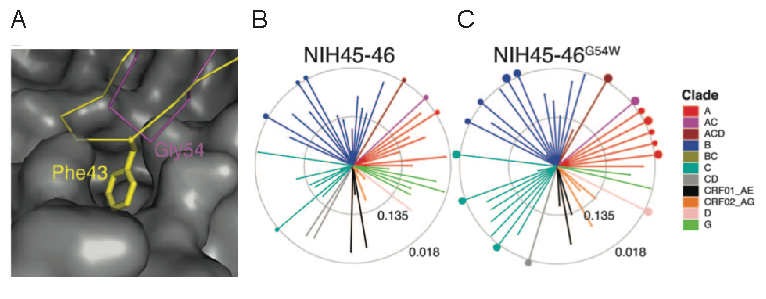
\includegraphics{images/chapter4/figure4_1.pdf} % requires the graphicx package
   \caption[Rational Design of NIH45-46 to Increase Neutralization Potency]{Rational design of NIH45-46 to increase neutralization potency. The gp120 bridging sheet is shown as a surface representation with CD4 shown in yellow and NIH45-46 shown in purple (A). Spider plots showing the neutralization profile for NIH45-46 and point mutant NIH45-46G54W are shown. The length of the line corresponds inversely with the \ic value. Each circle represents a ten-fold change in \ic (B,C). Figure adapted from \citep{Diskin:2011hl}}
   \label{fig:figure4_1}
\end{figure}

\section{Mapping the Energy Landscape of PG9}
\label{sec:mapping}
I retrieved the atomic resolution structure of the complex of mAb PG9 with the CAP45.2.00.G3 variant V1/V2 scaffold from the Protein Data Bank (PDB ID:3U4E) \citep{McLellan:2011dg}. A large number of naturally-occurring 30-amino-acid (30-aa) length HCDR3 antibody sequences was identified in antibody gene repertoires from high-throughput sequencing of antibody amplicons from RNA of B-cells of HIV-negative donors. Retrieval of this dataset is discussed at great length in chapter \ref{chap:chapter3}. A heat map of amino acid occurrences is displayed in figure \ref{fig:figure4_2}A for 30-length HCDR3s. Diversity among the repertoires is seen for all positions 98-118. The sequence conservation at the 5' and 3' ends of the HCDR3 sequences, 96-98 and 118-125, respectively, are due to the ARD motif that make up the 5' end of a canonical neck of a long HCDR3 loop or the J\textsubscript{H}6 template sequence which is seen in a majority of long HCDR3 sequences \citep{North:2011dv,Briney:2012ib}. Between these two stretches of sequences conservation, I observed large sequence diversity. Glycine, tyrosine and serine are generally tolerated at all positions, while proline, lysine and methionine are found less frequently between positions 99-117 (figure \ref{fig:figure4_2}A). This phenomenon is well established in loop unstructured regions connecting beta-sheets in antibodies \citep{Minuchehr:2005wc,De:2005in}.  This propensity for a diverse set of amino acid sequences was the focus of the current study. The idea that there is tremendous sequence space to be explored in 30-length HCDR3s that may further enhance breadth and specificity.

My methods are described fully in the appendix \ref{sec:appendixIII}, but uses the same general protocol as described in chapter \ref{chap:chapter3}. I used the software suite \rosetta to determine the ability of diverse 30-AA HCDR3 sequences to tolerate the structure of the hammerhead configuration of the HCDR3 of PG9 by threading 4,000 naturally occurring unique sequences over the PG9 HCDR3 structure. Once the sequences are threaded, I score them by evaluating the \rosetta scoring function for each position. The contribution to the total score of each position (the sum of all scoring terms of \rosetta), which can be thought of as thermal stability, and the contribution to the binding energy (the total score in complex subtracted from the total score in a separated interface) of each position are evaluated. These are best viewed as heat maps (figure \ref{fig:figure4_2}B,C). These two metrics, total score and binding energy, can be summed to what I define as the mutational "fitness". In this way, I can trim the tremendous sequence space as viewed in the heat map in figure \ref{fig:figure4_2}A, to a focused sequence space to mutations that advantageously effect either thermal stability or binding energy like in the heat maps of figure \ref{fig:figure4_2}A-B, an advantage to using structure based metrics in exploring design. As expected, PG9 itself scored as the most fit sequence for a majority of amino acid positions for the HCDR3 (dots plotted in figure \ref{fig:figure4_2}).

\begin{figure}
   \centering
   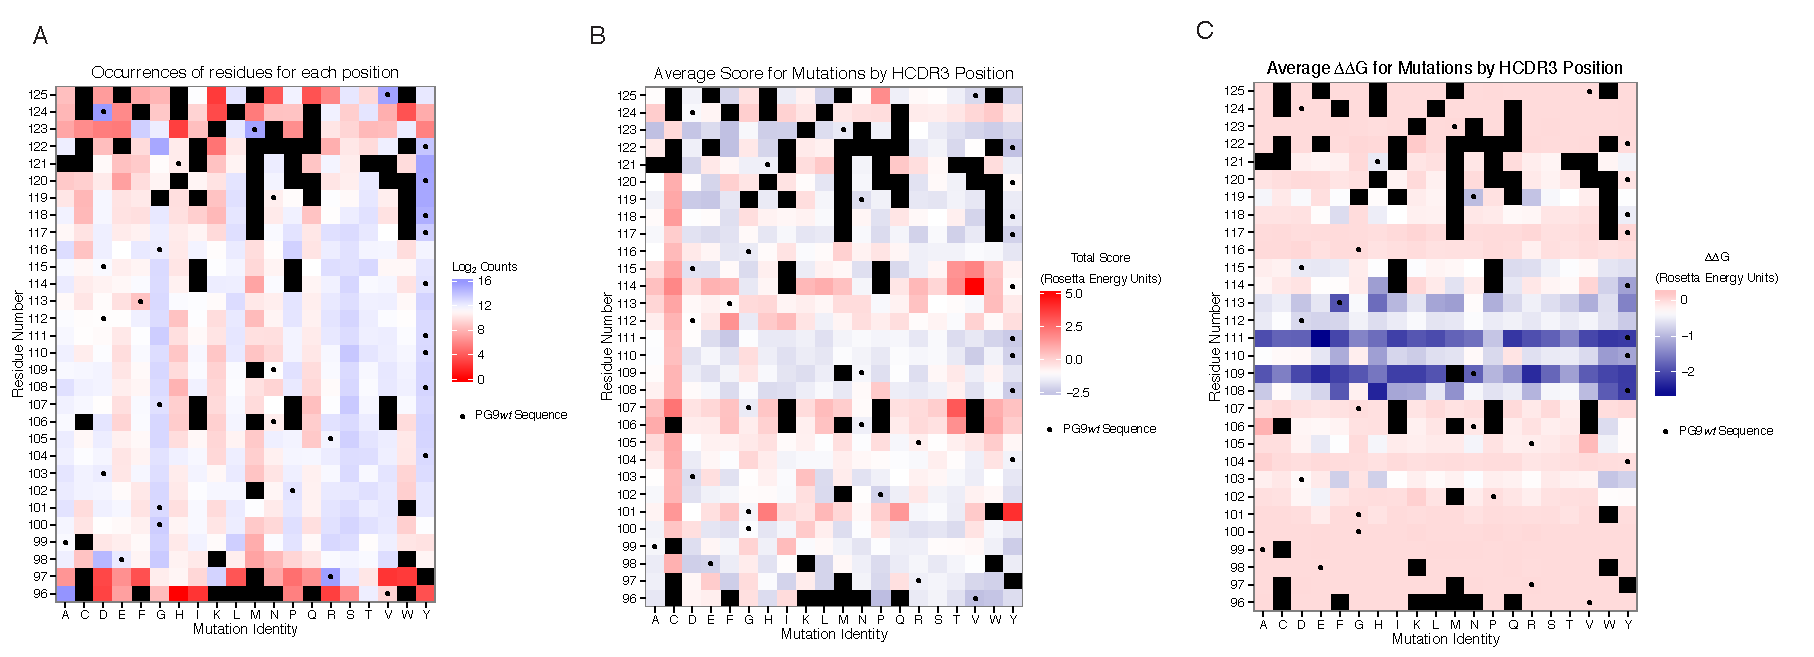
\includegraphics[width=.99\textwidth]{images/chapter4/figure4_2.pdf} % requires the graphicx package
   \caption[Amino Acid Usage and Energy Landscape of PG9]{Amino Acid usage and energy landscape of PG9. Mutation identity is plotted on the x-axis with each of the positions in the 30-length HCDR3 on the y-axis. The usage of each amino acid is shown in a Log\textsubscript{2} blue-red scale counted from 26,422 HCDR3 sequences (A). 4000 random sequences are chosen and their individual score from the \rosetta energy function is shown on a blue-white scale (B).  The same 4000 random sequences contribution to binding energy is shown on a blue-white scale (C). For A-C, the PG9 native sequence is shown as a dot.
}
   \label{fig:figure4_2}
\end{figure}

\section{Redesign of PG9}
Rather than pick the amino acids that had the best fitness for each position, I allowed a complete redesign of the PG9 HCDR3 loop using the \rosettadesign. My reasons for choosing this method rather than a simple matrix lookup generated in the previous section were two fold:
\begin{enumerate}
\item I can account for cooperative mutations. Consider position 99 that has a wild-type alanine for PG9. My heat maps for the energy landscape predict that there are many more favorable mutations I could make including an aspartic acid, asparagine or tyrosine. However, I are unaware if the new mutations are cooperative. That is, do the aspartic acid, asparagine, or tyrosine require neighboring mutations to be fully stable? The complete redesign allows us to account for cooperative mutations while recapitulating the energy landscape predicted in \ref{sec:mapping}.
\item Using a combination of filters and movers based on my specific design goals, I can prevent \rosetta from designing to far away from the original PG9 sequence, position, and structure. I can also tell the \rosetta scoring function to optimize for binding energy, thermal stability, or a combination thereof. This information would be lost on a matrix lookup \citep{Fleishman:2011ji,Kaufmann:2010ea,Kuhlman:2000tc}.
\end{enumerate}

Again, the full design protocol is detailed in the methods section in appendix \ref{sec:appendixIII} and follows the same basic structure as the redesign of sequences detailed in chapter \ref{chap:chapter3}. I designed 1000 decoys allowing small docking perturbations and minimal backbone movement. I filtered the design to optimize for binding energy. That is, only return sequences if favor the binding energy of the mean binding energy of wild-type PG9.

The easiest way to view the sequences returned from the PG9 redesign is with a sequence logo representation (figure \ref{fig:figure4_3}A). The x-axis is the PG9\textit{wt} sequence while the height of the letters at each position, measured in bit, measure \rosetta's preference for that amino acid given the nature of the design challenge. As expected from the observations from the energy landscape (figure 4.2), the original PG9 sequence was returned for a majority of the positions, considering the evolutionary sequence bias of the PG9 structure (nature optimizes sequences for the PG9 structure).  Regardless, anytime an amino acid was returned in 10\% or more of the models, I further inspected the design fitness of the mutation.

I measure the design fitness as a sum of the difference in total energy from wild-type sequence and the difference in binding energy from the wild-type sequence ($\Delta\Delta$G + total score). For some of the positions, multiple amino acids were recovered rather than the wild-type, for example position 109 (figure \ref{fig:figure4_3}A,B). For most positions, the design fitness was negligible, falling above the noise threshold (dashed line) in figure 4.3B. However design at antibody amino acid positions 104, 109, 115, 120, and 123 (PDB numbering) returned alternative amino acids that were predicted to increase HCDR3 fitness for the antibody/HIV-V1/V2 interaction (figure \ref{fig:figure4_3}B).

I wanted to make sure that each of these mutations made intuitive sense upon examination of the structure. I viewed each mutation in context and compared it to the wild-type amino acid. My aim was to determine if this mutation was an artifact and to confirm that it was non-cooperative with other mutations, that is, the mutation enhances fitness alone and not in cooperation with many other mutations made to the sequence. This is because I wanted to retain as much of the PG9\textit{wt} sequence as possible. These visual inspections are shown in Figure 4.3B in the table, with a full justification given. If a mutation was found to be non-cooperative, and still enhance fitness, it was immediately considered for experimental characterization (green squares), N109Y and D115N met these criteria. I also considered N109L and a cooperative mutation A99S and Y120N as they showed strong stabilization through inter-HCDR3 loop hydrogen bonding. I also made one combinatorial mutation that included the double cooperative mutant A99S-Y120N and two single mutations D115N and N109L. This variant is simply referred to as PG9\_4MUT (figure \ref{fig:figure4_3}C). I did not pursue further evaluation of designs that appeared to compromise the structural integrity of the HCDR3 loop.

\begin{figure}[!t]
   \centering
   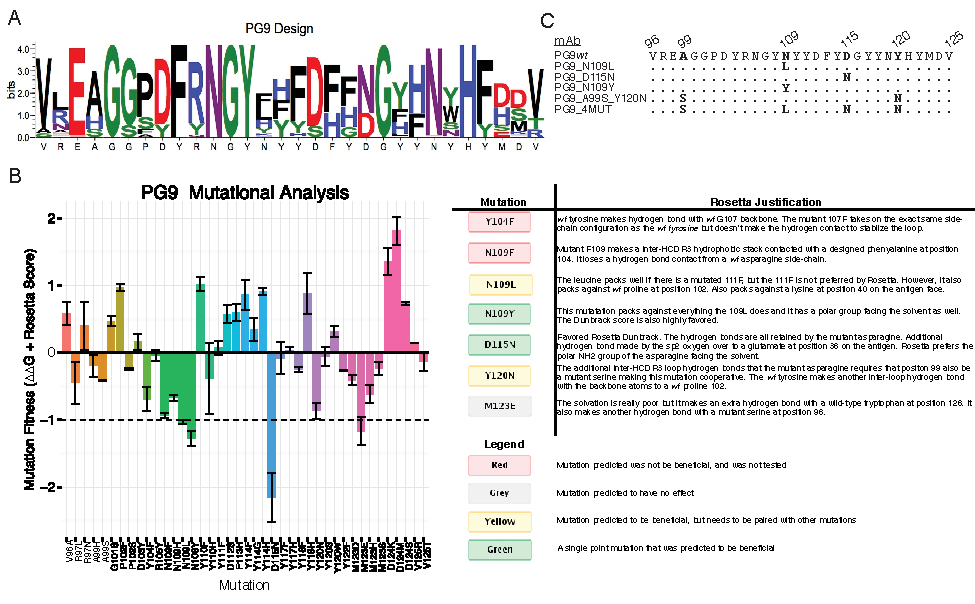
\includegraphics[scale=1.5,width=.99\textwidth]{images/chapter4/figure4_3.pdf} % requires the graphicx package
   \caption[Redesign of PG9 HCDR3]{For 1000 designed models, the sequences returned are best viewed as a sequence logo. The x-axis is the PG9wt sequence while the y-axis represents the preference, measured in bit, of the amino acid identities identified by the height of the letter (A). For sequences that were returned greater than 10\% of the time, I manually inspected their fitness as a measure of binding energy and thermal stability (y-axis). Some positions had more than one amino acid favored and are grouped by color. \rosetta noise is plotted as a dashed line at -1. The more negative a mutation is, the more it is beneficial to the PG9 complex. Each mutation is visually inspected and justified (table). They are either a single point mutations that benefits, a cooperative mutation that benefits, no benefit or detriment, and detriment to the complex, as green, yellow, grey, and red, respectively (B). The final mutations that are chosen to be carried out experimentally are three point mutations and two combinations thereof (C).}
   \label{fig:figure4_3}
\end{figure}


\section{Experimental Characterization of PG9 Variants}
For the five mutational variants of PG9, I used a similar cloning strategy as described in chapter \ref{chap:chapter3} that takes advantage of unique cloning sites between the HCDR3 5' and 3' ends. Each of the variants expressed well. I began by testing all the variants against a 15 antigen mix of gp120 envelopes to qualitatively measure binding. In this preliminary study, the double mutant, A98S-Y120N produced a significantly lower signal than that of PG9, and this variant was not considered further.

PG9\textit{wt} does bind to some gp120 monomers (although PG9\textit{wt} also can neutralize HIV variants for which it does not bind to monomer). I used a panel of representative gp120 monomers from HIV clades B and C to perform screening for binding of PG9 variants to Env \citep{Li:2006kv,Li:2005go}. The results were in good agreement with previous studies of the binding of PG9\textit{wt} to gp120 monomers \citep{McLellan:2011dg}. For these PG9 variants, I calculated half-maximal effective concentration (\ec) values. For each gp120 monomer tested, the PG9 variants N109L and N109Y exhibited 2.3-14.2 fold stronger binding than did PG9\textit{wt} (figure \ref{fig:figure4_4}), while PG9 variant D115N exhibited comparable binding energies to PG9\textit{wt}. PG9\_4MUT exhibited 2-100 fold reduced binding. This is most likely due to the A98S-Y120N mutation that I had previously determined as deleterious.

I also determined the \ec for binding of these PG9 variants to a recombinant form of native gp140 trimer that is recognized by PG9, termed BG505-SOSIP.66419-21. In these assays, both PG9 variants N109L and N109Y exhibited 3.5- or 5.9-fold stronger binding respectively than PG9\textit{wt}. In addition to the stronger binding affinity, the variant N109Y bound to trimer with a complete sinusoidal curve and a strong maximum signal mimicking the binding profile of the glycan-specific mAb 2G12, which is optimal for binding to the trimer \citep{Sanders:2013gm}  (figure \ref{fig:figure4_4}A). The extreme change in maximal signal is intriguing, and may suggest changes in valency of P9 to the trimer \citep{Julien:2013jp}.

I next tested the panel of redesigned PG9 variants and PG9\textit{wt} for neutralizing activity against a panel of viruses displaying PG9-susceptible or -resistant HIV Env molecules, using a TZM-bl neutralization assay \citep{Montefiori:2009hj}. The PG9 variant N109Y exhibited increased neutralization potency for all viruses tested, including viral variants for which PG9\textit{wt} did not have activity (i.e., had neutralization concentration >33 \mcml) (figure \ref{fig:figure4_4}B). Remarkably, PG9 variant N109Y neutralized at 3.72 \mcml~an HIV strain with the N160A mutation that removes the glycan at that position that is required for binding of PG9\textit{wt}6. The PG9 variant N109L also exhibited an increase in potency against HIV strains compared to PG9\textit{wt}, although not at the same level as the PG9 variant N109Y. For all assays tested, N109Y and N109L consistently had enhanced breadth and potency.


\begin{figure}[!t]
   \centering
   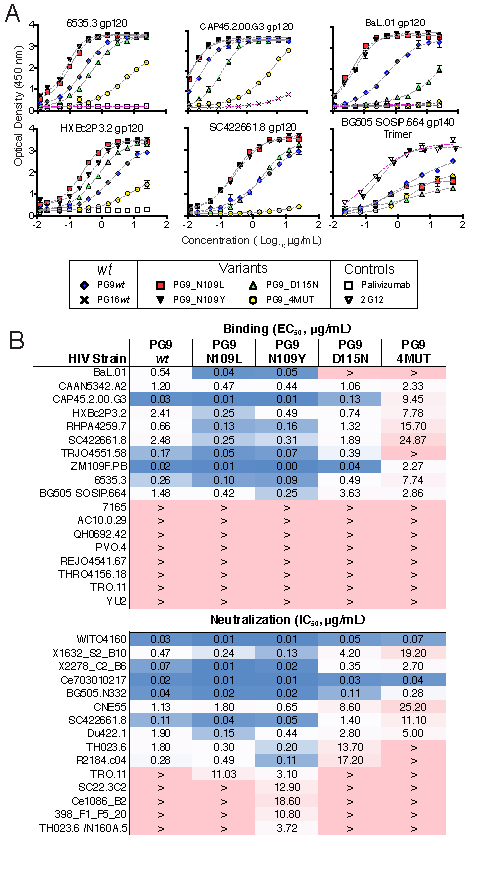
\includegraphics{images/chapter4/figure4_4.pdf} % requires the graphicx package
   \caption[Experimental Analysis of PG9 Variants]{Representative binding curves are shown with the optical density at 450 nm shown on the y-axis plotted against the log\textsubscript{10} concentration in \mcml~on the x-axis (A). All \ec values are calculated from the curves like the ones shown in (A) as well as the neutralization \ic~against a 15 virus panel (B)}
   \label{fig:figure4_4}
\end{figure}


\section{Models to Corroborate Experimental Outcome}
I sought to develop a predictive model to determine the molecular basis for the increased potency and breadth of these PG9 variants using the \rosetta scoring function. I generated three different mutants D115N, N109L and N109Y, which were compared to that of PG9\textit{wt} using the \rosetta scoring function (figure \ref{fig:figure4_5}A). I analyzed the top 25 models for each of the scoring metrics shown. my scoring metrics were binding contribution for the HCDR3, binding for the full complex, total score for the bound and unbound structure ($\Delta\Delta$G). For each metric calculated, I observed statistically significant improvements in HCDR3 stabilization for N109L or N109Y (p < 0.01 or p < 0.001, respectively), but none of my other metrics.

Upon examination of the predicted structures of the top scoring models, I found the antibody position 109 was located on an antiparallel $/Beta$-sheet at the apical tip of the HCDR3 forming a hydrophobic pocket near the interface of the antigen and apical tip (figure 4.5B). The pocket is formed by antibody residues Y104, Y110 and P102 of the antibody heavy chain (PDB numbering). In addition, D167 on the antigen face makes contact with this position. Examination of the structure revealed that the bulk of the hydrophobic amino acid at this position of the pocket contributes to stabilization of the preferred structure of HCDR3. The small hydrophobic bulk of the asparagine fills the pocket, but as the bulk increased to a leucine and then a tyrosine, the predictive model suggested a further stabilization of the HCDR3 loop. In addition, the polar group on the end of the designed tyrosine at position 109 points into solvent space, recapitulating the effect of the polar head of the original asparagine PG9\textit{wt}t.

It is important to note that since I calculate the stabilization as the total energy of the HCDR3 loop, it can be dissected into the individual scoring terms given by \rosetta. These are both described in the chapters \ref{chap:chapter1} and the appendix \ref{chap:appendix}. I have broken the total score down for the HCDR3 loop in figure \ref{fig:figure4_6}. There is little deviation for most of the scoring terms, however, both the attractive force term, the solvation term are improved for the N109L and N109Y mutations. In addition the N109Y shows a favored $\pi$-$\pi$ term. These interactions are accounted for in the model as the N109 position is between a large hydrophobic bulk. In addition, position N109Y also achieves a more favorable $\pi$-$\pi$ stacking interaction with residue Y110 compared to PG9\textit{wt} as the aromatic ring of the designed tyrosine can stack with position 110.

\begin{figure}[!t]
   \centering
   \includegraphics[width=.99\textwidth]{images/chapter4/figure4_5.pdf} % requires the graphicx package
   \caption[Predictive Models of PG9 Variants that Enhanced Binding]{The top 25 models for each binding metric are analyzed. The x-axis is each of the variants and the y-axis is the \rosetta energy units. The metrics are decomposed by binding energy (A) and thermal stabilization (B). Just the HCDR3 is considered (left) or the entire complex (right). Surface representation of position 109. Green is the antigen labeled V1/V2, blue is the HCDR3 loop, dark green is the N160 glycan. Each mutation of interest is shown as a sphere representation that is adjusted to fit the \rosetta atom radius. Spheres are colored by atom type with oxygen in red, nitrogen blue, and carbon in grey. Hydrogens are removed for clarity.}
   \label{fig:figure4_5}
\end{figure}


\begin{figure}[!t]
   \centering
   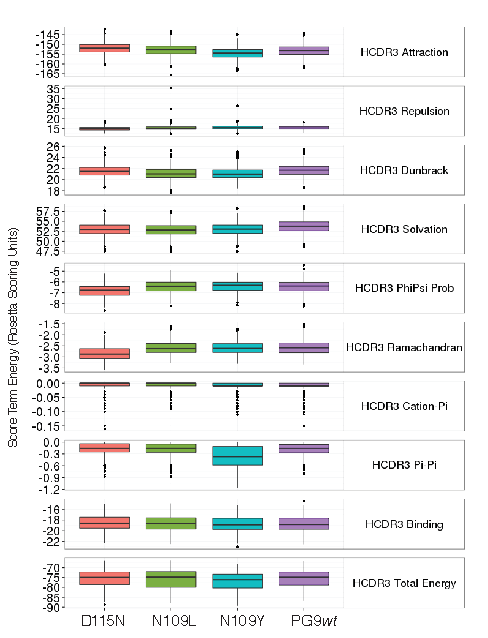
\includegraphics[scale=1.4]{images/chapter4/figure4_6.pdf} % requires the graphicx package
   \caption[Decomposed Scoring Terms for PG9 Variants]{Decomposed scoring terms for PG9 variants. The contribution of individual scoring terms to the total energy score for the HCDR3 loop for each mutation. The predictive model used 1000 simulations for each variant. Each scoring term for \rosetta is shown in the y-axis panel. The y-axis value is the score for that energy term.}
   \label{fig:figure4_6}
\end{figure}


\section{Discussion}
These results have important implications for antibody and vaccine design. The studies reveal the power of \rosetta computational modeling to design antibodies with improved function using structural predictions. Remarkably, the improvements in neutralizing potency and breadth observed here for PG9 variants were achieved not by altering interface residues, but rather by increased thermodynamic stability of HCDR3 loops discovered using a holistic model to determine stability of an antigen-antibody complex. This finding is consistent with recent mutagenesis experiments showing that non-contact residues are essential for antigen recognition by many broadly neutralizing antibodies to HIV \citep{Klein:2013iz}. Non-contact residues in antibody frameworks contribute to high affinity binding by facilitating formation and stability of a pre-configured, low energy binding site \citep{Willis:2013dd,Manivel:2000wk,Marlow:2010jl,Wedemayer:1997wn,Schmidt:2013ka}. Optimally configured binding sites form ordered paratopes that pay a smaller entropic penalty upon forming antibody-antigen complexes \citep{Marlow:2010jl}.

This work shows the efficiency of combining \rosettadesign computational experiments with expert knowledge and wet laboratory validation experiments. For a HCDR3 loop of 30-AAlength, 600 single point mutants are possible, and the number of variants with more than one mutation is enormous. From this large potential set of mutated antibodies, \rosettadesign identified a focused panel of candidate PG9 variants, from which a small subset was considered favorable, and two of five experimentally tested variants exhibited enhanced potency and breadth of neutralization. The computational experiments provided tremendous enrichment for variants with improved binding, but as expected was not completely accurate. For example, although the predictive model suggested that D115N would have the greatest increase in fitness (figure 4.3) this variant was not improved in activity.
The negative result is important, as \rosetta often predicts design failures, and their exploration is fundamental in improving the \rosetta algorithm and scoring function for the most accurate representations of experimental observation. This computational-experimental feedback has been instrumental to my work and will be the target of my future directions.

With the combination of high-throughput sequencing, rapid threading, and experimental feedback, I complete a robust bioinformatics pipeline that can rapidly test antibodies for improvement based solely on their \silico predictions. The results here suggest that there probably is a diversity of antibodies with long and structured HCDR3s that fit the PG9 topology in nature with HIV neutralizing activity that have yet-to-be discovered. I hypothesize this conclusion from three parts of evidence:
\begin{enumerate}
\item Examination of the energy landscape of PG9 suggests that there are mutations which are predicted to be better suited for the PG9 topology.
\item PG9 and PG16 diverge in sequence but converge on a structural topology and have approximately identical specificities and potencies \citep{McLellan:2011dg,Pejchal:2010fp,Pancera:2010hh}.
\item I have discovered point mutations in PG9 that enhance breadth and specificity.
\end{enumerate}
These yet to be discovered antibodies may possess higher HIV inhibitory activity and breadth than the antibodies that are currently in hand. Additional antibody exploration efforts may be worthwhile to identify antibodies of interest with which to design epitope mimetic vaccines, as has been successfully recently implemented \citep{Correia:2014jp,Jardine:2013hb}.



\section{Conclusions and Future Directions}
Two observations may be critical to explore in this current work. It almost seems benign, but the maximum signal difference in the binding assay for the BG505-SOSIP trimer between my variants and the PG9\textit{wt} is worth further exploration. Julien and colleagues observed that PG9 recognizes the trimer asymmetrically \citep{Julien:2013jp}. There are three epitopes displayed on the apical tip of the gp120 trimer, yet PG9 only has a 1:3 valence. The molecular mechanism for this trimeric preference is unavailable due to the high resolution of the structure reported in the study, but the model suggests that PG9 may interact with adjacent N160 glycan. Could the mutation cause a change in valence? This would explain to the maximal signal change in my binding assay. Future experiments could replicate the study performed by Julien et al. either with high-resolution gel-filtration or isothermal titration calorimetry.
Another observation is the glycan independence of the N109Y variant. It was originally thought that any V2/V3 binder would have a dependence on glycans at position N160 and N156/N1706 considering they not only block the recessed C-strand epitope, but make considerable binding contributions to both PG16 and PG9 \citep{McLellan:2011dg,Pancera:2013ev}. It was demonstrated that these glycans are needed for recognition and specificity as mutational experiments completely abrogated neutralization. I are able to replicate that finding, however, my variants can still neutralize glycan knockout variants, albeit, at much lower potency (3.52 \mcml). It is worth replicating this "glycan independence" with many more viral species that have been mutagenized to knockout glycans. I have already begun to pursue this aim.

Finally, I can transpose this entire technology to PG9's sibling, PG16. I already have the mutational candidates ready, and they are being synthesized at the time of this publication. It is important to keep in mind that PG16 specific to the trimeric Env, so it can only be tested with neutralization experiments or if I synthesize stable trimer \citep{Sanders:2013gm}.





\chapter{Conclusions and Future Directions}
\label{chap:chapter5}
\section{Chapter \ref{chap:chapter2} - Multi-state design and polyspecificity}
I expound on the limitations of \rosettadesign by looking at the imperfect agreement between what we expect \rosettadesign to recovery and what was actually observed. I bin these into three categories, Mature sequence bias, evolutionary sequence bias, and incomplete ensemble bias. Section \ref{sec:maturebias} accounts for mature sequence bias, which may be the most difficult to expand understand. When a residue is ``important'' for most of the antibody-antigen complexes, it should be recovered often. However if it only is important in a few complexes, then any given residue can meet the design challenges for the complexes in which it is not important.

Section \ref{sec:evobias} refers to evolutionary sequence bias. Here we may see imperfect agreement with the design and actual antibody sequence simply because the antibody has not achieved maximal potency. \rosettadesign may have selected better amino acid sequences for the epitope. Give enough time to for complete antibody evolution, the sequence may have matched. This is founded on the principle that \rosettadesign gives the best sequence for any design challenge.

Section \ref{sec:limits} gives the limits of computation including the finite ensemble size that states there are not enough PDBs to compensate for ``structural space'' that \rosettadesign samples. This section also details some of the more classic limitations including the limits of the \rosetta scoring function and limitations of the sampling algorithms. In the future this may be ameliorated with more structures being deposited to the PDB, and improvements to the scoring function including explicit solvent modeling.

The power of chapter \ref{chap:chapter2} is in the future directions. While we use multi-state design to interrogate the flexibility of the germline repertoire, the end goal was always to design cross-binding antibodies. Many pathogens which evade traditional vaccination do so by evolving multiple serotypes or antigenic variants that encompass a tremendous sequence space. HIV, Influenza and Dengue virus (DENV) are such examples of antibodies which use antigenic variation as a means to evade a broadly protective immunogenic response. It is to these pathogens that a broad cross-reactive response will be critical \citep{Corti:2013ex,Lanzavecchia:2009dd,Corti:2011ku,Simonelli:2013jc}. Multi-state design will be invaluable in the design of these antibodies. Consider \ref{fig:fig5_1}, here we take a known cross-reactive group 1 antibody against influenza known as CR6261 \citep{Throsby:2008dc} which does not bind to Influenza type B.

\begin{figure}[!t]
   \centering
   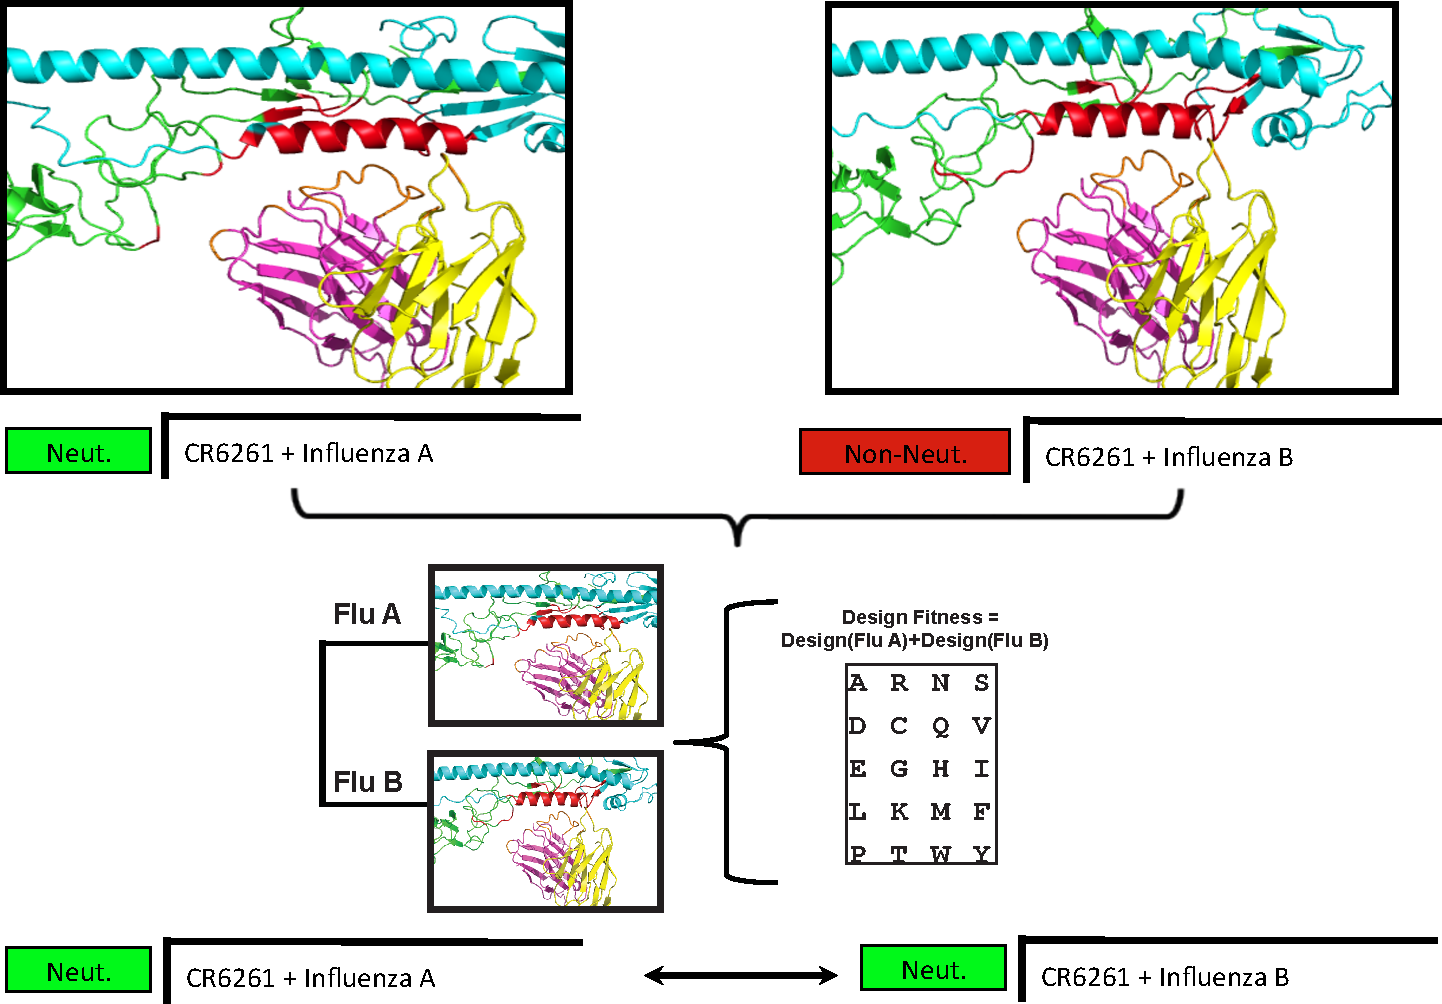
\includegraphics[width=.9\textwidth]{images/chapter5/figure5_1.pdf}
   \caption[Multi-state Design of Broadly Neutralizing Influenza Antibodies]{Multi-state design of broadly neutralizing influenza antibodies. Initially, the antibody CR6261 only binds and neutralizes only Influenza A subtypes. Using multi-state design I plan to make minimal mutations at the interface that allow binding to Influenza type B while retaining binding to Influenza type A. This principle allows me to design in cross-specificity.}
       \label{fig:fig5_1}
\end{figure}


I even took this idea into the lab looking at special cases for influenza antibody. I considered the antibody CR6261 as it was bound to the stem portion of influenza \citep{Corti:2011ku}. At the stem region, their is less conformational diversity. I hypothesized that this epitope loses neutralization affinity due to point mutations at the interface rather than large conformational shifts that are evident in the head region. This would be easier for \rosettadesign to recover. First I wanted to create a proof-of-concept by seeing if we can enhance specificity to already known binders. I choose H1/South Carolina/1918 and H5/Vietnam/2004 pandemic strains as both had a crystal structure to CR6261. Using multi-state design, I told \rosettadesign to enhance binding to both variants. Figure \ref{fig:fig5_2} shows the design process. The sequence logo in (A) shows the amino acids preferred at the interface. For (B), we analyzed the fitness of each mutation as either having beneficial or deleterious effects. If it enhanced fitness for both H1 and H5, we made the mutations in the laboratory. They indeed did enhance binding to both variants compared to wild-type CR6261 (figure \ref{fig:fig5_2} C.).

\begin{figure}[!t]
   \centering
   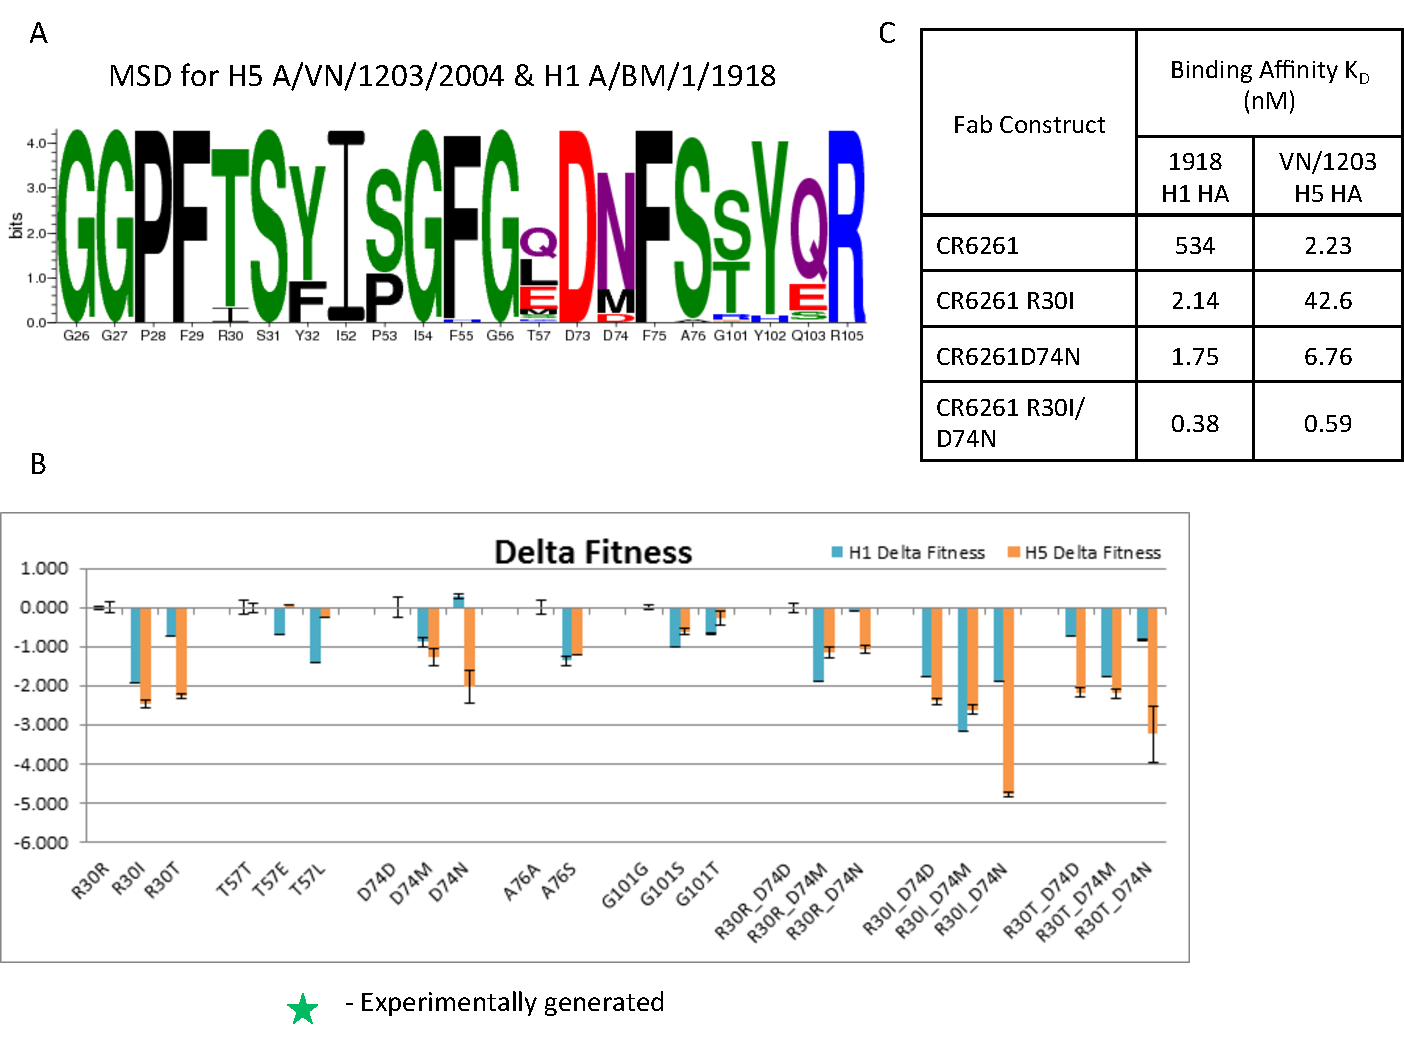
\includegraphics[width=.9\textwidth]{images/chapter5/figure5_2.pdf}
   \caption[Preliminary for MSD Proof-of-Concept]{Preliminary for MSD proof-of-concept. A sequence logo for all positions considered for redesign at the interface. Higher letters indicate \rosetta's proclivity for a certain amino acid sequence (A). Fitness analysis of each position is a sum of stability and binding energy. Lower energies indicate better fitness. Ideally, both H1 and H5 would have decreased fitness energy. Stars indicate mutations that were made experimentally (B). The binding affinities from the suggested mutations from \rosetta. The double mutant gives the best binding affinity (C).}
       \label{fig:fig5_2}
\end{figure}

Of course this mild proof of concept can extend well beyond Influenza. My plan was to use this to get a serotype specific antibody to bind (and therefore, potentially neutralize) cross-serotype, cross-group, and cross Influenza type. However, many groups are trying to design cross specific antibodies. One advantage of multi-state design is that if you fine-tune specificity you do not have to lose specificity to your original epitope. For example, in a paper by Simonelli \textit{et al.} \citep{Simonelli:2013jc}, they used computational modeling along with NMR restraints to place give a molecular definition of an anti-DENV against all four DENV serotypes. They then used their knowledge of rationale design to fine tune specificity to each serotype individually. However, upon making one mutation specific to a given serotype often abrogated binding to the others. Therefore it is possible to enhance breadth at the cost of specificity. This type of problem is ideal for multi-state design as it can fine tune specificity without predicted loss of binding to your original epitope.

In related work, structural viral homologs could also be used in multi-state design. For example, an antibody found in chronically exposed repository infected patients bound and neutralized four different paramyxoviruses, human respiratory syncytial virus (HRSV), human metapneumovirus (HMPV), bovine RSV (BRSV) and pneumonia virus of mice (PVM) \citep{Corti:2013cv}. This antibody was found by screening a common structural homolog (prefusion protein F) against anti-HRSV screened from over 200 donors to narrow down their search. I hypothesize that this type of structural information can be used in multi-state design to make \textit{de novo} designed cross-neutralizers much the way nature selected cross-neutralizers from these patients.

Finally, there is much use for this algorithms fitness function. While I describe antibody design in the context of \textit{designing for} a certain antigen, it may be beneficial to \textit{design against}. I can modify the scoring function in such a way where we select mutations that will \textit{design for} one antigen, and \textit{design against} others. This allows any fine tuning of specificity changes that are needed against antibodies while not compromising the structural integrity of the immunoglobulin fold. I can imagine this will be an invaluable tool for designing against antigens that are found to be related to autoimmunity.

\section{Chapter \ref{chap:chapter3} - Broadly neutralizing antibodies from HIV-\naive repertoires}
In chapter \ref{chap:chapter3}, I used antibody design to interrogate the HIV-\naive repertoire to answer a simple question for the paradigms of HIV vaccinology. How close is the \naive repertoire to eliciting neutralizing antibodies. I used the principles guided by both reverse  and forward vaccinology\citep{Burton:2012bh}. Reverse vaccinology principles require that the broadly neutralizing antibodies are first characterized from chronically infected patients. I used the the V1/V2 binding antibody PG9 that was discovered in a chronically infected African donor \citep{McLellan:2011dg,Walker:2009cd}. This is were I introduced a new paradigm into vaccinology. Rather than used structure based immunogen design from the PG9 epitope which has been characterized, I instead investigated the healthy donor repertoire. In my early work here, I had helped discover long HCDR3s in healthy donors, and it was with this information I wanted to pursue this question.

I conclude that although there are some antibodies from the HIV-\naive repertoire that are able to mimic PG9 hammerhead like configuration, there are very few from our population pool. Even those that we did find needed some amounts of mutation that honed specificity to make these antibodies truely binding and neutralizing.

There is an absolute limitation to this study, and that is the amount of long-HCDR3 sequences we started with. Out of one-half-billion sequences, we only were able to obtain ~26,000 unique 30-length sequences that were viable in our study. That is an incredibly low amount. Along with Andy Fire, Jessica Finn and myself, we have deviced new clever experiments that can potentially enrich for long HCDR3s. We have noticed that in this study and previous studies, that most antibodies with long HCDR3s contain a J\textsubscript{H}6 gene segment \citep{Briney:2012ib}, in addition, PG-type antibodies often use V\textsubscript{H}3-30 genes. This makes the initial PCR rounds for gene-specific targeting a simple task. Rather than use ambiguous primer-sets for all gene families, I plan to use just specific primers to J\textsubscript{H}6 and V\textsubscript{H}3-30 for amplification of B-cell mRNA transcripts. I can actually predict that this will enhance the mean HCDR3 length from 15.56 to 18.06 (figure \ref{fig:fig5_3}). In addition, new advances in high resolution gel electrophoresis allow single base pair resolution and purification. That would allow only very-long HCDR3 sequences to be purified and enriched from the canonical length background. Using this, I could truly use this population pool in my newly created bioinformatics pipeline to test the HIV-\naive donor sequences.

\begin{figure}[!t]
   \centering
   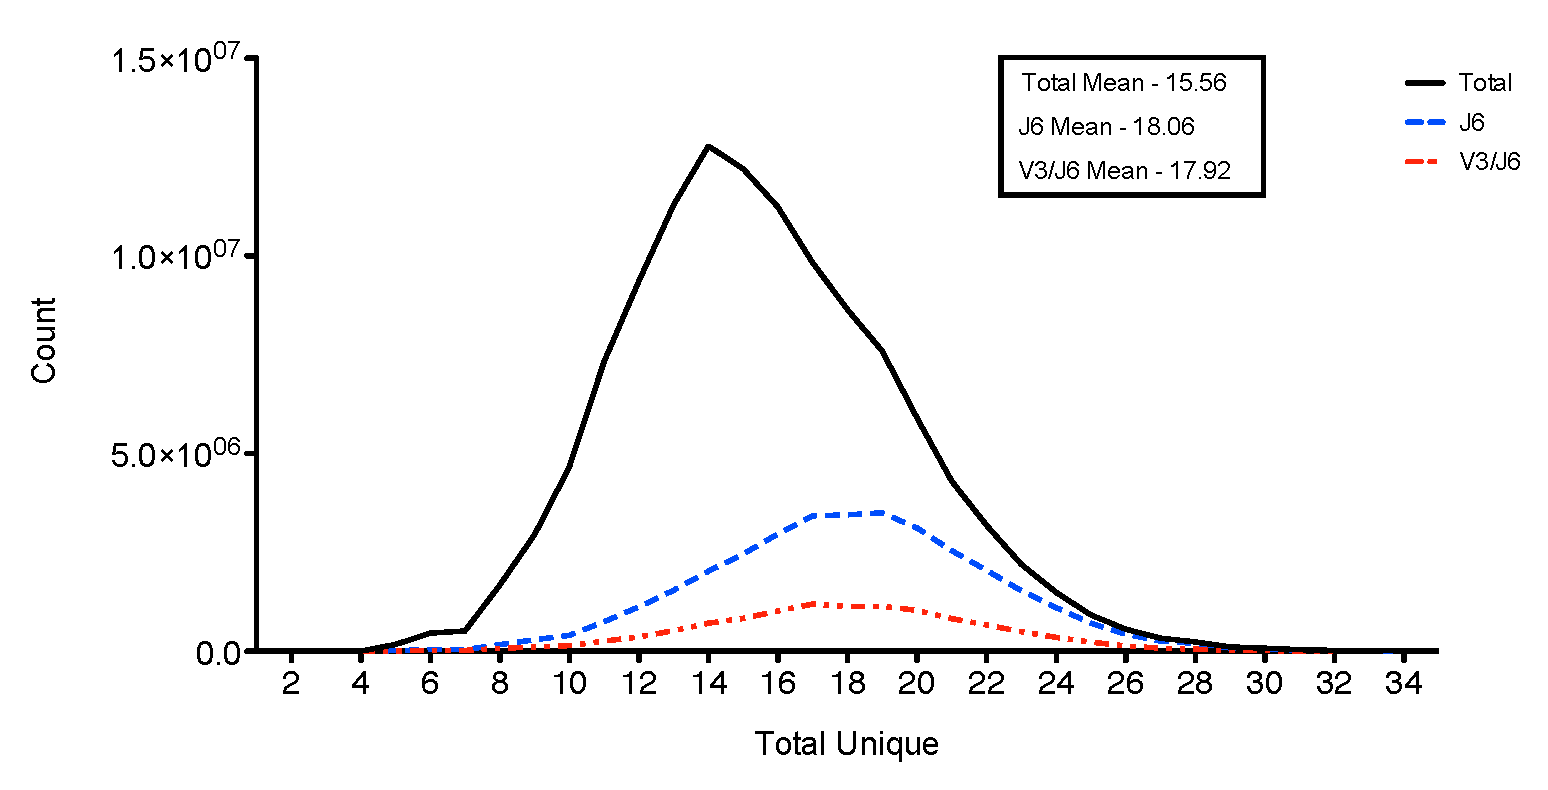
\includegraphics[width=.9\textwidth]{images/chapter5/figure5_3.pdf}
   \caption[HCDR3 of J\textsubscript{H}6 Gene Families]{HCDR3 of J\textsubscript{H}6 gene families. A distribution curve for HCDR3 sequences is shown for all VDJ familes (black). When only J\textsubscript{H}6 genes are considered, the mean length shifts from 15.56 to 18.06. If only J\textsubscript{H}6 and V\textsubscript{H}3 gene families are considered the mean shifts down to 17.92.}
       \label{fig:fig5_3}
\end{figure}

One problem that is mentioned is the potential framework bias. Although it has been demonstrated that the HCDR3 loop is responsible for a majority of the contact and by extension the mechanism of neutralization \citep{Pejchal:2010fp,Pancera:2010hh}, it can't be ruled out that the framework provides some contribution to binding in the LHCDR3 and HCDR2 region \citep{McLellan:2011dg}. However, in recent studies, mutations all the way back to germline have shown that these mutations aren't absolutely necessary necessary to necessitate binding and by extension neutralization \citep{Klein:2013iz}. In chapter \ref{chap:chapter2}, we find at least fifty percent of the the germline framework may be necessary for binding, even those residues that lie extremely distal to the interface. This leads me to believe in an inherent framework bias in our study. I used PG9 framework as the complete sequence to the rest of the heavy chain and the light chain was unknown (the current technology is limited at the time of writing). But other studies show us that surrounding mutations of the HCDR3 loop allow it to form its native conformation \citep{Wong:2011ff}. I want to know the effects of other germline frameworks on HIV-\naive HCDR3 loops.

I proposed a display technology solution to this problem. If I can isolate 30-length (or longer) HCDR3 sequences from the B cell repertoire, I can engineer cloning sites into them as I have done for the PG9 framework. However, each cloning site will be slightly upstream of the HCDR3 site. In this manner we can use any germline framework to test each HIV-\naive conformation. In this way, we can test inherit framework bias from each germline framework on the healthy HCDR3 sequence. For the amount of HCDR3 sequences we get (roughly estimate 100,000 using the technique described above), we can test this on each V\textsubscript{H} gene family, giving 5.2 million different combinations of antibodies we can test and remove framework bias. In addition, we can combine germline light chain repertoires to increase our combinations. I feel like this would be like an incredibly useful experiment to find antibodies from HIV-\naive donors with the absolute minimum amount of mutations. In this way I can get an absolute threshold to describe what a vaccine will need to elicit using a very inexpensive technology.

\section{Chapter \ref{chap:chapter4} - Broadly neutralizing antibody redesign}
I indicate some of the issues with redesign and highlighted them in the publication that accompanies chapter \ref{chap:chapter4}. For instance, \rosettadesign

In figure \ref{fig:fig5_4}, an initial pilot study has been performed.

\begin{figure}[!t]
   \centering
   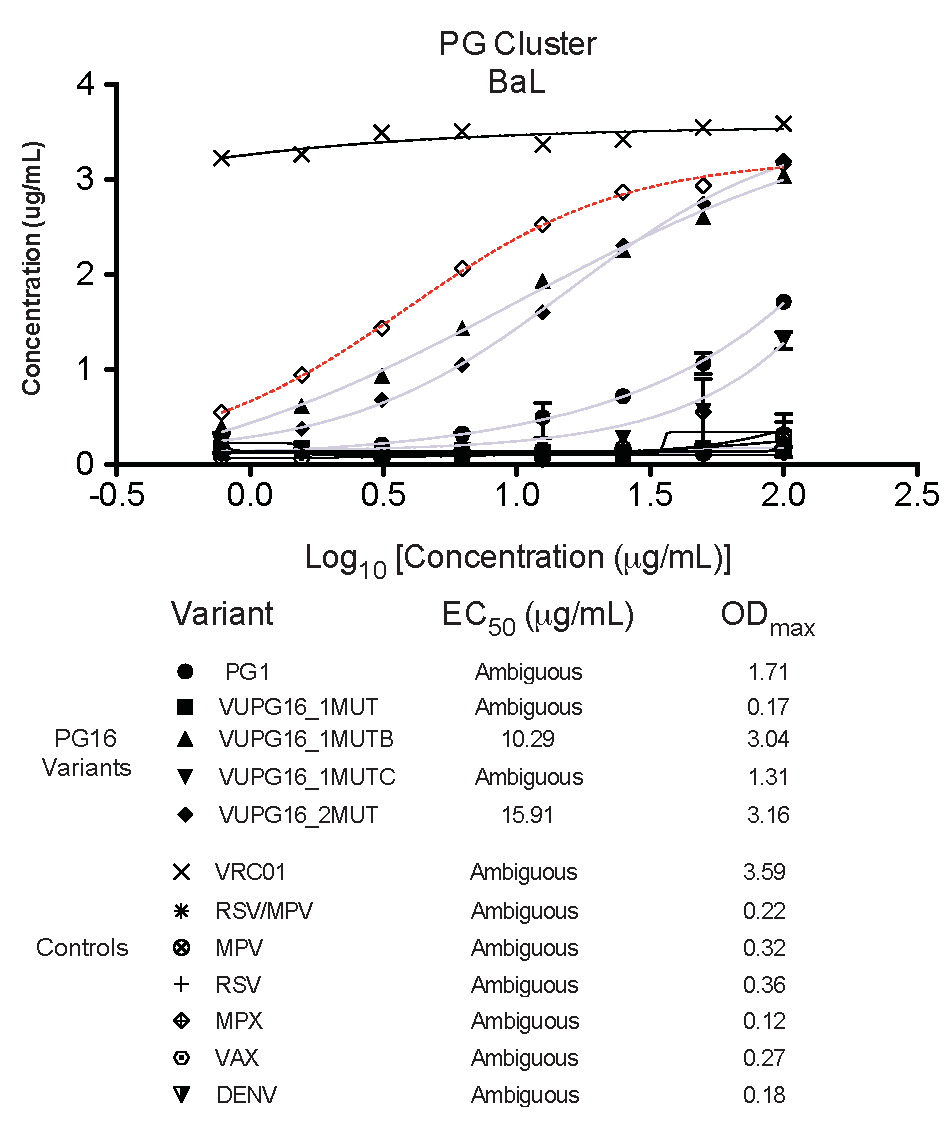
\includegraphics[width=.9\textwidth]{images/chapter5/figure5_4.pdf}
   \caption[Binding Profile of PG16 Variants]{An initial pilot study with PG16 HCDR3 variants on a PG9 backbone. All the variants have a PG9 backbone except for PG16\textit{wt} which may explain the strength in binding. Various negative and positive controls are shown for other viral species.}
    \label{fig:fig5_4}
\end{figure}



%\section{Other applications of antibody design - antigen escape}
\chapter{Appendix}
\label{chap:appendix}
%appendix I
\section{Appendix I - \rosetta~Glossary}
\label{sec:appI}
\singlespace
\setlength{\parindent}{0pt}

\textbf{All-atom} - in the case of sampling, synonymous with fine movements and often including side chain information; also referred to as high-resolution \\ \\

\textbf{Benchmark} - another word for a test of a method, scoring function, algorithm, etc. by comparing results from the method to accepted methods/models \\ \\

\textbf{Binary file} - a file in machine-readable language that can be executed \textit{in silico} \\ \\

\textbf{BioPython} - a set of tools for biological computing written and compatible with Python \\ \\

\textbf{Build} - to compile the source code so it may be used as a program \\ \\

\textbf{Centroid} - in \rosetta~centroid mode, side chains are represented as unified spheres centered at the residues center of mass \\ \\

\textbf{Cluster center} - the geometric center of a cluster, or group, of models \\ \\

\textbf{Clustering} -  grouping models with similar structure together \\ \\

\textbf{Comparative model} - a protein model where the primary sequence from one protein (target) is placed, or threaded, onto the three dimensional coordinates of a protein of known structure (template) \\ \\

\textbf{Cyclic coordinate descent (CCD)} - based on robotics, CCD loop closure is used to build loops in \rosetta by fragment assembly and close loops by decreasing the gap between two termini in three-dimensional space \\ \\

\textbf{\textit{De novo}} - from the sequence; also called \textit{ab initio}, with no experimental guidance \\ \\

\textbf{Directory} - synonymous with a folder, usually contains one or more files or other folders \\ \\

\textbf{Distance matrix} - a matrix containing the pairwise distances for every point in a set of points \\ \\

\textbf{Dunbrack rotamer library} - a set of likely side chain conformations for the twenty canonical amino acids based on protein structures in the Protein Data Bank (PDB) \\ \\

\textbf{Executable} - binary file used to execute the program \\ \\

\textbf{Force field/Scoring function/Energy function/Potential} - often used interchangeably; a means of assessing the energy of the generated models \\ \\

\textbf{Fragment} - in \rosetta~folding and loop building, a set of three-dimensional coordinates corresponding to a given amino acid sequence fragment \\ \\

\textbf{Database} - also called the fragment library, contains all the interchangeable data needed for \rosetta \\ \\

\textbf{Gap} - in sequence alignment, a gap is inserted when the sequences are of low homology; usually appear as a dash (-); the gaps form a sequence alignment correspond to areas where loops are
built during comparative modeling \\ \\

\textbf{GDT/GDT\_TS} - global distance test (total score); a measure of similarity between two protein structures having the same amino acid sequence; the largest set of residues C$\alpha$-atoms in the model structure falling within a defined distance cutoff of their position in the experimental structure \\ \\

\textbf{Gradient-based minimization} - also known as minimization by steepest descent; in this case, a means of energy minimization in which one takes steps proportional to the negative of the gradient of the function (energy) at the current point \\ \\

\textbf{High-resolution} - in the case of sampling, synonymous with fine movements and often including side chain information \\ \\

\textbf{Homology model} - a more specific type of comparative model where the protein sequence of interest (target) is a homolog of the protein of known structure (template) \\ \\

\textbf{Interface delta} - the interface delta score is defined as the contribution to the total score for which the presence of the ligand is responsible \\ \\

\textbf{Kinematic loop closure (KIC)} - robotics-inspired loop closure algorithm which analytically determines all mechanically accessible conformations for torsion angles of a peptide chain using polynomial resultants \\ \\

\textbf{Knowledge-based} - in the case of \rosetta, based on information obtained from structures found in the PDB \\ \\

\textbf{Libraries} - in computing, a collection of code and data (classes and functions) used by a piece of software and is often used in software development \\ \\

\textbf{Ligand} - the part of the structure that binds to a protein to serve some biological purpose \\ \\

\textbf{Low-resolution} - a somewhat subjective term, in the case of sampling, synonymous with coarse movements of the protein and/or ligand backbone and side chains; the individual atoms of low-resolution structures or models cannot be resolved, or observed \\ \\

\textbf{Metropolis criterion} - often combined with the Monte Carlo sampling algorithm; allows for generation of an ensemble that represents a probability distribution \\ \\

\textbf{Model} - in the case of this protocol, a structure generated by \rosetta; sometimes called a decoy \\ \\

\textbf{Monte Carlo sampling} - a randomized and repetitive computational sampling method \\ \\

\textbf{Mover} - a generic class that takes as input a pose and performs some modification on that pose; for example, a mover might take in a pose and rotate every residue \\ \\

\textbf{Namespace} - in computer science, an abstract container holding a logical grouping of unique identifiers or symbols; in \rosetta, examples of namespaces are loops, relax, etc. \\ \\

\textbf{Native-like} - close to the experimentally determined structure; a model that is native-like usually has an RMSD to the experimentally determined structure of < 2\r{A} \\ \\

\textbf{Options file} - often called a flags file; a file containing \rosetta~options that can be passed to a \rosetta~executable after the @ symbol; can be easier to use than passing \rosetta~options over the command line \\ \\

\textbf{Pack/repack} - in \rosetta, side chains are packed/repacked by switching out rotamers and scoring them using the \rosetta~scoring function \\ \\

\textbf{Pose} - in  \rosetta~protocol, a three-dimensional conformation of the ligand, protein, or ligand/protein complex at any given time-point \\ \\

\textbf{Python} - interpreted, object-oriented, high-level programming language \url{http://www.python.org/} \\ \\

\textbf{Relax} - in \rosetta, an iterative protocol of side chain repacking and gradient-based minimization; often referred to as full-atom (or all-atom) refinement \\ \\

\textbf{Robetta}  \rosetta structure prediction server (\url{http://robetta.bakerlab.org/}) freely available to not-for-profit users \\ \\

\textbf{RosettaCommons} - a group of more than twenty labs that develop the \rosetta software suite  \\ \\

\textbf{REU} - arbitrary energy units specific to the \rosetta~scoring function \\ \\

\textbf{RosettaScripts} - also called ``the scripter'' or RosettaXML; an XML-like language that allows for specifying modeling tasks in \rosetta \\ \\

\textbf{Rotamer} - rotational conformer of an amino acid or ligand side chain \\ \\

\textbf{SCons} - a tool for constructing software from its source code \url{http://www.scons.org/} \\ \\

\textbf{Script} - in computer programming, a script is a sequence of instructions that is interpreted or carried out by another program rather than by the computer processor (as a compiled program is) \\ \\

\textbf{Source code} - human-readable files that are the implementation of the program; are written in C++ in \rosetta \\ \\

\textbf{Target} - in comparative, or homology, modeling, the protein for which we are generating a model; the target sequence is the primary sequence of the protein for which we want to make a model \\ \\

\textbf{Template} - in comparative modeling, the protein of known structure on which the target is threaded \\ \\

\textbf{Threading} - placing the primary sequence of one protein (target) on the three-dimensional coordinates of a protein of known structure (template) based on a sequence alignment loop building \\ \\

\textbf{XML} - Extensible Markup Language; in this case, used to write protocols to pass to

\clearpage
\section{Appendix II - \rosetta~Scoring Terms}
%appendix II
\renewcommand{\arraystretch}{1.8}
\begin{table}[ht!]
\begin{tabular}{lp{11cm}}
\textbf{Scoring Term}      & \textbf{Explanation of Scoring Term}                                                                                         \\ \hline
Attraction                 & The Van de Walles scoring term to indicate how much attraction residues have on each other                                   \\
Dunbrack                   & A statistical probability score indicating how often a side-chain configuration has been seen in the protein data bank (PDB) \\
Repulsion                  & The Van De Walles scoring term to indicate how much repulsion residues have on each other                                    \\
Solvation                  & How well are hydrophobics packed away from solvent and hydrophillic groups are facing solvent                                \\
Ramachandran               & A statistical probability of how well $\phi$-$\psi$ angles fit into the Ramachandran plot as a function of secondary-structure     \\
Total                      & A summation of all individual scoring terms to get a total score                                                             \\
\ddg                       & The change in total energy score when residues are moved out of complex                                                      \\
$\phi$-$\psi$ Prob         & A statistical probability score of how well a side-chain configuration has been seen given a $\phi$-$\psi$ angle in the PDB  \\
Cation-$\pi$               & A score encompassing how the configuration of positive cation at the end of a charged reisidues interact with pi orbitals    \\
$\pi$-$\pi$                & A score encompassing how two $\pi$ orbitals interact                                                                            \\
HCDR3 Stabilization        & The total score of residues only found in the HCDR3                                                                          \\
Full Complex Stabilization & The total score of all residues representing a free energy of the model                                                      \\
HCDR3 Binding              & The contribution to \ddg~by residues found in the HCDR3                                                                       \\
Full Complex Binding       & The \ddg~for the entire complex
\end{tabular}
\caption[\rosetta~Scoring Terms]{}
\end{table}
\clearpage
\doublespacing
\section{Appendix III - Materials and Methods}
\label{sec:appendixIII}
\par\vspace{10pt}
\subsection{Chapter \ref{chap:chapter2} - Materials and Methods}
\par\vspace{10pt}
\subsubsection{Selection of Antigen-Antibody Complexes}
Diverse antigen-antibody complexes were collected from the Protein Data Bank (PDB; \url{www.pdb.org}) in which antibodies in different complexes were derived from the same predicted heavy chain variable gene segment. Candidate complexes were queried from the protein databank using the IMGT-3D structural query editor for immune system receptors \citep{Kaas:2004kv}. PDB structures were used as design candidates if they met the following criteria: 1) the antibody was encoded by a V\textsubscript{H}1-69, V\textsubscript{H}3-23, or V\textsubscript{H}5-51 gene segment, 2) the structure contained a human immunoglobulin, and 3) the ligand type was a protein complex. The search yielded 10, 8, or 3 antibody-antigen complexes encoded by the heavy chain variable gene segments V\textsubscript{H}1-69, V\textsubscript{H}3-23, or V\textsubscript{H}5-51, respectively. Nature of the antigen and antibody isotype were not considered in the selection as the 21 complexes represent an exhaustive search of the PDB for these gene-segments. The gene segments were aligned using the ClustalW2 multiple sequence alignment algorithm \citep{Larkin:2007hz}. Each input structure was energetically minimized using the Rosetta scoring function but constrained to PDB input backbone coordinates \citep{Das:2007em}.

\subsubsection{Multi-state Design of Antigen-Antibody Complexes}
Three design experiments were performed, one for each of the three germline segments (V\textsubscript{H}1-69, V\textsubscript{H}3-23, or V\textsubscript{H}5-51) using the multi-state design mode of the Rosetta algorithm and scoring functions. I adapted a generalized multi-state design protocol that was described in detail previously that perform design on multiple antibody-antigen complexes at once \citep{LeaverFay:2011ji}. Briefly, each computational design experiment computed an optimal sequence predicted to define a low-energy structure.  In the multi-state design experiments, an energetic consensus sequence for all of the states was predicted, rather than treating each state as a separate entity. The energy for a given sequence was computed and designated the ``design fitness'' for all states. The corresponding amino acids were derived from the alignment (e.g., heavy chain amino acid 5 on complex A corresponded to heavy chain amino acid 5 on complex B). The details of the multi-state algorithm is described elsewhere \citep{LeaverFay:2011ji}.

\subsubsection{Single-State Design of Antigen-Antibody Complexes}
Single-state design was performed using the \rosetta~multi-state application. The algorithm was altered so that only one complex was considered for each of the 10, 8, or 3 design experiments with V\textsubscript{H}1-69, V\textsubscript{H}3-23, or V\textsubscript{H}5-51 complexes, respectively.

\subsubsection{Design Analysis of Multiple- or Single-State Design}
For each design experiment, 100 independent design trajectories were calculated. Sequence logos then were generated using the Berkley web-logo server (\url{http://weblogo.berkeley.edu/})~\citep{Crooks:2004do}. Information for each sequence logo can be extrapolated as follows extending the work of Schneider \textit{et al.} \citep{Schneider:1990ub}. For each variable position, the probability of seeing each of the 20 naturally encoded amino acids p\textsubscript{i} was computed and compared with the background probability p\textsubscript{b} = 1/20 = 5\%. To quantify the deviation of the observed probability from the background probability I compute the self-information for each of the 20 amino acids as I\textsubscript{i} = p\textsubscript{i} x log\textsubscript{2}(20 x p\textsubscript{i}) in `bit'. If the amino acid occurs as often as expected from the background probability, I\textsubscript{i} is zero. Ii becomes larger if the amino acid is over-represented and approaches 4.32 if p\textsubscript{i} = 100\%. A total bit-score for the sequence design was obtained by summing all individual bit-scores for each amino acid. The bit-scores for the target sequence then were analyzed, and statistics were computed using Prism software version 5.0 (GraphPad Software).  For comparisons between germline sequence and mature sequence within the same design experiment, a Wilcoxon matched pairs test (non-normal, paired t-test) was used to compute the p-value at 99\% confidence level. For comparison between design experiments, a student's paired t-test was used to compute the p-value at 99\% confidence level.

\subsubsection{Amino Acid Environment}
The neighbor vector algorithm quantitatively determines the surface-exposure of a given residue and is described by Durham and colleagues elsewhere \citep{Durham:2009kt}. Briefly, each C$/Beta$ is computed to a vector and each vector is given a score based on the number and orientation of each C$/Beta$ in the proximity. The weight of each neighbor falls of as a function of distance.
For interface scores, the change in neighbor vector was used, where the neighbor vector score of the amino acids in the unbound antibody is subtracted from the neighbor vector scores of the complex. Interface residues would have a large change in neighbors and proportional to the change in neighbor vector score.

\subsubsection{Phi-psi Angle Calculations}
All V\textsubscript{H} framework residues were grouped by complex. For each residue, phi-psi angles and secondary structure classification were determined using DSSP \citep{Kabsch:1983bp}. For each residue position across all complexes considered in design, the standard deviation of the phi-psi angles was calculated if they were included in the beta-sheet framework. A student's t-test was performed between the standard deviations between residue positions that recovered to germline (bit-score > 1), or did not recover to germline (bit-score < 1). For a reference, a deviation for all framework beta-sheet positions was also calculated for all residues even if they were not included in the design protocol.
\clearpage
\subsection{Chapter \ref{chap:chapter3} - Materials and Methods}
\par\vspace{10pt}
\subsubsection{RNA Extraction}
Peripheral blood mononuclear cells were isolated from 64 HIV-uninfected individuals (HIV-\naive) by processing leukoreduction filters as previously described \citep{Weitkamp:2001vm} .Briefly, RC2D leukoreduction filters were obtained from the American Red Cross and were backwashed with 35 mL of sterile PBS with 10mM EDTA. The resulting PBMC suspension was overlaid onto 15 mL of HistoPaque 1077 and centrifuged at 600 RCF for 25 minutes. The buffy coat was removed and washed twice with fresh PBS with 10mM EDTA. Total RNA was isolated from 10 million PBMCs using the RNeasy kit according to the manufacturer's standard operating procedure.

\subsubsection{cDNA Synthesis, PCR Amplification and Purification}
cDNA was synthesized from 100 ng of total RNA and 10 pmol of each RT-PCR Illumina-adapter primers in duplicate 50 \microliter~RT-PCR reactions using the OneStep RT-PCR system. The RT-PCR reactions were performed in a BioRad DNA Engine PTC-0200 thermal cycler running the following protocol: 50\degree C for 30:00, 95\degree C for 15:00, 35 cycles of (94\degree C for 0:45, 58\degree C for 0:45, 72\degree C for 2:00), 72\degree C for 10:00. cDNA synthesis was confirmed on a 1\% E-Gel EX. After which duplicate reactions were pooled. 2 \microliter~of each cDNA sample and 20 pmol of each indexed Illumina-adapter primer were used to template 100 \microliter~PCR amplification reactions in duplicate using the AmpliTaq Gold polymerase system. Thermal cycling was performed using the following protocol: 95\degree C for 10:00, 10 cycles of (95\degree C for 0:30, 58\degree C for 0:45, 72\degree C for 2:00), 72\degree C for 10:00. Amplicons were purified from the PCR reaction mix using the Agencourt AMPure XP system following the standard protocol, and duplicate reactions were pooled during the final elution. The removal of primers and correct amplicon size was confirmed on a 1\% E-Gel EX. Each amplicon sample was quantified using a Qubit fluorometer and the Quant-iT\textsuperscript{\textregistered} dsDNA HS Assay Kit and 8 indexed amplicon samples were pooled for each of the 8 lanes on the Illumina HiSeq flowcell.

\subsubsection{Illumina HiSeq Protocol}
The amplicon libraries underwent quality control by running on the Agilent Bioanalyzer High Sensitivity DNA assay to confirm the final library size and on the Agilent Mx3005P qPCR machine using the KAPA Illumina library quantification kit to determine concentration.  For each library a 2 nM stock was created and denatured with NaOH. 12 pM of denatured libraries were loaded on the Illumina cBot for cluster generation on a paired-end flow cell. The flow cell was then loaded onto the Illumina HiSeq 2000 utilizing v3 chemistry and HTA 1.8. The raw sequencing reads in BCL format were processed through CASAVA-1.8.2 for FASTQ conversion and demultiplexing. The RTA chastity filter was used and only the pass filter reads were retained for further analysis.

\subsubsection{Paired-End Read Assembly and Junction Analysis}
FASTQ paired end reads were input into PANDAseq assembler software to produce a single sequence that was indexed by donor and position \citep{Bartram:2011cz}. Each sequence was uploaded to a custom database using the MongoDB framework that carried donor, position, sequence, and Phred quality score. The resulting sequences were concatenated and converted to FASTA format using BioPython SeqIO module \citep{Cock:2009hj}. Heavy chain CDR3 (HCDR3) junctions were analyzed using custom software. The software was modified to run in parallel on a high throughput computing cluster and to condense output to a minimum number of fields. The software was also modified to output the junction results in JSON format. The sequences were analyzed with BioPython to remove sequence ambiguity in each donor. The JSON files were then uploaded to the custom database using MongoDB framework. The two databases were linked by their donor id and position.

\subsubsection{30-length HCDR3 Selection and Position Specific Structure Scoring Matrix (P3SM) Generation}
The custom database were queried for 30-length HCDR3 amino acid sequences generating > 26,000 unique sequences. 4,000 random sequences were selected for the pilot analysis in order to generate a custom position specific structure score matrix (P3SM) for PG9 HCDR3 structure. PG9 in complex with scaffolded template CAP45 (PDB ID: 3U4E) was used as a starting structure. The structure was stripped of waters and heavy chain and light chain constant regions. For the first round pilot, I also removed the CAP45 complex. Next, I used RosettaScripts application available with the software suite from the RosettaCommons (www.rosettacommongs.org) to thread and minimize the random HCDR3 sequences from HIV-\naive donors \citep{Fleishman:2011ji}. 50 decoys of each sequence were allowed to energetically minimize after threading yielding 200,000 models. 2000 sequences (100,000 models) were used to fill the 30 by 20 P3SM using \rosetta per amino-acid energies of the HCDR3 loop. The remaining 2000 sequences were used to benchmark the P3SM protocol.

\subsubsection{Selecting Sequences from the P3SM Heuristic for Validation}
After benchmark validation, the random 4,000 sequences were used in a final construction of a P3SM. Rapid prediction of score for each of the 26,000 HIV-\naive HCDR3 sequences were calculated using the P3SM. PG9's sequence scored 112nd out of 26,000 giving a noise tolerance of -3.82 REU (The top scoring sequence subtracted from the PG9 Score). Using $\pm$ 3.82 as my noise tolerance from PG9's score, 1000 candidate sequences were selected to be further evaluated in complex.

\subsubsection{Sequence Tolerance Evaluated by Rosetta Design in Complex}
The top 1000 candidate sequences evaluated by the P3SM were carried on to a separate \rosetta Protocol. This protocol evaluated sequence tolerance in complex with CAP45 antigen and surrounding glycans. N-linked glycan 156 and 160 (HXBC2 numbering) were both included in the complex input to \rosetta as a non-canonical amino acid using the method described in Renfrew et al. \citep{Renfrew:2012ci}. After determining proper binding orientation with PG9, the entire complex was threaded with HIV-\naive sequences. High-resolution docking perturbations were allowed but highly constrained to initial orientation using standard \rosetta constraints files. I generated 100 models for each \naive sequence and calculated a binding energy for each complex as:

\begin{gather*}
    \Delta \Delta \textup{G} = \Delta \textup{G}_{\textup{Bound}} - \Delta \textup{G}_{\textup{Unbound}} \\
    \textup{were,} \\
    \Delta \textup{G}_{\textup{Bound}} = \textup{RosettaScore}_{\textup{Complex}} \\
    \textup{and}\\
    \Delta \textup{G}_{\textup{Unbound}} = \textup{RosettaScore}_{\textup{Separated}}
\end{gather*}

In addition, the protocol was run a second time with sulfated tyrosines at positions 100G and 100H (Kabat numbering) if a tyrosine appeared at those positions in the HIV-\naive sequences. Complex energies and interface binding metrics were parsed into a MySQL database for further analysis using included scripts from BioPython.

\subsubsection{Bootstrapping with Complex Energies}
The energy of each model evaluated in complex was reapplied to the P3SM and again ran through each HIV-\naive donor sequence to predict a Rosetta energy using the same methodology as described. The bootstrapped models were included in the rest of the protocol.

\subsubsection{HIV-Na\"{i}ve Complex Energy Evaluation}
To filter \naive sequences into a realistic number to synthesize I evaluated multiple metrics. To weight each sequence, Z-Scores were assigned for the following score term metrics. HCDR3 total energy, HCDR3 C$\alpha$-RMSD, HCDR3 \ddg (the contribution to binding energy from just the HCDR3), total \ddg, ASN156 \ddg, and ASN158 \ddg. The Z-score is a measure of how many standard deviations a scoring metric fell from the mean. In terms of energy, all negative Z-Scores are preferred. When a Z-score was assigned for each HIV-\naive complex sequence, an average weighted Z-score was calculated using the following equation:

\begin{gather*}
\textup{Weighted-Z} = \frac{\sum_{i}^{N}w_{i}\times Z_{i}}{N}
\end{gather*}

Weights (w\textsubscript{i}) for each score term in the equation: total \ddg-3.0, HCDR3 C$\alpha$-RMSD - 0.5, HCDR3-\ddg -1.0, HCDR3 Score - 1.0, ASN156 \ddg - 0.5, and ASN158 \ddg - 0.5. This comprehensive metric can be used to rank-order each complex. In addition I used PG9 as a positive control and determined how many standard deviations away each of the HIV-\naive complex scoring terms were from PG9's score using the following equation:
\begin{gather*}
\textup{Compare Score} = \frac{\bar{X}_{Scoring Term}-\bar{X}_{PG9 Scoring Term}}{\sigma_{PG9 Scoring Term}}
\end{gather*}

The compare score can then be weighted using the previous equation using the same weights to give one comprehensive metric to rank-order each HIV-\naive sequence. The top 50 sequences were selected based on the average of the weighted compare score and weighted Z-score. 32 additional models were included from the bootstrapped protocol in the final results yielding 82 candidate HIV-\naive sequences for experimental characterization.

\subsubsection{Clustering Analysis}
The sequences were clustered with ClustalW2 built in clustering algorithm after a multiple sequence alignment. The ClustalW plugin was used from the Genious Software suite (\url{http://www.geneious.com/}). The dendrogram was manually inspected and clusters were assigned yielding 10 candidate sequence groups for experimental characterization.

\subsubsection{Design Analysis for Sequence Tolerance}
Using the \rosettadesign algorithm, the HIV-\naive sequences tested for recovery using a small energetic bonus for favoring the native sequence \citep{Kuhlman:2000tc}. I applied a filter to minimize score and binding energy while favoring the native sequence. 100 models were generated using this protocol. After analysis, the sequence recovery was added to the Z-score metrics and the compare score using a weight of -2.0 (negative weight for favoring positive deviations) and reevaluated. Within each cluster, the HIV-\naive sequence with the highest recovery and lowest Z-Score was further evaluated. For each mutated position, if a mutation was seen in greater that 10\% of the models and gave an energetic bonus of greater than 1.5 Rosetta Energy Units, it was manually inspected using PyMOL and compared with the native sequence along with the native PG9 sequence from the native crystal complex (PDB ID: 3U4E).

\subsubsection{Antibody Expression}
To prepare HIV-\naive PG9 variants and PG9 variant point mutations, I used recombinant expression in mammalian cells as previously described \citep{Xu:2010da}. Briefly, the MAb PG9 heavy- and light-chain genes were cloned into the pEE6.4 and pEE12.4 vectors, respectively. A BsiWI and XhoI cloning site were generated at AA position 95 and 110 (Kabat numbering), respectively. Using the unique cloning sites, the HIV-\naive HCDR3 sequences were synthesized and cloned into the PG9 backbone. The DNA was co-transfected at a 1:1 heavy-light chain ratio into HEK 293F using polyethylenimine transfection reagent at a ratio 2:1 of PEI to DNA. 30 mL of culture was used for each variant and supernatant was collected on day 3.

CAP45 gp120 was cloned into pCNA3.4 using HindIII and EcoRI restriction sites. A CD5 signal peptide and 8X HIS tag was cloned onto the 5' and 3' end respectively. The DNA was transfected into HEK293F using polyethylenimine at a ratio of 2:1. On day 7, the supernatant was collected and purified with a 5mL Talon cobalt HIS affinity column according to the manufactures specifications. The protein was concentrated using centrifugal units with a 100 kD cutoff.

\subsubsection{PG9/HIV Na\"ive Variant Antiboy Characterization}
ELISA plates were coated with 2 $\mu$g/mL Goat anti-human (H+L) unlabeled antibody in PBS Buffer at 4\degree overnight. The wells were washed with 0.05\% Tween and PBS Buffer all of the following steps. Using 2\% powdered milk and 1\% goat serum, the wells were blocked for 2 hours at room temperature. 200 \microliter of supernatant collected from expression were applied to each well and allowed to complex with the capture antibody for 1 hour at 37\degree. Starting at 25 $\mu$g/mL, 100 \microliter CAP45 gp120 was serially diluted at 1:3 in duplicate and allowed to bind for 1 hour at 37\degree. 100 \microliter of mAb b12 was used diluted at 1 $\mu$g/mL in blocking buffer and allowed to incubate for 1 hour at 37\degree. 100 \microliter of 1:5000 of goat anti-human labeled with horseradish peroxidase secondary was added to each well and allowed to incubate for 1 hour at 37\degree. 100 \microliter of 3,3',5,5'-Tetramethylbenzidine was added to each well. The reaction was stopped with 1N HCL and read at 450 nM absorbance. The \ec~of each HIV-\naive variant was compared with PG9 positive control.


\subsubsection{Statistics and Graph Generation}
All statistics were calculated in the R-programming language (\url{http://www.r-project.org}) or GraphPad package. All graphs were generated in GraphPad package or the ggplot2 library (\url{http://ggplot2.org}) in the R-programming language.

\clearpage

\subsection{Chapter \ref{chap:chapter4} - Materials and Methods}
\par\vspace{10pt}
\subsubsection{Position specific scoring matrix to determine the tolerance of diverse sequences for the hammerhead structure of the PG9\textit{wt} HCDR3}
I obtained large numbers of human PBMCs from 64 otherwise healthy HIV-negative subjects by recovering cells from leuko-reduction filters obtained from the Nashville, TN Red Cross. I extracted total RNA from white blood cells retained in the filters, then performed RT-PCR amplification of expressed antibody heavy chain genes using primers designed to amplify all human heavy chain antibody sequences \citep{Briney:2012ib}. I determined the sequences of the HCDR3 region of the amplicons using HiSeq next generation sequencing (Illumina) according to the manufacturer’s instructions. Amplifying and sequencing 64 donors separately yielded a total of 5.14 x 10\textsuperscript{8} HCDR3 sequences. A subset of 4,000 randomly selected 30-amino acid length HCDR3 sequences was used to determine what amino acids were tolerated by antibodies in the hammerhead configuration of the PG9\textit{wt} HCDR3 by threading each sequence over the backbone coordinates of PG9\textit{wt} using \rosetta. The backbone was energetically minimized with iterative rounds of small docking perturbations. Scores of each amino acid were input into a custom position specific scoring matrix (PSSM). The matrix then was used to rapidly compute the remaining 30-length amino acids predicted score given by Rosetta.

\subsubsection{Redesign of PG9 HCDR3}
Using the RosettaDesign algorithm, iterative rounds of design, docking, and minimization were applied to each position in the HCDR3 with a small energetic bonus applied to recovery of the native sequence \citep{Kuhlman:2000tc}. 100 models were generated using this protocol (see protocol capture). For each mutated position, if a mutation was seen in greater that 10\% of the models and gave an energetic bonus of greater than 1.0 Rosetta energy Units, it was manually inspected using PyMOL and compared with the native sequence along with the native PG9 sequence from the native crystal complex (PDB ID-3U4E) \citep{McLellan:2011dg}.


\subsubsection{Antibody and gp120 Expression}
To prepare HIV-naïve PG9 variants and PG9 variant point mutations, I used recombinant expression in mammalian cells as previously described \citep{Xu:2010da}. Briefly, the mAb PG9 heavy- and light-chain genes were cloned into the pEE6.4 and pEE12.4 vectors, respectively (Lonza). BsiWI and XhoI cloning sites were generated at AA position 95 and 130, respectively. HIV-\naive HCDR3 sequences were synthesized, and cloned into the PG9 backbone (GeneArt) using the unique cloning sites. The DNA was co-transfected at a 1:1 heavy-light ratio into FreeStyle 293-F cells (Life Technologies) using 25 kDa linear polyethylenimine (PEI, Polysciences Inc.) transfection reagent at a ratio 2:1 of PEI to DNA. 30 mL of culture was used for each variant and supernatant was collected on day 5 and purified on a protein G column (GE).

Each gp120 was cloned into pCDNA3.4 (Life Technologies) using HindIII and EcoRI restriction sites. A CD5-signal peptide and 8x His tag was cloned onto the 5' and 3' end, respectively. The DNA was transfected into FreeStyle 293-F cells using PEI at a ratio of 2:1 (Life Sciences). On day 5, the supernatant was clarified and the protein purified on a 5 mL HisTALON cobalt column (Clontech) according to the manufacturers specifications. The protein was concentrated using Amicon Ultra centrifugal filters with a 100 kD cutoff (Millipore, Billerica, MA) and further purified on a Superdex column (GE) using size exclusion. BG505 SOSIP.664 trimer was received as a gift from John Moore.

\subsubsection{PG9 Variant Characterization}
ELISA plates were coated with 3 $\mu$g/mL of gp120 and incubated overnight at 4\degree C. The wells were washed with phosphate buffered saline with 0.05\% Tween (PBS-T) in all of the following steps. The uncoated sites on the wells were blocked with 2\% skim milk and 1\% goat serum in PBS-T for 2 hours at room temperature.  All antibodies were diluted serially in two-fold starting from 25 $\mu$g/mL for 24 dilutions. Horseradish peroxidase-conjugated goat anti‑human IgG (SouthernBiotech) was added to each well and allowed to incubate for 1 hour at 37\degree C and color developed with 3,3,5,5-Tetramethylbenzidine (Thermo). The reaction was stopped with 1N HCl and read at 450 nM. The EC\textsubscript{50} of each PG9 variant was compared with PG9 positive control.

For BG505 SOSIP.664 Trimer, ELISAs were performed according the protocol as previously described \citep{Sanders:2013gm}. Maxisorp 96-well plates (Nunc) were coated overnight with Ab D7324 (Aalto Bioreagents) at 5 mg/mL in 0.1 M NaHCO\textsubscript{3}, pH 8.6 (100 $\mu$L/well). After the washing and blocking steps, purified, D7324-tagged BG505 Env proteins were added at 800 ng/mL in PBS and 2\% milk for 2 h at ambient temperature and the unbound Env proteins were washed away. PG9 and PG9-variants were diluted to 25 $\mu$g/mL in PBS with 10\% sheep serum/2\% milk and diluted serially 2-fold and allowed to incubate for 2 h at room temperature followed by 3 washes with PBS-T. Horseradish peroxidase-conjugated goat anti-human IgG was added for 1 h at a 1:3000 dilution (final concentration 0.33 mg/mL) in 10\% sheep serum/2\% milk, followed by 5 washes with PBS-T. Color development and optical density measurement was done as above.

\subsubsection{Neutralization Assays}
Neutralization was measured as a function of reductions in luciferase (Luc) reporter gene expression after a single round of infection in TZM-bl cells as described \citep{Montefiori:2009hj,Simek:2009cn}. This assay has been formally optimized and validated and was performed in compliance with Good Clinical Laboratory Practices \citep{SarzottiKelsoe:2013hr}. TZM-bl cells were obtained from the NIH AIDS Research and Reference Reagent Program, as contributed by John Kappes and Xiaoyun Wu.  Briefly, virus at a dose of 50,000-150,000 relative luminescence units (RLU) equivalents was incubated with serial 3-fold dilutions of test sample in duplicate in a total volume of 150 \microliter for 1 hr at 37\degree C in 96-well flat-bottom culture plates.  Freshly trypsinized cells (10,000 cells in 100 \microliter of growth medium containing 75 $\mu$g/ml DEAE dextran) were added to each well.  One set of control wells received cells + virus (virus control) and another set received cells only (background control). After a 48 hour incubation, 100 \microliter~of cells was transferred to a 96-well black solid plates (Costar) for measurements of luminescence using the Britelite Luminescence Reporter Gene Assay System (PerkinElmer Life Sciences). Neutralization titers are the dilution at which RLU were reduced by 50\% compared to virus control wells after subtraction of background RLUs.  Assay stocks of molecularly cloned Env-pseudotyped viruses were prepared by transfection in 293T cells and were titrated in TZM-bl cells as described \citep{Li:2005go}. Additional details of the assay and all supporting protocols may be found at \url{http://www.hiv.lanl.gov/content/nab-reference-strains/html/home.htm}.


All of the Env-pseudotyped viruses used for these assays exhibited a tier 2 neutralization phenotype except for TH023.6 and TH023.6/N160A.5, which exhibited a tier 1A phenotype. The Envs for these pseudoviruses were derived from genetic subtypes A (398\_F1\_F5\_20), B (WITO4160.33, X2278\_C2\_B6, SC422661.8, TRO.11, SC22.3C2.LucR.T2A.ecto), C (Ce703010217, Du422.1, Ce1086\_B2), G (X1632\_S2\_B6) and CRF01\_AE (CNE55, R2184.c04).

\subsubsection{Statistics and Graph Generation}
All statistics were calculated in the R-programming language (\url{http://www.r-project.org}) or Prism package (GraphPad) through the Ipython interface \url{www.ipython.org}. All graphs were generated in Prism package or the ggplot2 library (\url{http://ggplot2.org}) in the R-programming language.
\clearpage
\section{Appendix IV - Experimental Standard Operating Procedures}
\label{sec:appenixIV}
\subsection{Antibody Synthesis From Crystal Structures}
I will detail the process of gene synthesis for the Crowe Lab Lonza vector system using a workable example.
\singlespacing
\subsubsection{Full Heavy Chain Variable}
Using PG9 Heavy Chain as a working example.
\begin{description}
  \item[Get sequence from crystal structure] \hfill \\
  Using the PDB ID: 3U36 I get the heavy chain sequence in FASTA format:
    \begin{verbatim}
    >PG9_crystal_structure_3U36
    QRLVESGGGVVQPGSSLRLSCAASGFDFSRQGMHWVRQAPGQGLEWVAFI
    KYDGSEKYHADSVWGRLSISRDNSKDTLYLQMNSLRVEDTATYFCVREAG
    GPDYRNGYNYYDFYDGYYNYHYMDVWGKGTTVTVSSASTKGPSVFPLAPS
    SKSTSGGTAALGCLVKDYFPEPVTVSWNSGALTSGVHTFPAVLQSSGLYS
    LSSVVTVPSSSLGTQTYICNVNHKPSNTKVDKKVEPKSCDKGLEVLFQ
    \end{verbatim}
  \item[Truncate to variable regions] \hfill \\
  The variable region starts with EVQ or EQL and usually ends with TVSS. This is a bit subjective, but for this purpose, it does not really matter since I will prepend a sequence:
    \begin{verbatim}
    >PG9_variable_domain
    QRLVESGGGVVQPGSSLRLSCAASGFDFSRQGMHWVRQAPGQGLEWVAFIK
    YDGSEKYHADSVWGRLSISRDNSKDTLYLQMNSLRVEDTATYFCVREAGGP
    DYRNGYNYYDFYDGYYNYHYMDVWGKGTTVTVSS
    \end{verbatim}
  \item[Reverse translate] \hfill \\
  Use a reverse translator to get nucleotide sequences.
    \begin{verbatim}
    >PG9_variable_nucleotide
    CAGCGCCTGGTGGAAAGCGGCGGCGGCGTGGTGCAGCCGGGCAGCAGCCT
    GCGCCTGAGCTGCGCGGCGAGCGGCTTTGATTTTAGCCGCCAGGGCATGC
    ATTGGGTGCGCCAGGCGCCGGGCCAGGGCCTGGAATGGGTGGCGTTTATT
    AAATATGATGGCAGCGAAAAATATCATGCGGATAGCGTGTGGGGCCGCCT
    GAGCATTAGCCGCGATAACAGCAAAGATACCCTGTATCTGCAGATGAACA
    GCCTGCGCGTGGAAGATACCGCGACCTATTTTTGCGTGCGCGAAGCGGGC
    GGCCCGGATTATCGCAACGGCTATAACTATTATGATTTTTATGATGGCTA
    TTATAACTATCATTATATGGATGTGTGGGGCAAAGGCACCACCGTGACCG
    TGAGCAGC
    \end{verbatim}
  \item[Prepend 5$'$ region] \hfill \\
  I will prepend a 5' smaI site (CCCGGG) and a portion of the leader sequence to keep it in frame (TCTGGCT). The leader sequence will be kept in frame and cleaved.
    \begin{verbatim}
    >PG9_with_smaI
    (CCCGGG)TCTTGGGCTCAGCGCCTGGTGGAAAGCGGCGGCGGCGTGGTG
    CAGCCGGGCAGCAGCCTGCGCCTGAGCTGCGCGGCGAGCGGCTTTGATTT
    TAGCCGCCAGGGCATGCATTGGGTGCGCCAGGCGCCGGGCCAGGGCCTGG
    AATGGGTGGCGTTTATTAAATATGATGGCAGCGAAAAATATCATGCGGAT
    AGCGTGTGGGGCCGCCTGAGCATTAGCCGCGATAACAGCAAAGATACCCT
    GTATCTGCAGATGAACAGCCTGCGCGTGGAAGATACCGCGACCTATTTTT
    GCGTGCGCGAAGCGGGCGGCCCGGATTATCGCAACGGCTATAACTATTAT
    GATTTTTATGATGGCTATTATAACTATCATTATATGGATGTGTGGGGCAA
    AGGCACCACCGTGACCGTGAGCAGC
    \end{verbatim}
   \item[Append 3$'$ region] \hfill \\
   I then add on an ApaI restriction site (GGGCCC) along with additional nucleotides (GCCGGTACCAA) to keep it in frame.
    \begin{verbatim}
    >PG9_with_smaI/ApaI
    (CCCGGG)TCTTGGGCTCAGCGCCTGGTGGAAAGCGGCGGCGGCGTGGTGCA
    GCCGGGCAGCAGCCTGCGCCTGAGCTGCGCGGCGAGCGGCTTTGATTTTAGC
    CGCCAGGGCATGCATTGGGTGCGCCAGGCGCCGGGCCAGGGCCTGGAATGGG
    TGGCGTTTATTAAATATGATGGCAGCGAAAAATATCATGCGGATAGCGTGTG
    GGGCCGCCTGAGCATTAGCCGCGATAACAGCAAAGATACCCTGTATCTGCAG
    ATGAACAGCCTGCGCGTGGAAGATACCGCGACCTATTTTTGCGTGCGCGAAG
    CGGGCGGCCCGGATTATCGCAACGGCTATAACTATTATGATTTTTATGATGG
    CTATTATAACTATCATTATATGGATGTGTGGGGCAAAGGCACCACCGTGACC
    GTGAGCAGCGCCGGTACCAA(GGGCCC)
    \end{verbatim}
   \item[Order Product] \hfill \\
   This will be the final product ordered. It is very important that you optimize for \textbf{mammalian} systems. You also do not introduce the following sites: HindIII, EcoRI, SmaI, ApaI. In addition, do not remove the SmaI or ApaI sites that I just added.
\end{description}

\subsubsection{Full Lambda Chain Variable}
Using PG9 Lambda Chain as a working example.
\begin{description}
  \item[Get sequence from crystal structure] \hfill \\
  Using the PDB ID: 3U36 I get the light chain sequence in FASTA format:
    \begin{verbatim}
    >PG9_crystal_structure_3U36_light_chain
    QSALTQPASVSGSPGQSITISCQGTSNDVGGYESVSWYQQHPGKAPKVVIY
    DVSKRPSGVSNRFSGSKSGNTASLTISGLQAEDEGDYYCKSLTSTRRRVFG
    TGTKLTVLGQPKAAPSVTLFPPSSEELQANKATLVCLISDFYPGAVTVAWK
    ADSSPVKAGVETTTPSKQSNNKYAASSYLSLTPEQWKSHKSYSCQVTHEGS
    TVEKTVAPTECS
    \end{verbatim}
  \item[Truncate to variable regions] \hfill \\
  The variable region starts with QSAL and usually ends with GQP. This is a bit subjective, but for this purpose, it does not really matter since I will prepend a sequence:
    \begin{verbatim}
    >PG9_light_chain_variable
    QSALTQPASVSGSPGQSITISCQGTSNDVGGYESVSWYQQHPGKAPKVVIY
    DVSKRPSGVSNRFSGSKSGNTASLTISGLQAEDEGDYYCKSLTSTRRRVFG
    TGTKLTVLGQP
    \end{verbatim}
  \item[Reverse translate] \hfill \\
  Use a reverse translator to get nucleotide sequences. They will be optimized so it does not matter.
    \begin{verbatim}
    >PG9_LC_variable_nucleotide
    CAGAGCGCGCTGACCCAGCCGGCGAGCGTGAGCGGCAGCCCGGGCCAGAG
    CATTACCATTAGCTGCCAGGGCACCAGCAACGATGTGGGCGGCTATGAAA
    GCGTGAGCTGGTATCAGCAGCATCCGGGCAAAGCGCCGAAAGTGGTGATT
    TATGATGTGAGCAAACGCCCGAGCGGCGTGAGCAACCGCTTTAGCGGCAG
    CAAAAGCGGCAACACCGCGAGCCTGACCATTAGCGGCCTGCAGGCGGAAG
    ATGAAGGCGATTATTATTGCAAAAGCCTGACCAGCACCCGCCGCCGCGTG
    TTTGGCACCGGCACCAAACTGACCGTGCTGGGCCAGCCG
    \end{verbatim}
  \item[Prepend 5$'$ region] \hfill \\
  I will prepend a 5$'$ SalI site (GTCGAC) and a nucleotide (T) to keep it in frame.
    \begin{verbatim}
    >PG9_with_SalI
    (GTCGAC)TCAGAGCGCGCTGACCCAGCCGGCGAGCGTGAGCGGCAGCCCGG
    GCCAGAGCATTACCATTAGCTGCCAGGGCACCAGCAACGATGTGGGCGGCTA
    TGAAAGCGTGAGCTGGTATCAGCAGCATCCGGGCAAAGCGCCGAAAGTGGTG
    ATTTATGATGTGAGCAAACGCCCGAGCGGCGTGAGCAACCGCTTTAGCGGCA
    GCAAAAGCGGCAACACCGCGAGCCTGACCATTAGCGGCCTGCAGGCGGAAGA
    TGAAGGCGATTATTATTGCAAAAGCCTGACCAGCACCCGCCGCCGCGTGTTT
    GGCACCGGCACCAAACTGACCGTGCTGGGCCAGCCG
    \end{verbatim}
   \item[Append 3$'$ region] \hfill \\
   I then add on an NotI restriction site (GCGGCCGC) with no additional nucleotides.
    \begin{verbatim}
    >PG9_with_SalI/NotI
    (GTCGAC)TCAGAGCGCGCTGACCCAGCCGGCGAGCGTGAGCGGCAGCCCGG
    GCCAGAGCATTACCATTAGCTGCCAGGGCACCAGCAACGATGTGGGCGGCTA
    TGAAAGCGTGAGCTGGTATCAGCAGCATCCGGGCAAAGCGCCGAAAGTGGTG
    ATTTATGATGTGAGCAAACGCCCGAGCGGCGTGAGCAACCGCTTTAGCGGCA
    GCAAAAGCGGCAACACCGCGAGCCTGACCATTAGCGGCCTGCAGGCGGAAGA
    TGAAGGCGATTATTATTGCAAAAGCCTGACCAGCACCCGCCGCCGCGTGTTT
    GGCACCGGCACCAAACTGACCGTGCTGGGCCAGCCG(GCGGCCGC)
    \end{verbatim}
   \item[Order Product] \hfill \\
   This will be the final product ordered. It is very important that you optimize for \textbf{mammalian} systems. You also do not want to avoid the following sites. HindIII, EcoRI, SalI and NotI. In addition, do not remove the SalI or NotI sites that I just added.
\end{description}

\subsubsection{Designing a swappable vector}
This was how I made a PG9 vector with a swappable HCDR3 sequence. This particular protocol will work for any HCDR3 sequence that uses J\textsubscript{H}6, but can be extended to any family based on the constant FR4 sequences that are needed.
\begin{description}
  \item[Get HCDR3 and FR4 Sequence] \hfill \\
  First thing I need is the HCDR3 sequence. Considering that I'm only adding restriction sites (RE) to the HCDR3 region, I will only consider that in the example. Make sure this sequence contains CVR (the beginning of the HCDR3) and TVSS (the end of FR4). Those two regions will contain the restriction sites when we are done. Then we can back translate.
    \begin{verbatim}
    TTTTGcgtacgCGAAGCGGGCGGCCCGGATTATCGCAAC
    --F--C--V--R--E--A--G--G--P--D--Y--R--N

    GGCTATAACTATTATGATTTTTATGATGGCTATTATAAC
    --G--Y--N--Y--Y--D--F--Y--D--G--Y--Y--N

    TATCATTATATGGATGTGTGGGGCAAAGGCACCACCGTG
    --Y--H--Y--M--D--V--W--G--K--G--T--T--V

    ACCGTctcgagC
    --T--V--S--S
    \end{verbatim}
 The restriction sites are shown in lower case in the HCDR3 region. BsIWI (cgtacg) and XhoI (ctcgag). It is just a matter of swapping that sequence into the Lonza vector.
 \item[Order Construct] \hfill \\
    \begin{verbatim}
    cccgggTCTTGGGCTCAGCGCCTGGTGGAAAGCGGCGGCGG
    CGTGGTGCAGCCGGGCAGCAGCCTGCGCCTGAGCTGCGCGG
    CGAGCGGCTTTGATTTTAGCCGCCAGGGCATGCATTGGGTG
    CGCCAGGCGCCGGGCCAGGGCCTGGAATGGGTGGCGTTTAT
    TAAATATGATGGCAGCGAAAAATATCATGCGGATAGCGTGT
    GGGGCCGCCTGAGCATTAGCCGCGATAACAGCAAAGATACC
    CTGTATCTGCAGATGAACAGCCTGCGCGTGGAAGATACCGC
    GACCTATTTTTGcgtacgCGATAGCGGCGGCTATGATTTTT
    GGAGCGGCTATGAAGTGGGCCTGGAAAACCGCGAAAACTAT
    TATTATTATGGCATGGATGTGTGGGGCAAAGGCACCACCGT
    GACCGTctcgagCGCCGGTACCAAgggccc
    \end{verbatim}
 This construct can be ordered now with the two restriction sites flanking the HCDR3 sequence. When you order the construct, keep the restriction sites BsiWI, XhoI, ApaI, HindIII, EcoRI, and SmaI. You can clone this full vector with SmaI and ApaI.
\end{description}


\subsubsection{Synthesizing HCDR3 Only}
If the swappable construct with BsiWI and ApaI sites was made, you can simply order the HCDR3 sequence using the technique below. Here is a random 30-length sequence (2383:160514).
\begin{description}
  \item[Get HCDR3 Sequence of Interest] \hfill \\
  We will use the IMGT definition of HCDR3.
    \begin{verbatim}
    >2383:160514
    CAREGGDYDFWSGYYRGYSGYGEEHYYYMDVW
    \end{verbatim}
 \item[Cut Off Leading Sequences] \hfill \\
 This is usually a CVR or CAR. We don't need these sequences since the vector has them.
    \begin{verbatim}
    >2383:160514_truncated
    EGGDYDFWSGYYRGYSGYGEEHYYYMDVW
    \end{verbatim}
 \item[Reverse Translate] \hfill \\
    \begin{verbatim}
     >2383:160514_nucleotide
    GAAGGCGGCGATTATGATTTTTGGAGCGGCTATTATCGCGGCTAT
    AGCGGCTATGGCGAAGAACATTATTATTATATGGATGTGTGG
    \end{verbatim}
 \item[Add 5$'$ Sequence] \hfill \\
 Adding the BsiWI sequence (CGTACG) along with a nucleotide (C) to keep it in frame.
    \begin{verbatim}
     >2383:160514_nucleotide
    CGTACGCGAAGGCGGCGATTATGATTTTTGGAGCGGCTATTATCG
    CGGCTATAGCGGCTATGGCGAAGAACATTATTATTATATGGATGT
    GTGGGGCAAA
    \end{verbatim}
\item[Add 3$'$ Sequence] \hfill \\
Have to add a lot of the constant region (GGCAAAGGCACCACCGTGACCGT) since it takes a several nucleotides to get to the 5' XhoI site (CTCGAG).
    \begin{verbatim}
    >2383:160514_BsiWI_XhoI
    CGTACGCGAAGGCGGCGATTATGATTTTTGGAGCGGCTATTATCG
    CGGCTATAGCGGCTATGGCGAAGAACATTATTATTATATGGATGT
    GTGGGGCAAAGGCACCACCGTGACCGTCTCGAG
    \end{verbatim}
\item[Order Sequence] \hfill \\
 When you order the construct, keep the restriction sites BsiWI, XhoI, ApaI, HindIII, EcoRI, and SmaI. You can clone this into the HCDR3 swap vector with BsiWI and XhoI.
\end{description}

\subsubsection{Restriction Map - All Constructs}
For reference figure \ref{fig:figa_1}.

\begin{sidewaysfigure}[!t]
   \centering
   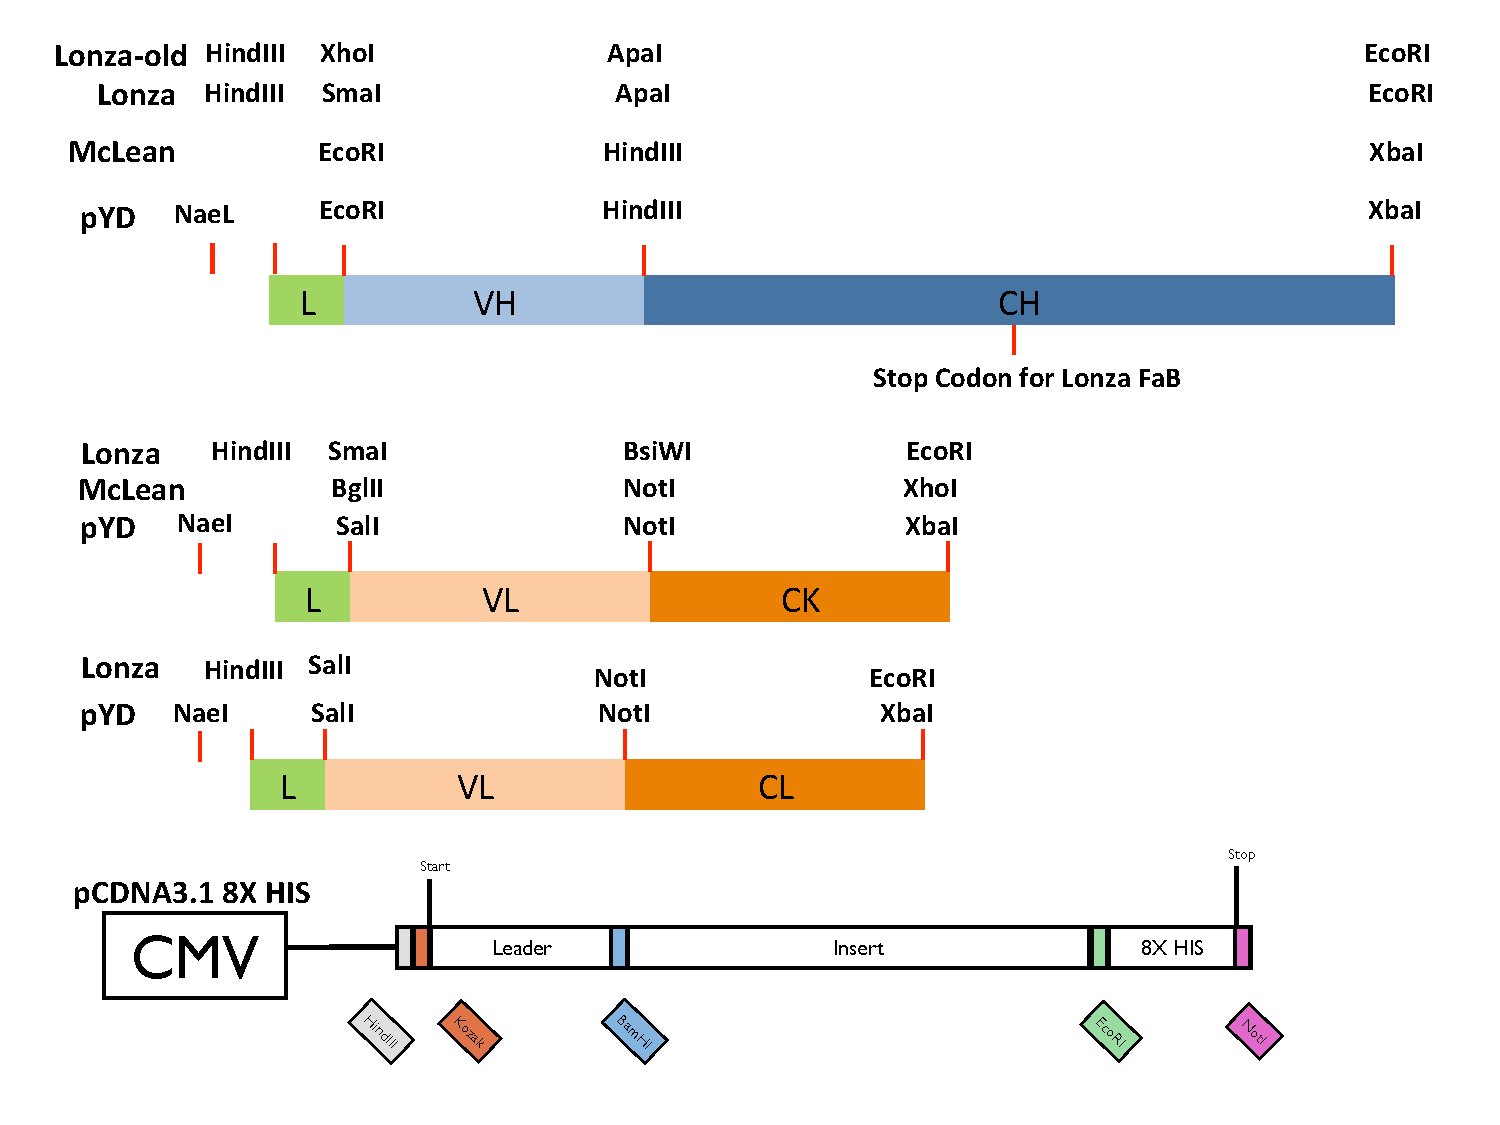
\includegraphics[scale=.85]{images/appendix/figa1.pdf}
   \caption[Restriction Maps for Common Vectors]{}
       \label{fig:figa_1}
\end{sidewaysfigure}

\clearpage

\subsection{HIV Neutralization Assay}
\textbf{Pre-Neutralization Assay} -
-Make growth media (GM) also called TZMbl media. (DMEM high glucose 1X + 110 mg/mL NaPy + 1X Pen-Strep +  10\% heat inactivated FBS)
-If you are testing serum, make sure to heat inactivate. \\

\textbf{Neutralization Assay}
Using the plate setup found in figure \ref{fig:figa_2}.
\begin{figure}[!t]
   \centering
   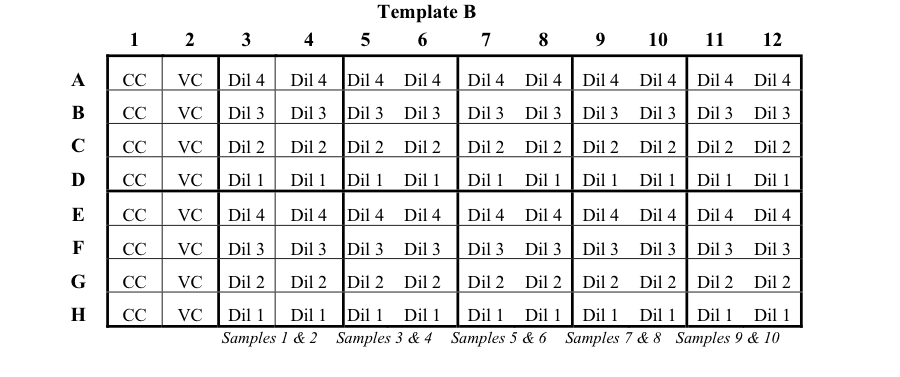
\includegraphics[]{images/appendix/figa2.png}
   \caption[Neutralization Assay Plate Setup]{}
       \label{fig:figa_2}
\end{figure}

\begin{enumerate}
  \item Put 150 \microliter~of GM into column 1
  \item Put 100 \microliter~of GM in the rest of the wells
  \item Start with 7.5 $\mu$g/mL of antibody in the Dil 1 wells (Row H, columns 3-12). This well be serially diluted 3 fold and give a final dilution of 0.2 $\mu$g/mL.
  \item Fill columns 3-12, row H up to 150 \microliter~with GM.
  \item Use 50 \microliter~of these rows to do a serial 3-fold dilution. Discard the 50 \microliter~out of the remaining row to ensure only 100 \microliter ~s left.
  \item Make a viral stock of 10 mL of GM to 4,000 TCID\textsubscript{50}. Viruses must be titered (see other protocols).
  \item Add 50 \microliter~of 4,000 TCID\textsubscript{50} stock to columns 2-12. Make sure you don't do column 1.
  \item Cover and incubate at $37\,^{\circ}\mathrm{C}$ for 2 hours.
\end{enumerate}

While the virus and antibodies are incubating. Prepare the cells to be added at the end of the incubation.

\begin{enumerate}
  \item TZMbl cells should be confluent. Decant cell culture and wash with sterile PBS.
  \item Add 5 mL of tryspin (to T150 flask) and incubate for 1 minute.
  \item Aspirate trypsin and incubate cells at $37\,^{\circ}\mathrm{C}$ for five minutes.
  \item Add 10 mL of growth media and count cells.
  \item Dilute cells in 500 mL falcon tube to 100,000/mL with GM.
  \item If it has been two hours, take the virus and antibody plates and add 100 \microliter of cells to every well.
  \item Cover and incubate at $37\,^{\circ}\mathrm{C}$ for 48-72 hours.
  \item From every well aspirate 100 \microliter~of GM.
  \item Add 100 \microliter~of Bright Glow Luciferase reagent and mix 10 times in every row. Incubate for 2 minutes.
  \item Record the luminescence on a luminometer.
  \item If background is low enough, \ic can be recorded from automatic PRISM non-linear regression analysis after log\textsubscript{2} transformation of concentrations.
\end{enumerate}



\clearpage
\section{Appendix V - Computational Standard Operating Procedures}
\label{sec:appenixV}
Here I will detail the computational procedures including running \rosetta~and analyzing data with scripts that are often available in the Meiler Lab Scripts repository or available on request. Also a lot of the procedures are detailed in IPython Notebooks and will also be available on request.

\subsection{Chapter I - Multi-State Design}
Here I will detail how I ran \rosettadesign~for multi-state design and how I analyzed the results. I will use the simplified example of IGH\textsubscript{V}5-51 which only contains three sets of molecular structures. There is a great protocol capture for complex procedures attached to the publication by Andrew Leaver-Fay showing how to \textit{design for} and \textit{design against} in multiple states \citep{LeaverFay:2011ji}.
\subsubsection{Running \rosetta~Multi-State Design}
To run multi-state design, I have to prepare several files.

\begin{itemize}
\item Entity File - A file containing the amount of residue positions to design as well as instructions for the packer to behave on all proteins. For example, we could want the packer only to use certain rotamers around the interface. This could be handled with the entity file.
\item Correlation File - Tells how residues correlate to each other. For example, residue 1 on protein A should be designed with residue 2 on protein B etc.
\item Secondary Residue File - This is a residue file as defined in the documentation, but will only instruct the packer to operate on each protein individually. Every state must have it's own secondary residue file.
\item Fitness File - A master file containing all other files as well as instructions for the fitness function.
\end{itemize}

\textbf{Clean PDB} - First, I can download all three protein PDBs with the clean\_pdb.py script. Clean PDB supports the following syntax:


\begin{lstlisting}[breaklines=true]
clean_pdb.py <PDB_ID> <CHAINS>
\end{lstlisting}

We only want the asymmetric unit in the crystal structure, so it helps to manually inspect the PDBs. We need one heavy chain, one light chain, and one antigen. I just go to www.pdb.org to find these chain codes.
\begin{lstlisting}
clean_pdb.py 2B1A HLP
clean_pdb.py 2XWT ABC
clean_pdb.py 3HMX HLB
\end{lstlisting}
Although not absolutely necessary, it makes it easier to label the chain IDs the same. All heavy chains have H, light L, and antigen A. There is a change PDB id script which allows us to quickly rename chain IDs. The script takes the following syntax.

\begin{lstlisting}[breaklines=true]
set_pdb_chain_id.py old_chain new_chain input output
\end{lstlisting}
I have looked through all the PDBs and figured out which names to change.

\begin{lstlisting}
set_pdb_chain_id.py P A 2B1A_HLP.pdb 2B1A_HLA.pdb
set_pdb_chain_id.py A H 2XWT_ABC.pdb 2XWT_HBC.pdb
set_pdb_chain_id.py B L 2XWT_HBC.pdb 2XWT_HLC.pdb
set_pdb_chain_id.py C A 2XWT_HLC.pdb 2XWT_HLA.pdb
set_pdb_chain_id.py B A 3HMX_HLB.pdb 3HMX_HLA.pdb
\end{lstlisting}
To ensure the starting structures use the correct numbering scheme, we should renumber each chain starting with 1.

\begin{lstlisting}[breaklines=true]
renumber_pdb.py 2B1A_HLA.pdb 2B1A_clean.pdb
renumber_pdb.py 2XWT_HLA.pdb 2XWT_clean.pdb
renumber_pdb.py 3HMX_HLA.pdb 3HMX_clean.pdb
\end{lstlisting}
Now we can remove all temporary files. Only *\_clean.pdb files should remain in the working directory. The next thing to do would be to find all positions with at least one difference. This requires manual inspection of the alignment. For the V\textsubscript{H} gene, there are 29 amino acid positions that will differ from germline in at least one position. These positions will be considered. Given that data, we can construct the entity residue file.

\begin{lstlisting}
#The entity.resfile
#The number of positions to design
29
#Allow all amino acids
#except cystine and use rotamer libraries 1,2
#and aromatic 2.
ALLAAxc EX 1 EX 2 EX ARO 2
#beginning of residue file
start
\end{lstlisting}

The correlation file maps how each residue in each file should map to the others. There will be three correlation files, one for each state. Since each amino acid lines up, i.e. design position 5 in 2B1A with position 5 in 3HMX, all the correlation files will be the same. Here is an example of one correlation file.

\begin{lstlisting}[breaklines=true]
#all.corr
#The first column is the entity,
#the second is the residue number for that state,
#the last is the chain.
1 5 H
2 14 H
3 16 H
4 23 H
5 24 H
6 29 H
7 30 H
8 31 H
9 32 H
10 34 H
11 40 H
12 46 H
13 48 H
14 51 H
15 52 H
16 54 H
17 58 H
18 65 H
19 70 H
20 72 H
21 74 H
22 76 H
23 77 H
24 80 H
25 84 H
26 88 H
27 93 H
28 97 H
29 98 H
\end{lstlisting}
A secondary residue file is also needed in case any extra packing tasks are needed to be supplied to each state. For example, we could tell one PDB state to design around the interface in single state design mode while everything in the correlation file designs together. I do not require extra design tasks for this protocol so all secondary residue files will be the same. For example,

\begin{lstlisting}[breaklines=true]
#tells the packer to use all natural side
#chain configurations for everything
#that is not being designed.
NATRO
#the input side chain is allowed
use_input_sc
#start the residue file
start
\end{lstlisting}

We next to create a states file that has the PDB, correlation file and secondary resfile names in it. Name them 2B1A.states, 2XWT.states, and 3HMX.states. They should look like the following when opened.

\begin{lstlisting}
#2B1A.states
input_files/2B1A_clean.pdb input_files/all.corr input_files/all.2res

#2XWT.states
input_files/2XWT_clean.pdb input_files/all.corr input_files/all.2res

#3HMX.states
input_files/3HMX.pdb input_files/all.corr input_files/all.2res
\end{lstlisting}

Lastly, a fitness file needs to be constructed to tell multi-state how to design. I call this file fitness.daf and it points to the locations of the states files.

\begin{lstlisting}[breaklines=true]
#initialize the states and what the states file name is
STATE_VECTOR A 2b1a.states
STATE_VECTOR B 2xwt.states
STATE_VECTOR C 3hmx.states


#tell design to minimize energy for each state
SCALAR_EXPRESSION best_A = vmin( A )
SCALAR_EXPRESSION best_B = vmin( B )
SCALAR_EXPRESSION best_C = vmin( C )

#Fitness - design to minimize all energies simultaneously
FITNESS best_A + best_B + best_C
\end{lstlisting}

\textbf{Running Rosetta Multi-State Design} \\
The \rosetta executable is called mpi\_msd.mpi.<operatingsystem>. It must be compiled in MPI mode as each state is assigned to a processor. The command line takes the following options.

\begin{itemize}
\item entity\_resfile - The resfile that we created in the input portion
\item fitness\_file - The fitness file we created in the input portion
\item ms::pop\_size - How many sequences to keep in memory at once (100 is a good number)
\item ms::generation - How many sequence generations should MSD go through see \citep{LeaverFay:2011ji} to find see how the genetic algorithm selects sequences.
\item ms::numresults - How many results to output. Will output top N sequences.
\item ms:fraction\_by\_recombination - How often should a cross-over even take place between sequences in the population. Read \citep{LeaverFay:2011ji} for details on the genetic algorithm.
\item database - The location of the database.
\end{itemize}

I construct an options file with all those options (options.txt) that looks like this.

\begin{lstlisting}[breaklines=true]
-entity_resfile entity.resfile
-fitness_file fitness.daf
-ms
    -pop_size 100
    -generations 435
    -numresults 100
    -fraction_by_recombination .04
-database my/rosetta/database/location/
\end{lstlisting}

Finally we can run \rosetta~using the following command after starting MPD.

\begin{lstlisting}[breaklines=true]
mpd && mpiexec -n 4 /my/rosetta/location/mpi_msd.mpi.myoperatingsystem \
@input_files/options.txt
\end{lstlisting}
\textbf{Warning! \linebreak \rosetta~may complain about some of the comments (anything starting with \#) not being recognized, if so, just remove it from the file}

The output will be 300 files, 100 for each of the states. We only need to analyze 100 files considering that the designed entities will be the same for all three files. For example, position 5 will be the same for 2B1A, 2XWT, and 3HMX.

\subsubsection{Analysis of MSD Output}
I wrote a design analysis script called deep\_analysis which encompasses many design analysis tools. I will only go into the functionality that is necessary to use, but you can read the options file for more use.

\begin{lstlisting}[breaklines=true]
deep\_analysis --help
>>              Design Analysis
___________________________________________________________

This script is intented to encompass the entire functionality
of design analysis. Everything you could want to do with design
is called upon in this script. The most basic functionality is
to pass a list of pdbs or get a position matrix of occurences
count of just one line.

The functionality extends from there by giving bitscores,
changes in energy, giving position specific scoring matrices
of your design,giving a customizable sequence logo. This is a
combination of many scripts and classes.

optional arguments:
  -h, --help show this help message and exit

Necessary:
  PDB files have to be included
  *.pdb  The PDB files to be analyzed

Recommended Options:
  Will give you a more complete analysis based on a res file,
  and a native pdb to compare it to.

  --native_pdb N_PDB, -p N_PDB
        The native pdb file to compare against
  --corr corr.corr, -c corr.corr
        Get the results defined only in the corr file
  --res resfile.resfile, -r resfile.resfile
        Get the results defined only in the residue file

Output Options: Please read carefully:
  These arguments change file name, which file is printed,
  which is output to a dictionary,and give verbose printing

  --verbose, -v
        everything printed to a file will also be shown
        on the screen
  --prefix PREFIX, -P PREFIX
        The prefix for what all the output files will be
  --score_files O_FILES [O_FILES ...], -s
    What do you want output to a file?
    Can list as a space seperated (eg -s n d nd):
    a - full analysis dict
    d - give analysis of just designed residues
    n - just the native residues scores are shown
    nd - just the native residues of the residues designed
            Defaults to full analysis dictionary
  -b Should the output be in bit score?
        Defaults to occurences instead of bitscore
  -S If you specify a native file and a design file,
        it will give you an output of the stats of the design

Rosetta Energy Analysis:
  Options for outputing options about energy scores,
  the dictionaries analyzed depend on what you asked
  for using the -s output options flag

  --rosetta, -t  This option will output a .csv file of the
  model,chain,residue,residue number,and rosetta scores.

Bit Score Options:
  options for bitscore metric for each designed residue

  -n    do you want the bit scores to be
        normalized by the shannon entropy

Sequence Logos Options:
  These options handle the sequence logos that can be output
  from the design analysis script, and uses the api of weblogo
  to do so.

  --seq, -l
    Turn on Sequence Logos for all the dictionaries
    you supply given in an .eps file
  --path LOGO\_PATH, -lp LOGO\_PATH
    What is the path to weblogo software?
    Defaults to meilerlab enviroment
  --format {eps,jpg,png,png_print,pdf,jpeg,svg,logodata}
    What format do you want the sequence logo in?
  --units {bits,nats,kt,kJ/mol,kcal/mol,probability}
    What do you want the units of the sequence
    logo to be in? Defaults to bits.
  --stacks S_STACKS
    How many sequences per line in the logo, default=after
    forty letters it will go to a new line.
  --stack_width S_STACK_WIDTH
    How wide is each stack in the logo. Value of 25 is useful
    for x-axis labels >3 characters and 30
    for labels as 'sequence_numbers'.
  --title S_TITLE
    The title of your sequence logo
  --x_label S_X_AXIS
    What do you want the x axis titled?
  --y_axis_height S_Y_HEIGHT
    How high do you want the Y axis,
    currently 4.32 which is the maximum
    acheivable score in a unbiased design
  --y_label S_Y_LABEL
    Title of Y-Axis
  --error_bars S_Y_ERROR
    Do you want error bars turned on, YES/NO?
  --fine_print S_FINE
    Fine Print
  --color_scheme
    {auto,chemistry,charge,classic,
    hydrophobicity,monochrome}
    The color scheme of the sequence logo.
    Defaults to Classic
  --labels {sequence,numbers,sequence_numbers}
    The x-axis labels can either take on the
    native residues sequence given with a native
    pdb file or the numbering of the pdb residue.
  --debug
    Get the full command line of what was put into weblo
\end{lstlisting}

It's obvious that this analysis can do a lot, but I will stick with the basics. First a new input that is completely germline. We can do this with the packer.
There is a script called make\_res.py which will make a residue file from a FASTA file. I use this to take the germline sequence and thread it over one of my inputs. Then that input can be used as our template.

\begin{verbatim}
>IGHV5-51*01
EVQLVQSGAEVKKPGESLKISCKGSGYSFTSYWIGWVRQMPGKGLEW
MGIIYPGDSDTRYSPSFQGQVTISADKSISTAYLQWSSLKASDTAMY
YCAR
\end{verbatim}

Then we can use the make\_res.py script.

\begin{lstlisting}[breaklines=true]
make_res.py IGHV5-51.fasta > IGHV5-51.res
\end{lstlisting}

This residue file can then be used to mutate one of our templates back to germline.
\begin{lstlisting}[breaklines=true]
/path/to/rosetta/bin/fixbb.default.<operating_system> \
-s 2B1A_clean.pdb \
-resfile IGHV5-51.res -database /path/to/database \
-out:path:pdb 2B1A_germline.pdb
\end{lstlisting}

Now we can use the analysis script.
\begin{lstlisting}[breaklines=true]
deep_analysis -p ../input/2B1A_clean.pdb \
-S -b -s nd -c ../input/all.corr msd_output_*A*.pdb

>>
#score vs mature
Total Bit Score of Design ===> 28.4534
Total Shannon Entropy of Design ===> 115.9577
Normalized Bit Score for design ===> 0.2454
\end{lstlisting}

and

\begin{lstlisting}[breaklines=true]
deep_analysis -p ../input/2B1A_germline.pdb \
-S -b -s nd -c ../input/all.corr msd_output_*A*.pdb

>>
#score vs mature
Total Bit Score of Design ===> 41.0967
Total Shannon Entropy of Design ===> 115.9577
Normalized Bit Score for design ===> 0.3544
\end{lstlisting}

This gives a design score towards 0.35 for the germline sequence and 0.24 for the mature sequence. Everything can be repeated this exact way. For single state design you can keep the fitness file exactly the same, but remove the other states.

\begin{lstlisting}[breaklines=true]
#initialize the states and what the states file name is
STATE_VECTOR A 2b1a.states
STATE_VECTOR B 2xwt.states
STATE_VECTOR C 3hmx.states


#tell design to minimize energy for each state
SCALAR_EXPRESSION best_A = vmin( A )
SCALAR_EXPRESSION best_B = vmin( B )
SCALAR_EXPRESSION best_C = vmin( C )

#Fitness - design to minimize all energies simultaneously
FITNESS best_A
\end{lstlisting}

And run the exact same procedures.

\subsection{Chapter II - Database and Design}
This section accompanies chapter \ref{chap:chapter2}. I will go over uploading the sequences to a database, selecting the correct sequences, threading, and finally design.

\subsubsection{Sequence Analysis}
The methods section detailed how I actually sequence the amplicons from 64 healthy donors, but processing them takes quite a bit of computational work. The VANTAGE core at Vanderbilt returns the sequencing runs as two paired end reads in FASTQ format. They must be ``stiched'' together to make one read. For example, for donor 10, there are ``2185-RC-10\_1.fastq'' for the forward read and ``2185-RC-10\_2.fastq'' for the reverse read. I use a stitching algorithm called ``pandaseq'' to process theses \citep{Bartram:2011cz}. These commands are incredibly simple to run.

\begin{lstlisting}[breaklines=true]
/usr/local/bin/pandaseq -f 2185-RC-10_1.fastq -r 2185-RC-10_2.fastq -T 23 > donor_10.fasta
\end{lstlisting}

Pandaseq will automatically output to the fasta format which is convenient for the next step. Here I use PyIg, my own sequence aligner against Ig mAbs that's based on IgBLAST \citep{Ye:2013bb}. I will probably publish this soon when it is more stable. For human IgG's it works incredibly simple to use.

\begin{lstlisting}[breaklines=true]
./PyIg
usage: igblast [-h] -q query.fasta [-d DB_PATH] [-i INTERNAL_DATA]
               [-a AUX_PATH] [-y {Ig,TCR,custom}] [-or {human,mouse}]
               [-nV NUM_V] [-nD NUM_D] [-nJ NUM_J] [-dgm D_GENE_MATCHES]
               [-s {imgt,kabat}] [-x EXECUTABLE] [-o OUT] [-t TMP]
               [-e E_VALUE] [-w WORD_SIZE] [-pm PENALTY_MISMATCH]
               [-nP NUM_PROCS] [-op OUTPUT_OPTIONS] [-z] [-c] [-j]

optional arguments:
  -h, --help            show this help message and exit

Necessary:
  These have to be included

  -q query.fasta, --query query.fasta
                        The fasta file to be input into igBlast

Database Paths:
  -d DB_PATH, --db_path DB_PATH
                        The database path to the germline repertoire
  -i INTERNAL_DATA, --internal_data INTERNAL_DATA
                        The database path to internal data repertoire
  -a AUX_PATH, --aux_path AUX_PATH
                        The auxilariay path that contains the frame origins of the germline genes for each repertoire.
                         Helps produce translation and other metrics

IgBlast Sprecific:
  IgBlast Specific Options with a Default

  -y {Ig,TCR,custom}, --type {Ig,TCR,custom}
                        Is this an IG or TCR recombination
  -or {human,mouse}, --organism {human,mouse}
                        The organism repeortire to blast against
  -nV NUM_V, --num_v NUM_V
                        How many V-genes to match?
  -nD NUM_D, --num_d NUM_D
                        How many D-genes to match?
  -nJ NUM_J, --num_j NUM_J
                        How many J-genes to match?
  -dgm D_GENE_MATCHES, --d_gene_matches D_GENE_MATCHES
                        How many nuclodtieds in the D-gene must match to call it a hit
  -s {imgt,kabat}, --domain {imgt,kabat}
                        Which classification system do you want

General Settings:
  -x EXECUTABLE, --executable EXECUTABLE
                        The location of the executable, default is /usr/bin/igblastn
  -o OUT, --out OUT     output file prefix
  -t TMP, --tmp TMP     temporary directory to store files in.
                        Defaults to ./tmp
  -e E_VALUE, --e_value E_VALUE
                        Real value for excpectation value threshold in blast.
                        Put in scientific notation
  -w WORD_SIZE, --word_size WORD_SIZE
                        Word size for wordfinder algorithm
  -pm PENALTY_MISMATCH, --penalty_mismatch PENALTY_MISMATCH
                        Penalty for nucleotide mismatch
  -nP NUM_PROCS, --num_procs NUM_PROCS
                        How many do you want to split the job across, default is the number of processors

Outputting Options:
  -op OUTPUT_OPTIONS, --output_options OUTPUT_OPTIONS
                        Open this file and comment out options you don't want in your final file.
                        The first column is the name of the option.
                        The second column is used by the parser and should not be changed.
  -z, --zip             Zip up all output files
  -c, --concatenate     Turn off automatic concatenation and deletion of temporary files.
                        Files are split up at the beginning to run across multiple processors
  -j, --json            Use the JSON output option that will format the text driven igblast output to a json document.
                        Defaults to CSV
\end{lstlisting}


I'll keep it simple for the protocol capture, but want to show how robust PyIg can be. Assume you are in the PyIg directory under PyIg/src/

\begin{lstlisting}[breaklines=true]
python2.7 execution.py -q donor_10.fasta -d datafiles/database/ -i internal_data/ -a datafiles/optional_file/ -y Ig -or human -nV 1 -nD 1 -nJ 1 -s imgt -o donor_10 -nP 23 -z -j
\end{lstlisting}

Each option is listed in the help. Make sure you see which each one does. For instance -nP needs to be carefully considered since it is the number or processors it will be run on. The output to this command line is a \.json file that will be uploaded to a Mongo database. One entry (with default output settings) looks like this.

\begin{lstlisting}[breaklines=true]
{
    "_id" : "donor_10_1000",
    "raw_seq" : "TGGAGCTGAGCAGCCTGAGATCTGAGGACACGGCCGTATATTACTGTGCGAAAGAACTATATGATAGTAGTGGTTATTACTACTTCCTGCCTTCTTACTACTACTACGGTATGGACGTCTGGGGCCAAGGGACCACGGTCACCGTCTCCTCAGGTAAG",
    "d_region" : "TATGATAGTAGTGGTTATTACTAC",
    "cdr3_aa" : "AKELYDSSGYYYFLPSYYYYGMDV",
    "fw4_aa" : "WGQGTTVTVSSGK",
    "full_seq_aa" : "AKELYDSSGYYYFLPSYYYYGMDVWGQGTTVTVSSGK",
    "cdr3" : "GCGAAAGAACTATATGATAGTAGTGGTTATTACTACTTCCTGCCTTCTTACTACTACTACGGTATGGACGTCTG",
    "top_d" : "IGHD3-22*01",
    "v_d_junction" : "ACTA",
    "top_j" : "IGHJ6*02",
    "cdr3_aa_length" : 24,
    "fw4" : "TGGGGCCAAGGGACCACGGTCACCGTCTCCTCAGGTAAG",
    "d_j_junction" : "TTCCTGCCTTCT",
    "d_or_j_junction" : "",
    "top_v" : "IGHV1-69*06",
    "full_seq" : "GCGAAAGAACTATATGATAGTAGTGGTTATTACTACTTCCTGCCTTCTTACTACTACTACGGTATGGACGTCTGTGGGGCCAAGGGACCACGGTCACCGTCTCCTCAGGTAAG",
    "full_seq_aa" : "AKELYDSSGYYYFLPSYYYYGMDVWGQGTTVTVSSGK",
    "d_bit_score" : 48.3,
    "d_evalue" : "3e-10.0",
    "d_alignment_length" : 24,
    "d_query_seq" : "TATGATAGTAGTGGTTATTACTAC",
    "d_subject_seq" : "TATGATAGTAGTGGTTATTACTAC",
    "d_percent_identity" : 100,
    "d_percent_positives" : 100,
    "d_mismatches" : 0,
    "d_positives" : 24,
    "d_identical" : 24,
    "d_subject_length" : 31,
    "d_score" : 24,
}
\end{lstlisting}

To download and install mongo, consult the manual \\ (http://docs.mongodb.org/manual/installation/). This installation will also include all the tools that making uploading files very easy. The output of PyIg should be ``donor\_10.json.gz''. We can then upload this json file to mongodb using the ``mongoimport'' application. \\

\textbf{Note:} \\
I assume you have an instance of MongoDB running.

\begin{lstlisting}[breaklines=true]
gunzip donor_10.json.gz & mongoimport -d test_database -c protocol_capture --file donor_10.json
\end{lstlisting}

Here I have made a database called test\_database and a collection called protocol\_capture. First thing to do is remove redundancies within mongo. To do that, I can make a simple index on the ``Input Sequence'' key and drop duplicates.

\begin{lstlisting}[breaklines=true]
db.protocol_capture.ensureIndex({'Input Sequence':1},{unique:true, dropDups:true})
\end{lstlisting}

The next thing I want to do is remove non-productive sequences. PyIg outputs a productive field, using mongo, I can tell the database to drop any ``document'' that contains a stop codon in the HCDR3.

\begin{lstlisting}[breaklines=true]
db.protocol_capture.remove({"Productive CDR3":"False"})
\end{lstlisting}

For \rosetta, I want only the thirty length HCDR3s. I can use ``mongoexport'' for this query along with an `awk' statement to get out the 30 length fasta files.

\begin{lstlisting}[breaklines=true]
mongoexport -d test_database -c protocol_capture -q '{"CDR3 AA Length":30}' --csv -fields "Sequence ID","CDR3 AA" | awk -F "," '{gsub("\"","",$1);gsub("\"","", $2);print(">"$1"\n"$2)}' > 30_length.fasta
\end{lstlisting}

This fasta file will be used in the remainder of the protocol. I will not go over all the different types of analysis I can do with this database for the purpose of this protocol.

\subsubsection{PSSM Heuristics}

Using the fasta file ``30\_length.fasta'' generated in the previous section, a quick script written in python to get random 2,000 sequences is shown below.

\begin{lstlisting}[breaklines=true, language=python]
from Bio import SeqIO
import random
handle = open('30_length.fasta')
records = SeqIO.parse(handle, "fasta")
dictionary = {}
for seq in records:
   dictionary[seq.id] = str(seq.seq)
random_dict = random.sample(dictionary.items(),2000)

with open('2000\_sequences.fasta') as f:
    for seq in random_dict:
        f.write(``>{0}\n{1}\n''.format(seq[0],seq[1]))
\end{lstlisting}

Using \rosettadesign, I will generate 2,000 resfiles that tell the packer to mutate the HCDR3 into each of the entries in the fasta file. To do this, there is a script available from the Meiler lab called ``fasta\_to\_resfile.py'' which will generate the resfiles necessary.

\begin{lstlisting}[breaklines=true]
fasta_into_res.py random_2000.fasta 95 126 H 0
\end{lstlisting}

The rest of the protocol uses \scripts~to do the design. For \scripts, you need an xml file, options file, and command line. The xml file is a scripting file that tells \rosetta~specific set of instructions (here I will name it threading.xml). The first step is relatively simple only doing a design and a full-atom minimization (called relax).

\begin{lstlisting}[breaklines=true, language=xml]
<dock_design>
    <SCOREFXNS>
    </SCOREFXNS>
    <FILTERS>
    </FILTERS>
    <TASKOPERATIONS>
     <InitializeFromCommandline name=ifcl/>
     <ReadResfile name=rr filename=%%resfiles%% />
    </TASKOPERATIONS>
        <MOVERS>
         <PackRotamersMover name=pr scorefxn=score12 task_operations=ifcl,rr/>
         <FastRelax name=fr task_operations=ifcl/>
        </MOVERS>
        <APPLY_TO_POSE>
        </APPLY_TO_POSE>
        <PROTOCOLS>
         <Add mover_name=pr/>
         <Add mover_name=fr/>
        </PROTOCOLS>
</dock_design>
\end{lstlisting}

The only caveat here is that we specify the resfile as a variable so the protocol does not have to be hard-coded. The command line will specify each resfile to give to the job. First, an option file must be produced as a simple text file.


\begin{lstlisting}[breaklines=true]
-in
    -path
        -database /my/rosetta/database/path
-out
    -pdb_gz
-parser
    -protocol threading.xml
-s input_pg9_no_antigen.pdb
-nstruct 100
\end{lstlisting}

Lastly the command line which will include the resfile as an option (named run.csh).

\begin{lstlisting}[breaklines=true]
#!/bin/csh
set res = $1
set out = `basename $res .resfile`
mpiexec -n 101 my/rosetta/pathrosetta_scripts.mpistatic.linuxgccrelease @flags.txt -out:prefix $out -parser:script_vars resfiles=${res} > out.log
\end{lstlisting}

And to run the command I simply use an awk script to generate all the commands.

\begin{lstlisting}[breaklines=true]
ls *resfile | awk '{system( "run.csh "$1 ) }'
\end{lstlisting}

\textbf{Note: This should be run on a computer cluster as 100 processors are needed in the above protocol}

The next step is to run the output PDB files and generate a position-specific scoring matrix. This is easily accomplished with the ``create\_pssm\_from\_threading.py'' script that is also found in the Meiler lab scripts repository. A simple command to generate a PSSM.

\begin{lstlisting}[breaklines=true]
./create_pssm_from_threading.py -g -r resfiles/donor\_10\_991403.resfile -n 2000.p3sm *.pdbs
\end{lstlisting}

The output .p3sm can now be used to predict the top N sequences from the 30\_length.fasta generated earlier in the protocol.

\begin{lstlisting}[breaklines=true]
./create_pssm_from_threading.py -r resfiles/donor\_10\_2832895.resfile -s -p 2000.p3sm 30\_length.fasta
\end{lstlisting}

This generates a file called ``scored\_fasta.output''. I use awk and some other gnu commands to get the top 1000 scored fasta files.

\begin{lstlisting}[breaklines=true]
sort -nk 3 scored_fasta.output | head -n 1000 | awk '{print(">"$1"\n"$2)}' > top1000.fasta
\end{lstlisting}

Finally, I can make all the resfiles using the same command as before.

\begin{lstlisting}[breaklines=true]
fasta_into_res.py top1000.fasta 95 125 H 0
\end{lstlisting}

For the full design protocol using these sequences and resfiles. See the next section on PG9 redesign (subsection \ref{subsec:pg9redesign}).

\subsection{Chapter III - PG9 Design}
\label{subsec:pg9redesign}
\setlength{\parindent}{0cm}
This protocol capture will detail the how to use \rosettadesign~to predict mutations that enhance specificity. This accompanies the manuscript Willis \textit{et al.} \textbf{\textit{Nature Med.}} (submitted). It assumes that you have a \rosetta~license from www.rosettacommons.org. \\

\subsubsection{Preparing the input files}
Using PG9/CAP45 complex, I have prepared a \rosetta~compatible file called PG9\_input.pdb. This has spcecial identifiers for the glycans that \rosetta 's database can understand. To create your own glycan input, an excellent protocol capture is provided in an accompanying manuscript by Doug Renfrew \citep{Renfrew:2012ci}. \\

The design protocol used runs through the following steps.

\begin{itemize}
\item Favor native residue - gives bonuses to sequences which match PG9\textit{wt}
\item Design/minimize/dock iteratively
\item Constrain movements so glycans retain input position
\item Relax the energy of the structure
\item Re-dock
\item Score binding energy and structure energy
\end{itemize}

For this redesign we need several input files. The XML script, options file, residue file, and constraint file. The most complex of which, the XML file, informs Rosettaof our protocol. Use the following .xml file which is found under:

\begin{verbatim}
/input_files/threading_design.xml
\end{verbatim}

\textit{XML-File}
\lstinputlisting[breaklines=true]{input_files/threading_design.xml}


The behavior of the these instructions is described fully in \citep{Fleishman:2011ji}. They are divided up into a set of movers, filters and task of operations. All of the movers and filters along with their options are explained at the Rosetta Commons users guide (https://www.rosettacommons.org/docs/latest/RosettaScripts.html). \\

\textit{Options-File}\\
The options file are passed to the application. Defines output and input options as well as other options which can't be defined in the XML file.

\lstinputlisting[breaklines=true]{input_files/threading.txt}
Each option is explained with a \# comment.\\

\textit{Residue File}\\
The residue file tells the packer how to design the protein. The first line lets the packer use the side chains of the input PDB even if they are not in the rotamer libraries. The ``NATAA'' lines tells the packer to use input amino acid for everything not defined under start. In other words it will only design everything under start. The first column is the residue number, the second is the chain, and ``ALLAA'' tells the packer to use all amino acid identities at this position. For complete documentation of the resfile, visit https://www.rosettacommons.org/docs/latest/resfiles.html

\lstinputlisting[breaklines=true]{input_files/normal_design.resfile}

\textit{Constraint File} \\
The constraint file ensures that the glycan's are involved in binding. The torsional angles of the glycan can cause major structural perturbations.
\lstinputlisting[breaklines=true]{input_files/glycan_constraints.cst}

The constrain file syntax is found in the documentation - \\(https://www.rosettacommons.org/docs/latest/constraint-file.html). Briefly, I define two atoms with the input crystal structure distances. If these are violated, then there is an energetic penalty. \\

\subsubsection{Running \rosetta}
To run \rosetta, I use an application called \scripts~\citep{Fleishman:2011ji}. Since we have defined all the input files. Running the application only requires passing the options file.

\begin{lstlisting}[breaklines=true]
my/path/to/rosetta/source/bin/rosetta_scripts.myoperatingsystem @input_files/threading.txt -database my/path/to/rosetta/database/
\end{lstlisting}

This protocol generates 200 models each taking approximately 1 hour to complete. It is best to run this protocol on a computational cluster with each node producing a separate model (-nstruct 1). All files are output into a directory output models/. There are 200 pre-generated models for analysis. \\

\subsubsection{Analyzing Models}
There are three scripts in the /analysis folder that are used to analyze the mutations. Score\_vs\_rmsd full.py will give all the models energies as well as how much they deviated from the original structure. Get\_per\_ddg.py will give all of the binding energies decomposed by residues. Scores\_decomposed\_by\_resfile.py will decompose the energies of HCDR3 loop. They are each run using the following.

\begin{lstlisting}[breaklines=true]
score_vs_rmsd_full.py −m −n ../input_files/pg9_input.pdb −o s_v_rmsd −r ../input_files/normal_design.resfile ../output_files/∗.pdb

get_per_ddg.py -m -o per_ddg ../output_files/∗.pdb

scores_decompose_by_resfile.py −m −o HCDR3 −r ../input_files/normal_design.res
\end{lstlisting}

These will yield a series of data files that can be uploaded to a database or in a spreadsheet viewer. The complex queries I used to check energies between \text{wt} and mutations are beyond the scope of a protocol capture. But you can contact jwillis0720@gmail.com if you need additional guidance.







\singlespacing
\renewcommand\bibname{References}
\bibliographystyle{apalike}
\bibliography{full_library}
\end{document}
